\newpage
\section{评估NVIDIA新架构GPU的机器学习应用性能}
\setcounter{table}{0}
\setcounter{figure}{0}
\subsection{实验工具与环境}
\par 表 \ref{table-环境}和表 \ref{table-实验工具}中列出了实验环境与若干软件工具。\\
\begin{table}
	\centering
	\renewcommand{\thetable}{\arabic{section}-\arabic{table} }
	\renewcommand{\tablename}{表}
	\caption{实验环境}
	\addtocounter{table}{-1}
	\renewcommand{\thetable}{\arabic{section}-\arabic{table} }
	\renewcommand{\tablename}{Table}
	\caption{Environment}
	\begin{tabular}{cc}
		\toprule
		项目	&	内容\\
		\midrule
		CPU		&	AMD Ryzen ThreadRipper 2990WX 32C64T @ 3.0GHz\\
		主板		&	MSI X399\\
		内存		&	CORSAIR DDR4 3200 @ 16-15-15-15-34-1T 128GB\\
		GPU		&	NVIDIA Geforce RTX 2080TI (Turing)\\
		硬盘		&	INTEL750 NVMe PCIe 1.2TB * 2 @ RAID 0\\
		系统		&	Windows 10 64-bit build 17763\\	
		CUDA	&	Ver. 10.1, 10.0, 9.2, 9.0\\
		CUTLASS & Ver. 1.2, 1.3\\
		其他		&	Jetson TX2 $ * $\\
		\bottomrule
	\end{tabular} 
	\label{table-环境}
	
	$ * $该硬件由NVIDIA提供。\\
\end{table}
\begin{table}
	\centering
	\renewcommand{\thetable}{\arabic{section}-\arabic{table} }
	\renewcommand{\tablename}{表}
	\caption{实验工具}
	\addtocounter{table}{-1}
	\renewcommand{\thetable}{\arabic{section}-\arabic{table} }
	\renewcommand{\tablename}{Table}
	\caption{Tools}
	\begin{tabular}{cc}
		\toprule
		项目	&	内容\\
		\midrule
		Python 3.6		&	用于进行数据统计、编写TensorFlow应用\\
		Conda 4.5.12		&	用于创建、管理、隔离Python环境\\
		TensorFlow		&	1.12.0和1.13.0版本的源码,用于对比、研究、调整\\
		Bazel 0.16.0		&	用于从源码构建TensorFlow\\
		Msys2		&	用于从源码构建TensorFlow\\
		CMake 3.1.0		&	用于构建CUTLASS\\	
		Nsight 6.0	&	用于后台监听CUDA应用,捕捉Trace\\
		nvprof		&	用于分析CUDA程序的API调用、分支效率等\\
		git			&	版本控制\\
		Perforce	&	版本控制\\
		Ubuntu 16.04 Physical & 用于执行GPGPU-SIM 应用\\
		GPGPU-SIM 3.2 & 用于从指令级别模拟CUDA程序\\
		Visual Studio 2017 & 搭配10.0.17763.0版本的SDK\\
		\bottomrule
	\end{tabular} \label{table-实验工具} 
\end{table}
\subsection{基于测试样例的Benchmark}
\par 为了为接下来的实验设定基准,这一步先使用用途单一的测试样例测试绝对性能以及相应的提升,因不同架构的硬件各项参数(包括流处理器数量、显存容量等)不尽相同,所以直接对比不同架构硬件的性能是没有意义的,这里选择对比不同架构硬件在不同SDK下性能提升的比例。此处选用了CUDA 10.0,CUDA 9.2,CUDA 9.0三种SDK,同时选用9.2与9.0的原因是因为9.2版本是为了图灵架构的GPU Tesla V100发布的\cite{CUDA92},也在本文的研究范围内。
\par 因为本文主要讨论新架构GPU在机器学习应用中带来的性能提升,故选用的评测样例大部分都与机器学习应用相关;主要从以下角度进行评估:通用矩阵乘法(GEMM, General Matrix Multiply)、矩阵乘法运算性能、卷积运算性能、神经网络推理性能以及结合框架的综合性能。在评估这些性能时也会包含单/双精度浮点计算性能。
\subsubsection{通用矩阵乘法运算(GEMM, General Matrix Multiply)}
\par 作为新硬件最为鲜明的特点,本节将对张量核心以及相应的通用矩阵乘法运算进行评估,通用矩阵乘法运算又被称为混合矩阵运算,其混合体现在:运算中同时有加法和乘法,且精度同时涉及半精度浮点、单精度浮点和8位整数。与矩阵乘法相比,通用矩阵乘法被定义为:
$$ C \leftarrow \alpha AB + \beta C $$
\par 若将$ \beta $置为0,则该运算变为矩阵乘法运算。通用矩阵乘法这一运算在神经网络训练、推理中十分常见,根据官方文档,目前张量核心仅能用在CNN/RNN等特定结构的神经网络上,且只能用于前馈和反馈两部分。这个范围看起来很宅,然而在深度学习中占到了非常高的比重。式中操作数分别代表输入、权重和偏置,下文将简写为矩阵乘加。NVIDIA在新的伏特架构与图灵架构中加入的张量核心(Tensor Core)正是专门加速这种运算的硬件。
\paragraph{实验结果}
\par 根据开发者社区的反映,新架构硬件性能的差别主要体现在问题规模、问题类型等方面(张量维度、形状,训练/推理任务等),而NVIDIA官方仅给出一种规模的结果,所以本节使用了自行编写的一系列测试用例,辅以深度学习测试套件DeepBench\cite{DEEPBENCH},在开启和关闭新架构中张量核心的情况下进行测试。实验性能使用TFlops/s统计,方法为简单的运算数除以运算时间,运算时间的统计采用CUDA内置的$ cudaEvent $记录。
\par 首先评估的是在不同问题规模下,开启和关闭新架构中的张量核心所能达到的性能,如图 \ref{Fig-PerfGemm}所示。随着问题规模的上升,总体加速比呈上升趋势,在大规模数据时半精度通用矩阵运算性能的加速比能达到3到3.5倍、单精度通用矩阵运算性能的加速比能达到2倍。然而,单纯考察数据规模发现加速比差距非常大,甚至是在大规模数据中仍然存在开启张量核心后性能不如不开启张量核心的情况,结合文档在通用矩阵运算一章中在指令中需要指明运算的最小单元这一点中\cite{PTX};可以推测出输入矩阵的“形状”对张量核心的性能由较大影响。
\par 为了研究输入矩阵“形状”对于加速比的影响,由于两个输入矩阵涉及三个维度,故采用控制变量法,控制$ m,n,k $中某一维度考察另外两个维度对于加速比的影响。由于测试数据中存在部分离群值($ N\geq 500000 $),这会对作图精度产生极大影响,故先予以剔除。实验结果如图 \ref{Fig-MNKRatio}所示。可见在两个输入矩阵的三个维度中,两矩阵共享的维度$ K $对于性能的影响最为显著。
\par 关于矩阵的形状、维度对于性能的影响,其原因将在后文结果分析中详细说明。以上实验数据以及性能旨在考查开启和关闭张量核心时性能提升幅度,故开启的线程块数量和线程数量较小,相应的GPU占用率也较小,导致所得性能并非GPU峰值性能。为测量峰值性能,这里还是用NVIDIA官方发布的用于线性代数计算的模板库CUTLASS(CUDA Template Linear Algebra Subroutines),该模板库根据新架构硬件特性编写,提供了许多测试样例供参考,目前版本已经更新到1.3,相比于1.2使用了新加入CUDA SDK 10.1的mma.sync以优化性能,这里使用CUTLASS测试得到的性能作为峰值性能基准。
\par CUTLASS库中的GEMM运算有多种精度可供选择:HGEMM、SGEMM、DGEMM、CGEMM、ZGEMM和IGEMM,分别代表半精度浮点、单精度浮点、双精度浮点、单精度复数、双精度复数和八位整数。鉴于之前的测试并不涉及复数,此处也不选用复数精度作为基准。需要注意的是测试样例后缀中存在$ \_[n/t][n/t] $分别代表运算中输入矩阵的数据存储、分布方式,即行列是否转置(如上文提到的,CUDA中矩阵存储分行主元素和列主元素存储)。图 \ref{Fig-GEMM-CUTLASS}为测得的性能基准。
\begin{figure}
	\centering
	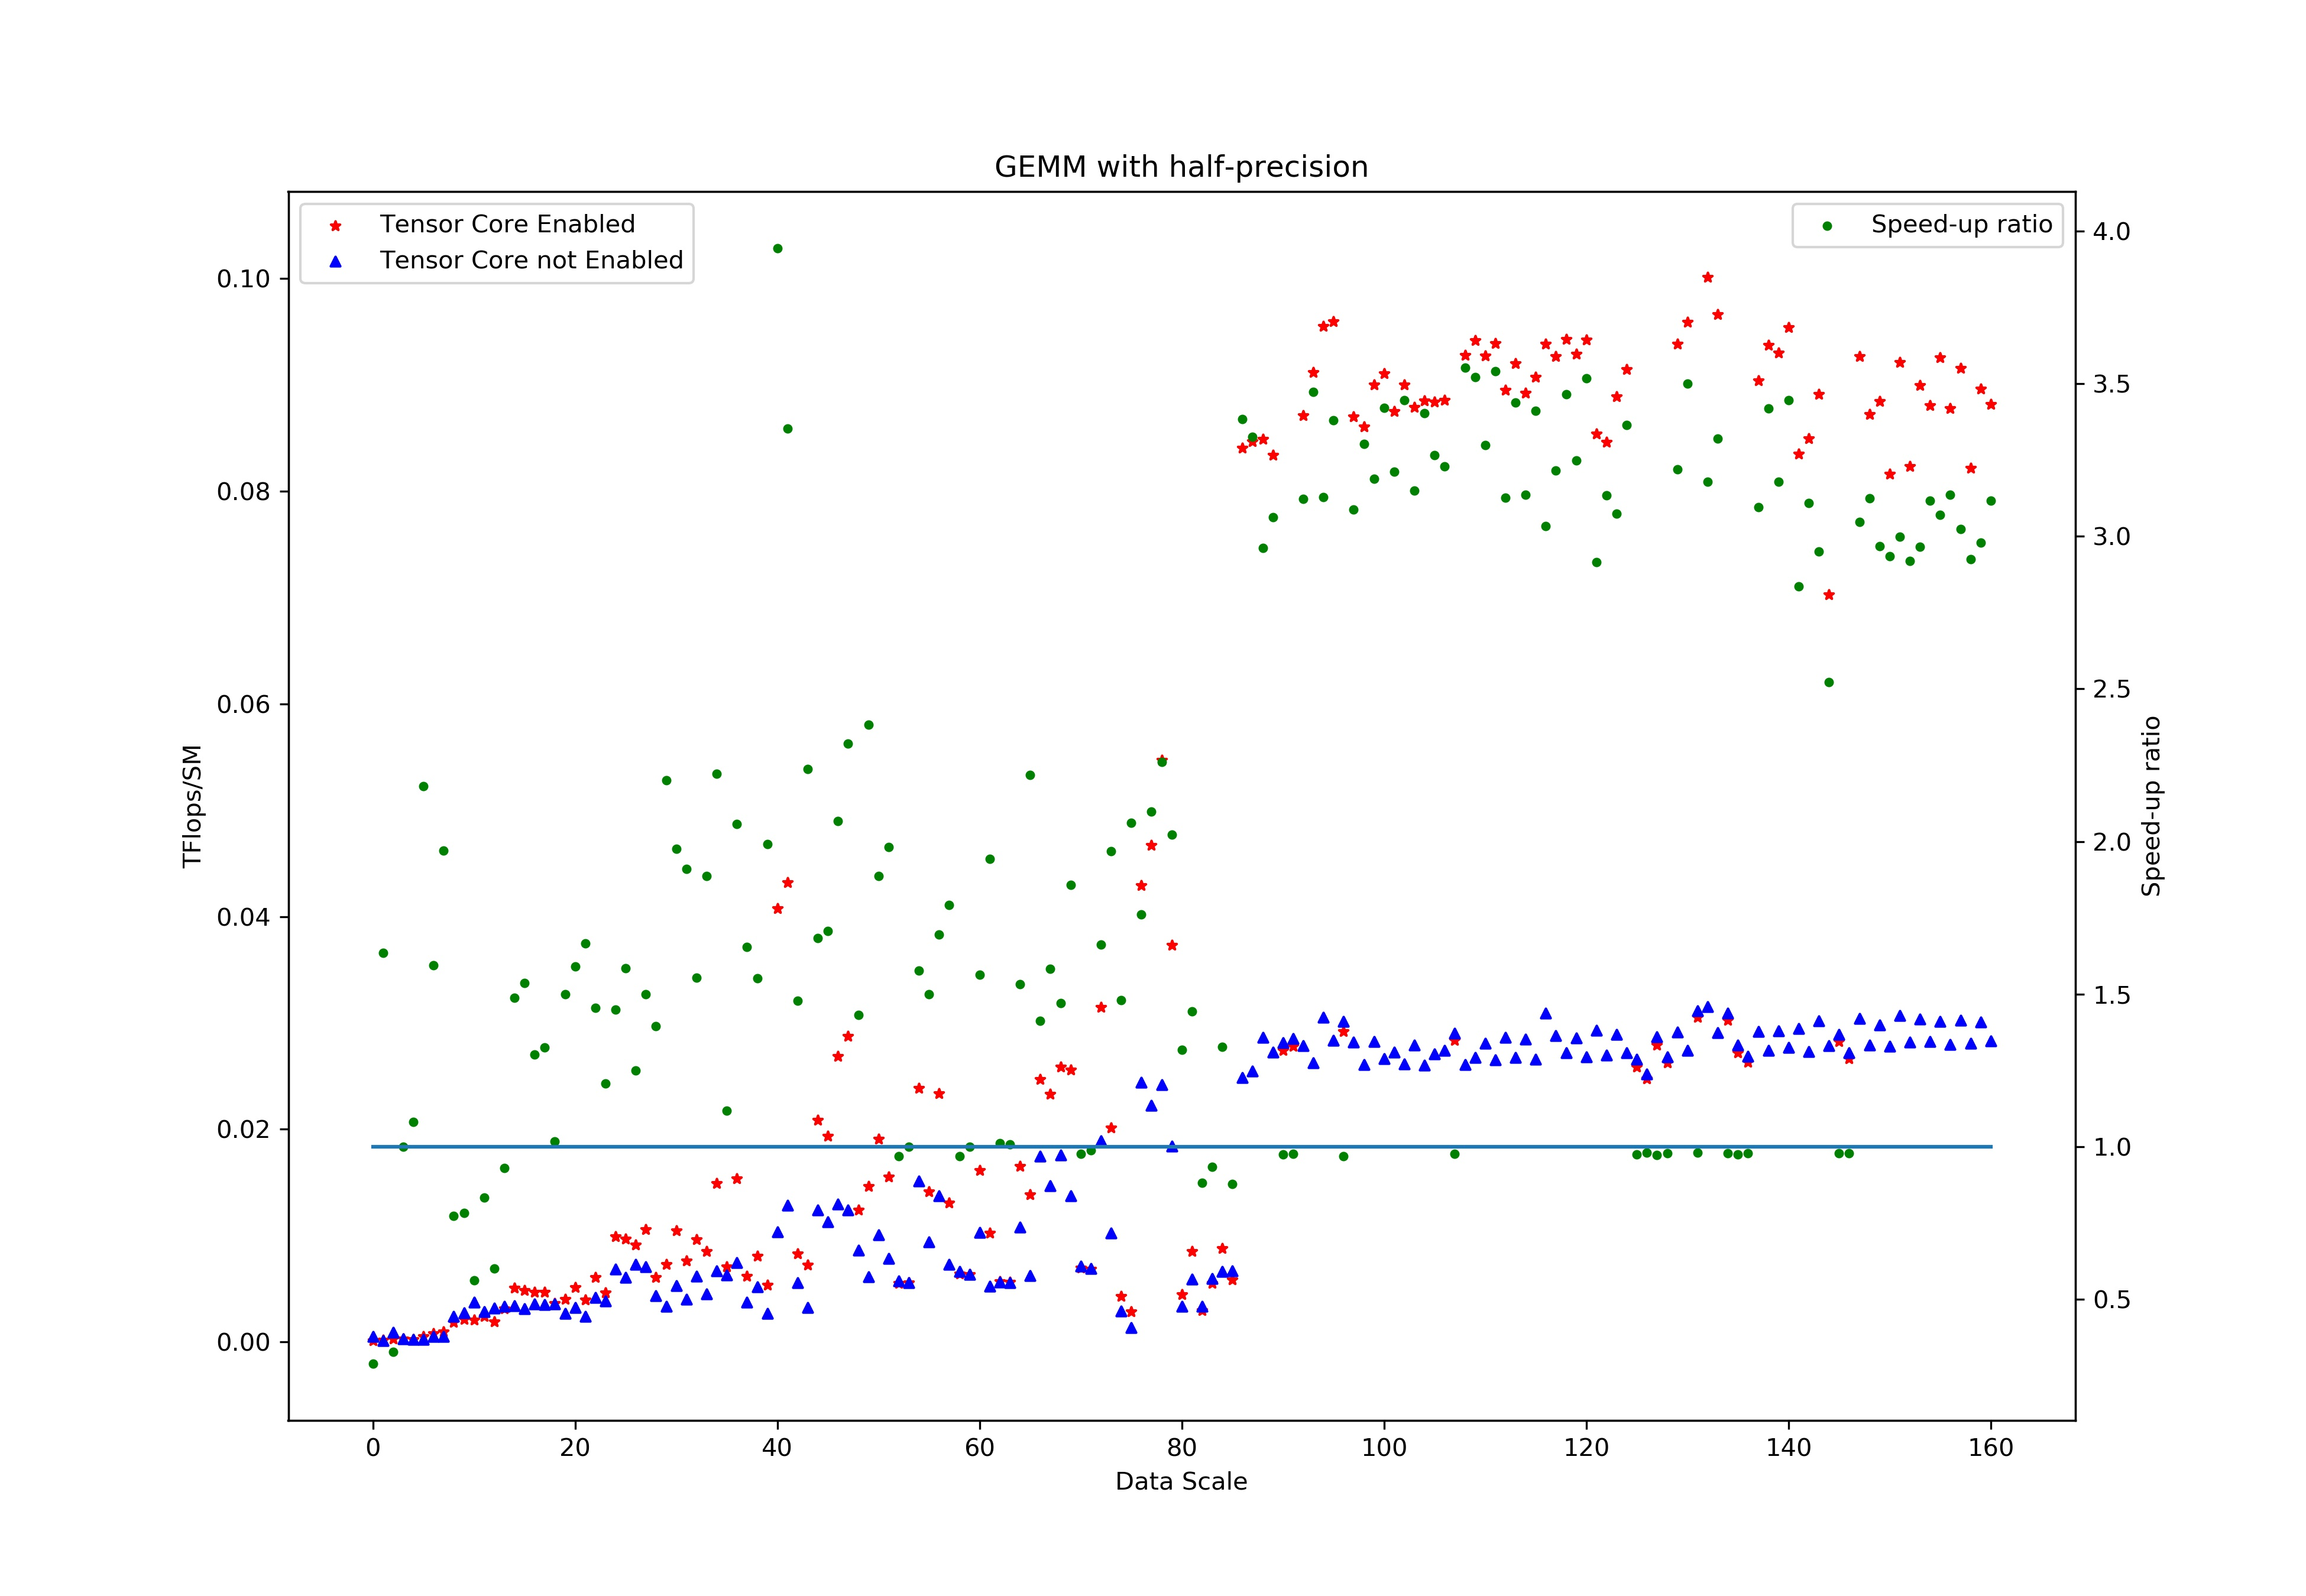
\includegraphics[width=15cm]{figures/GEMM-Half-TF.jpg}\\
	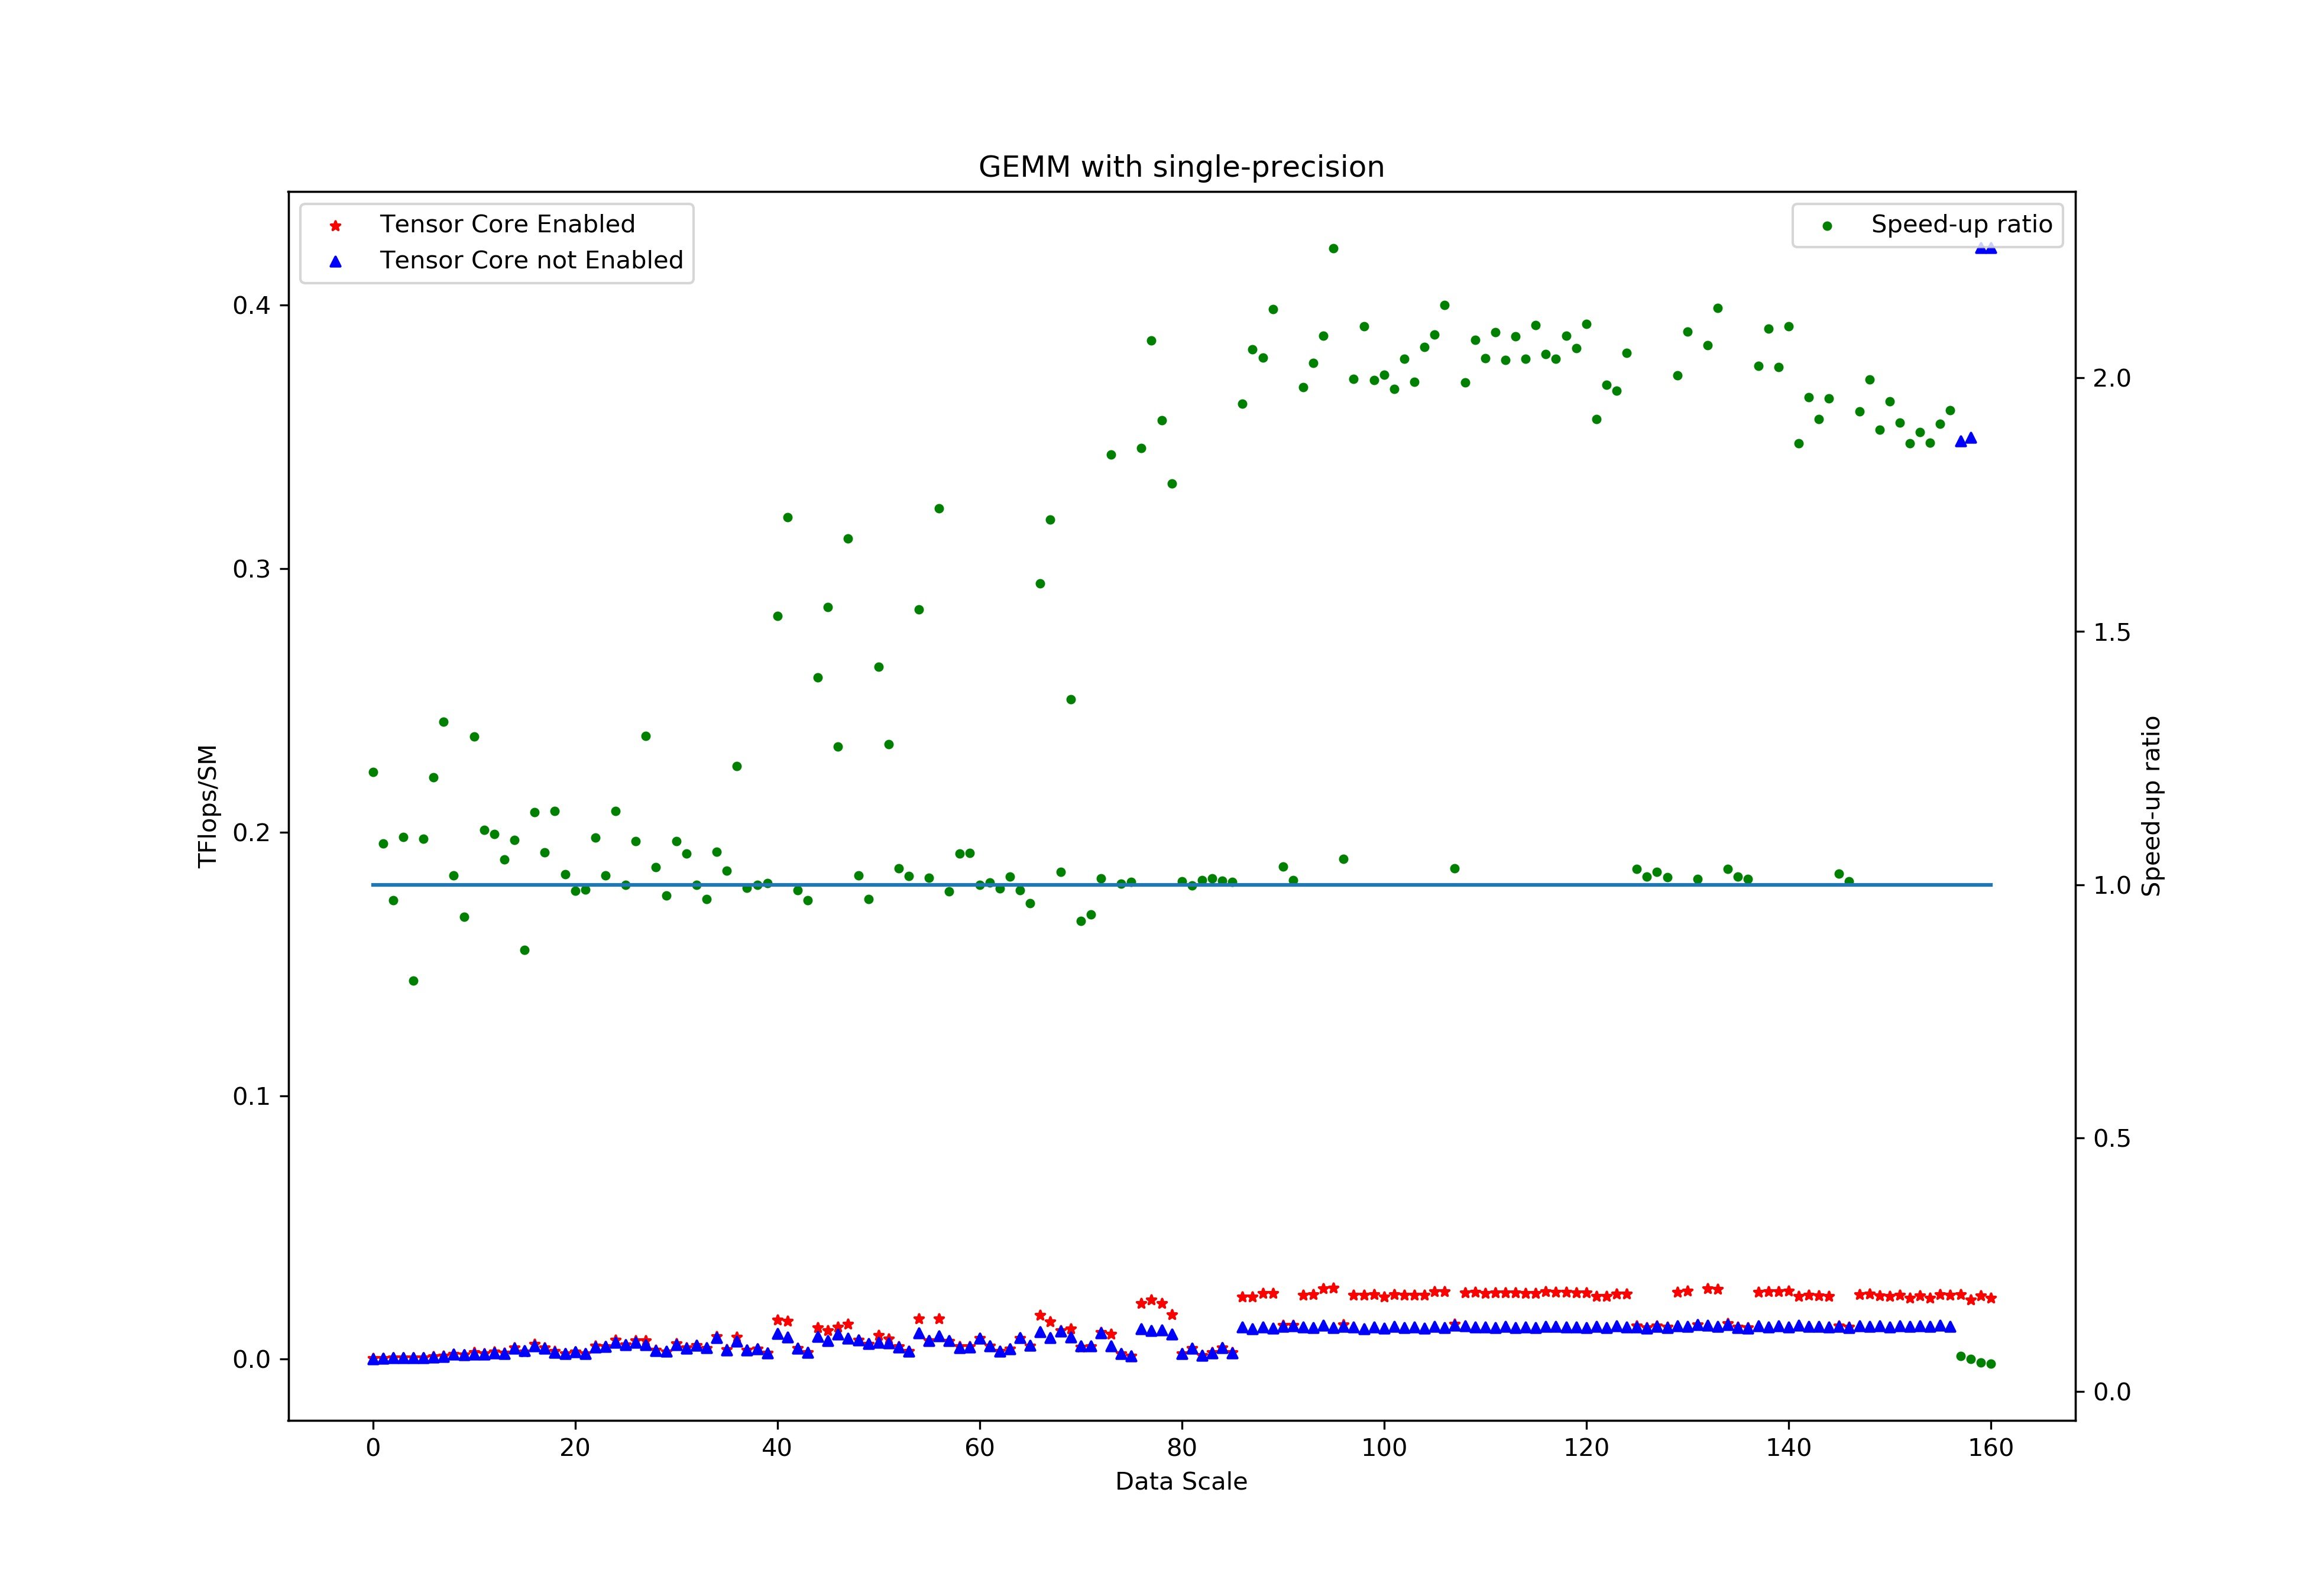
\includegraphics[width=15cm]{figures/GEMM-Single-TF.jpg}
	\renewcommand{\thefigure}{\arabic{section}-\arabic{figure} }
	\renewcommand{\figurename}{图}
	\caption{半精度/单精度GEMM性能}
	\addtocounter{figure}{-1}
	\renewcommand{\thefigure}{\arabic{section}-\arabic{figure} }
	\renewcommand{\figurename}{Figure}
	\caption{Performance of GEMM at Half and Single}
	\label{Fig-PerfGemm}
\end{figure}
\begin{figure}
	\centering
	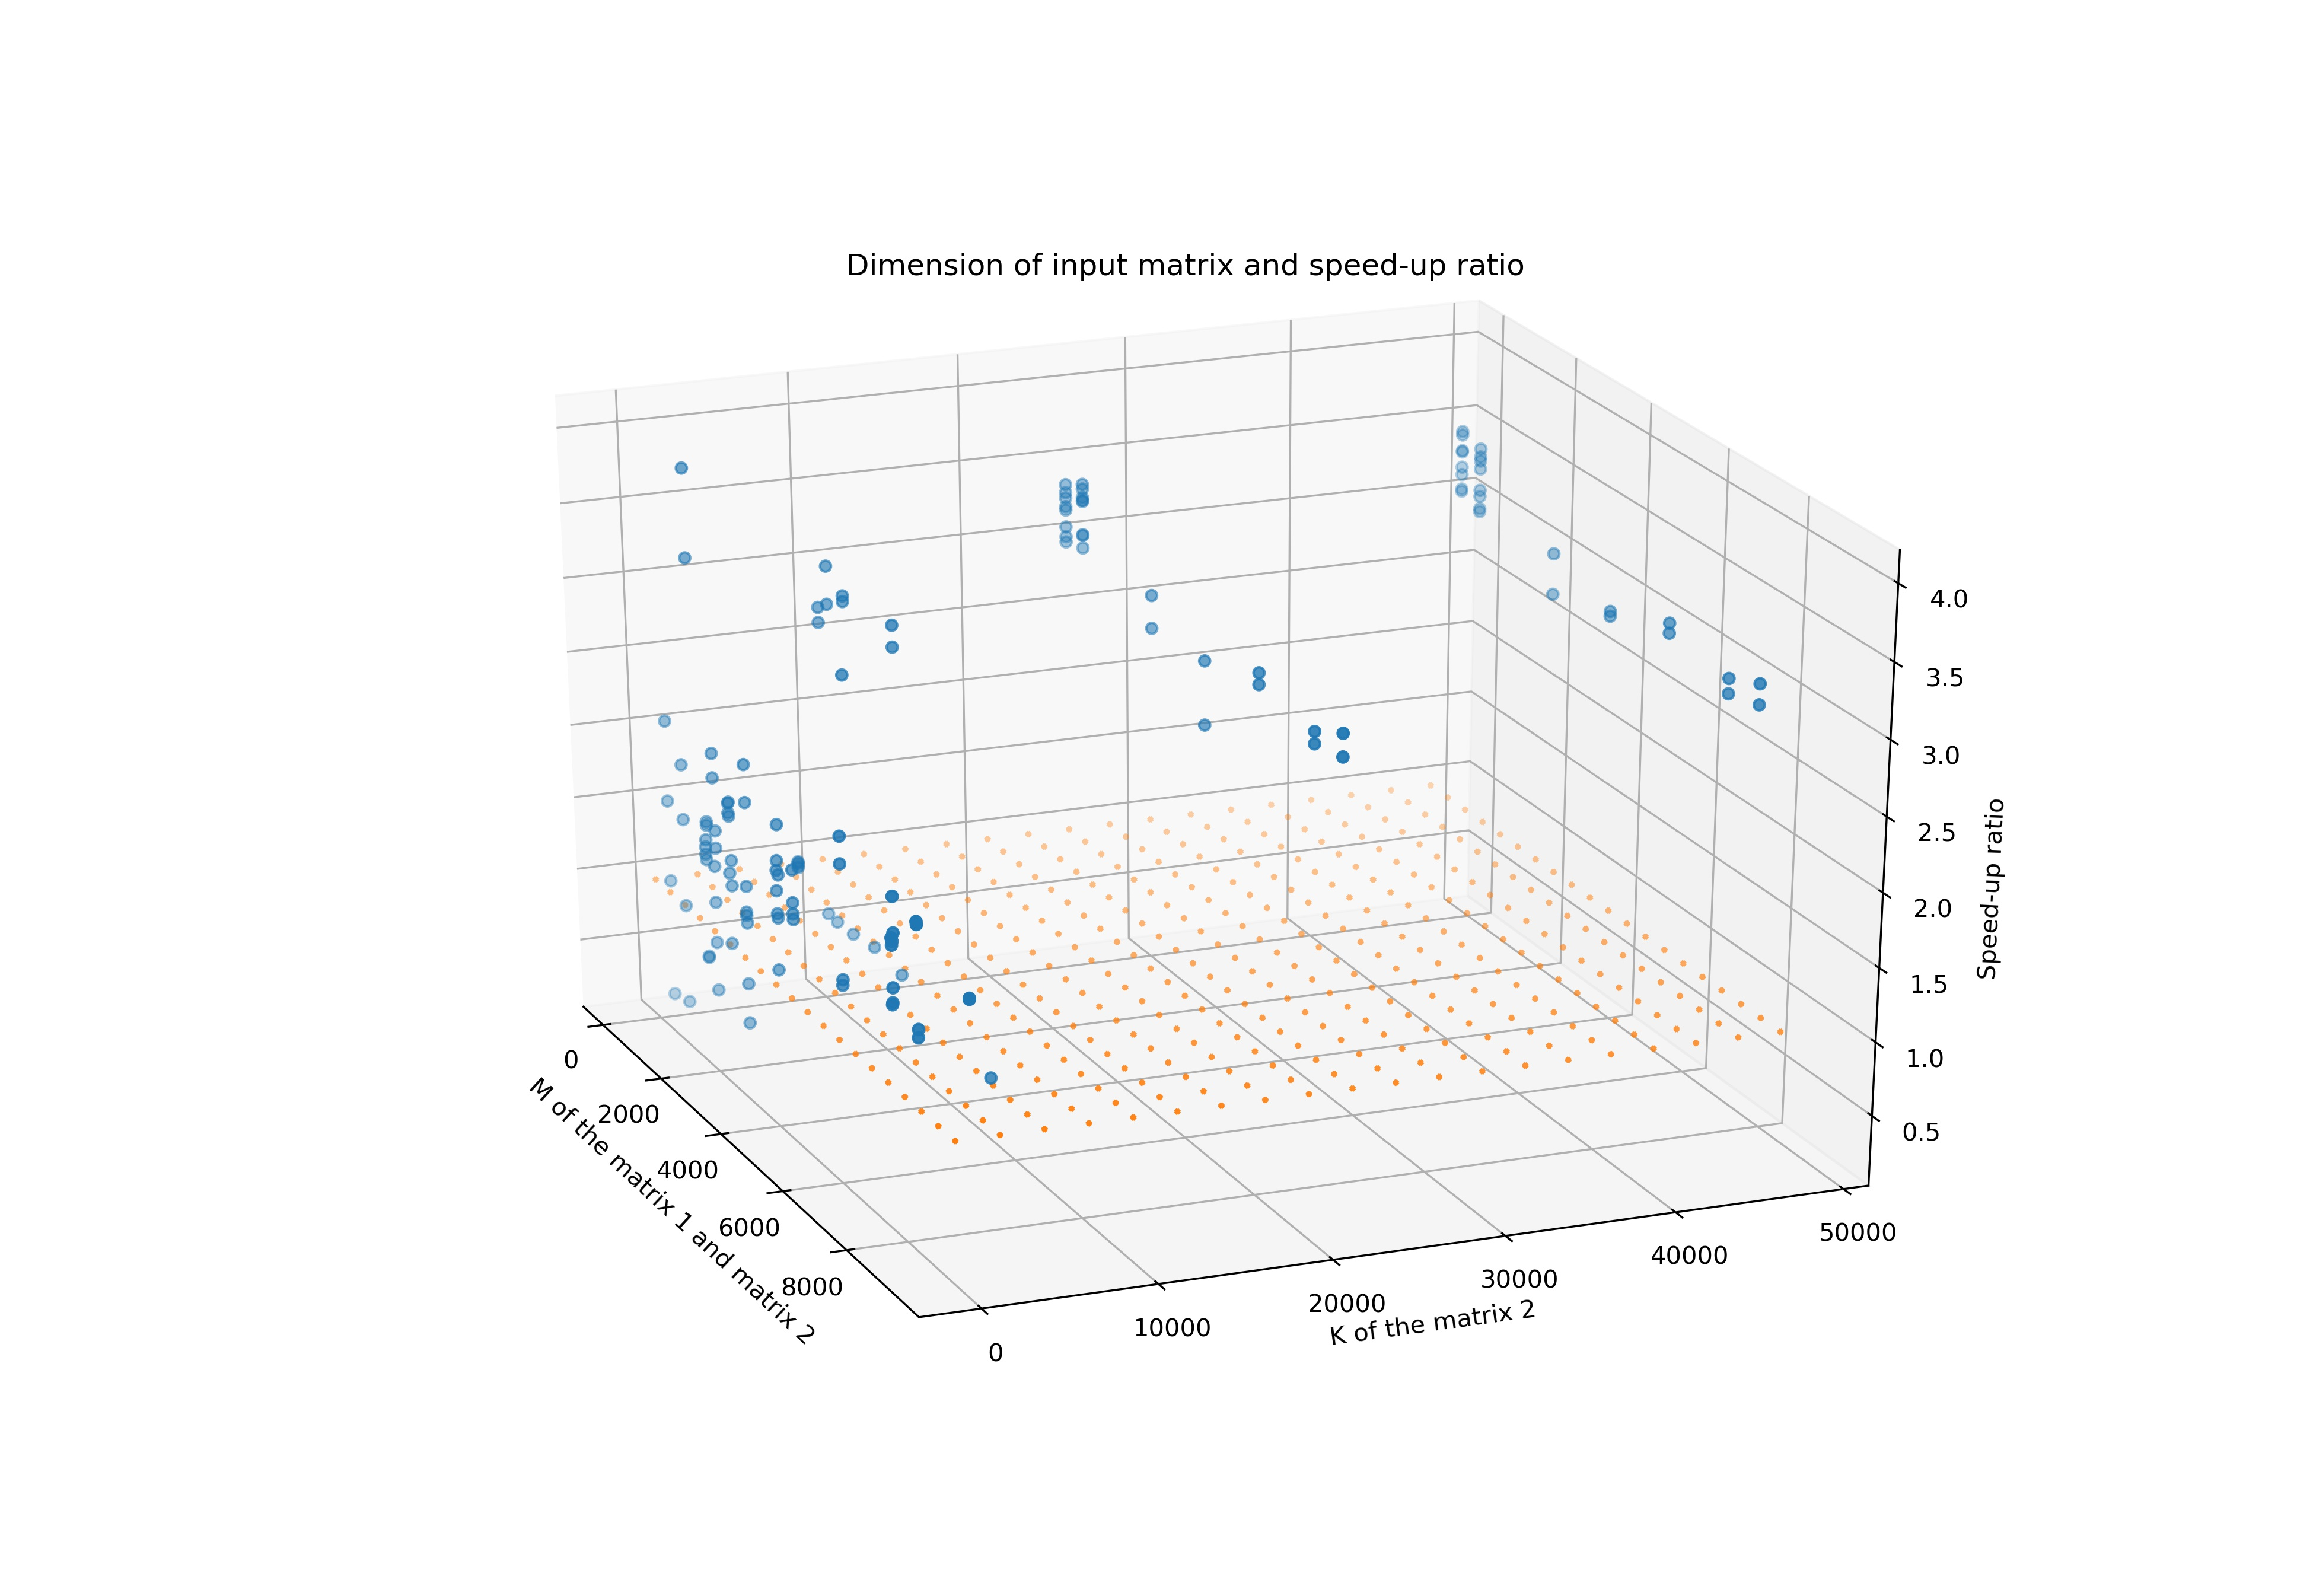
\includegraphics[height=7.2cm]{figures/GEMM_MK.jpg}\\
	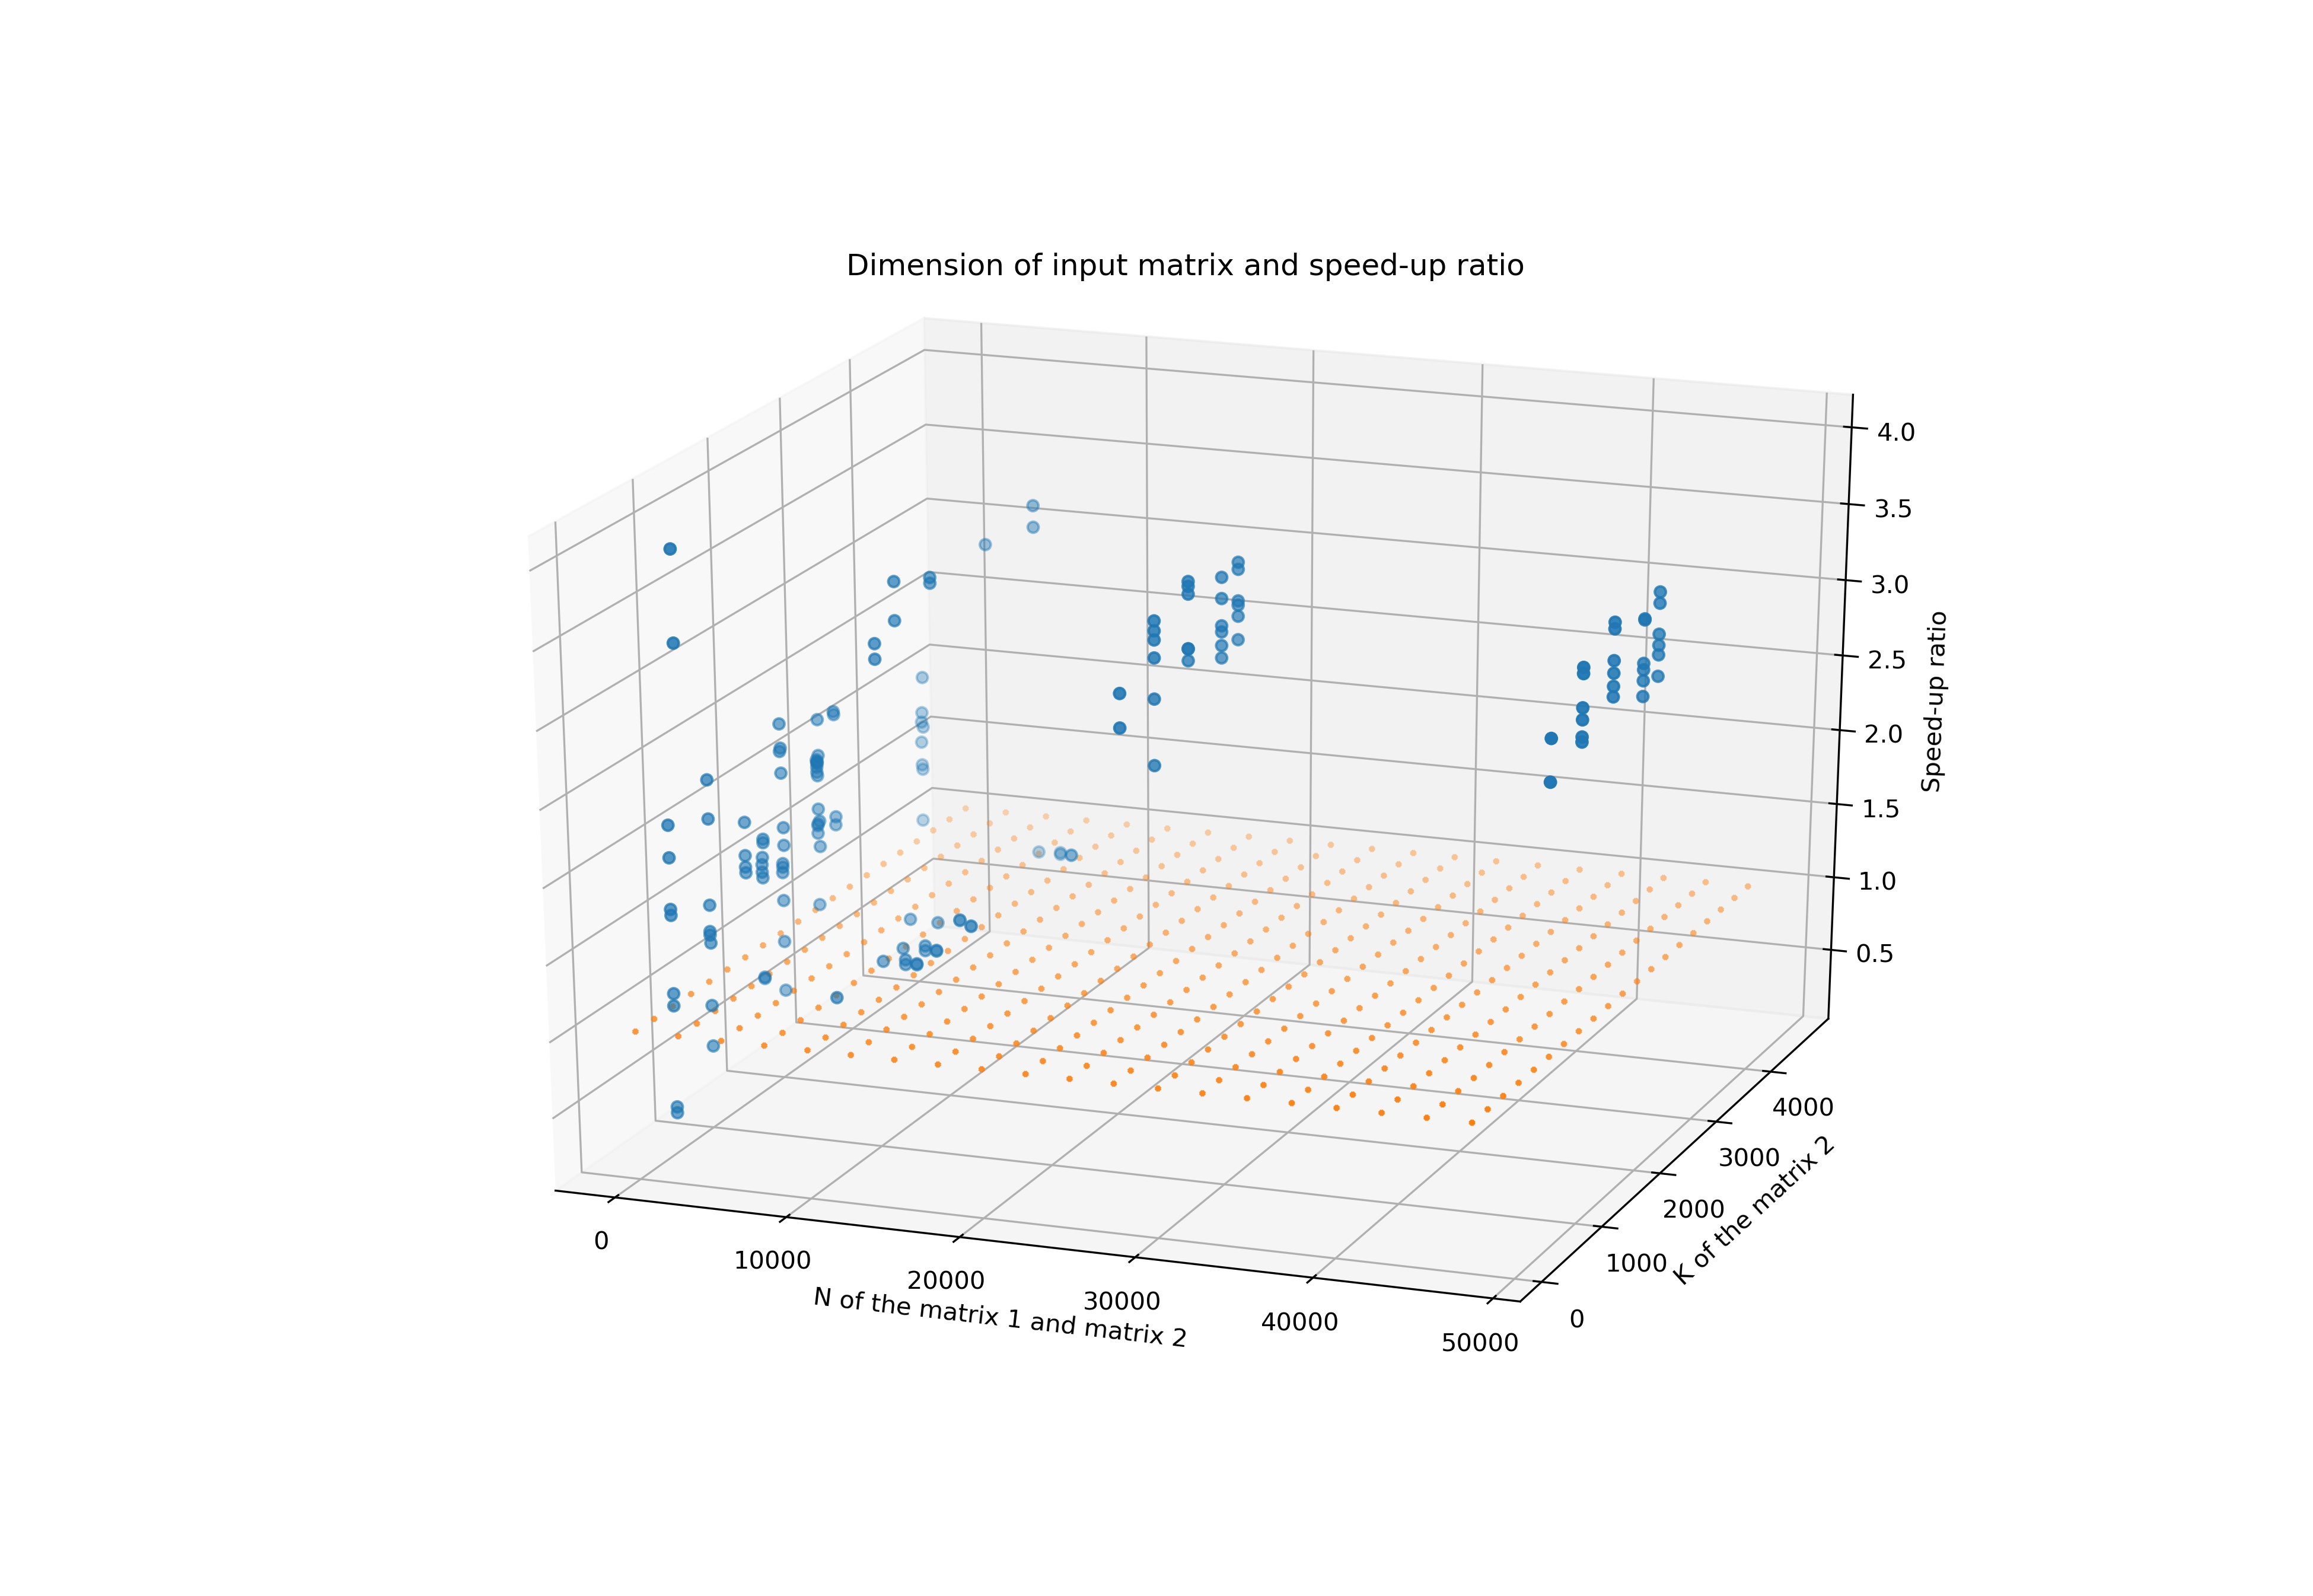
\includegraphics[height=7.2cm]{figures/GEMM_NK.jpg}\\
	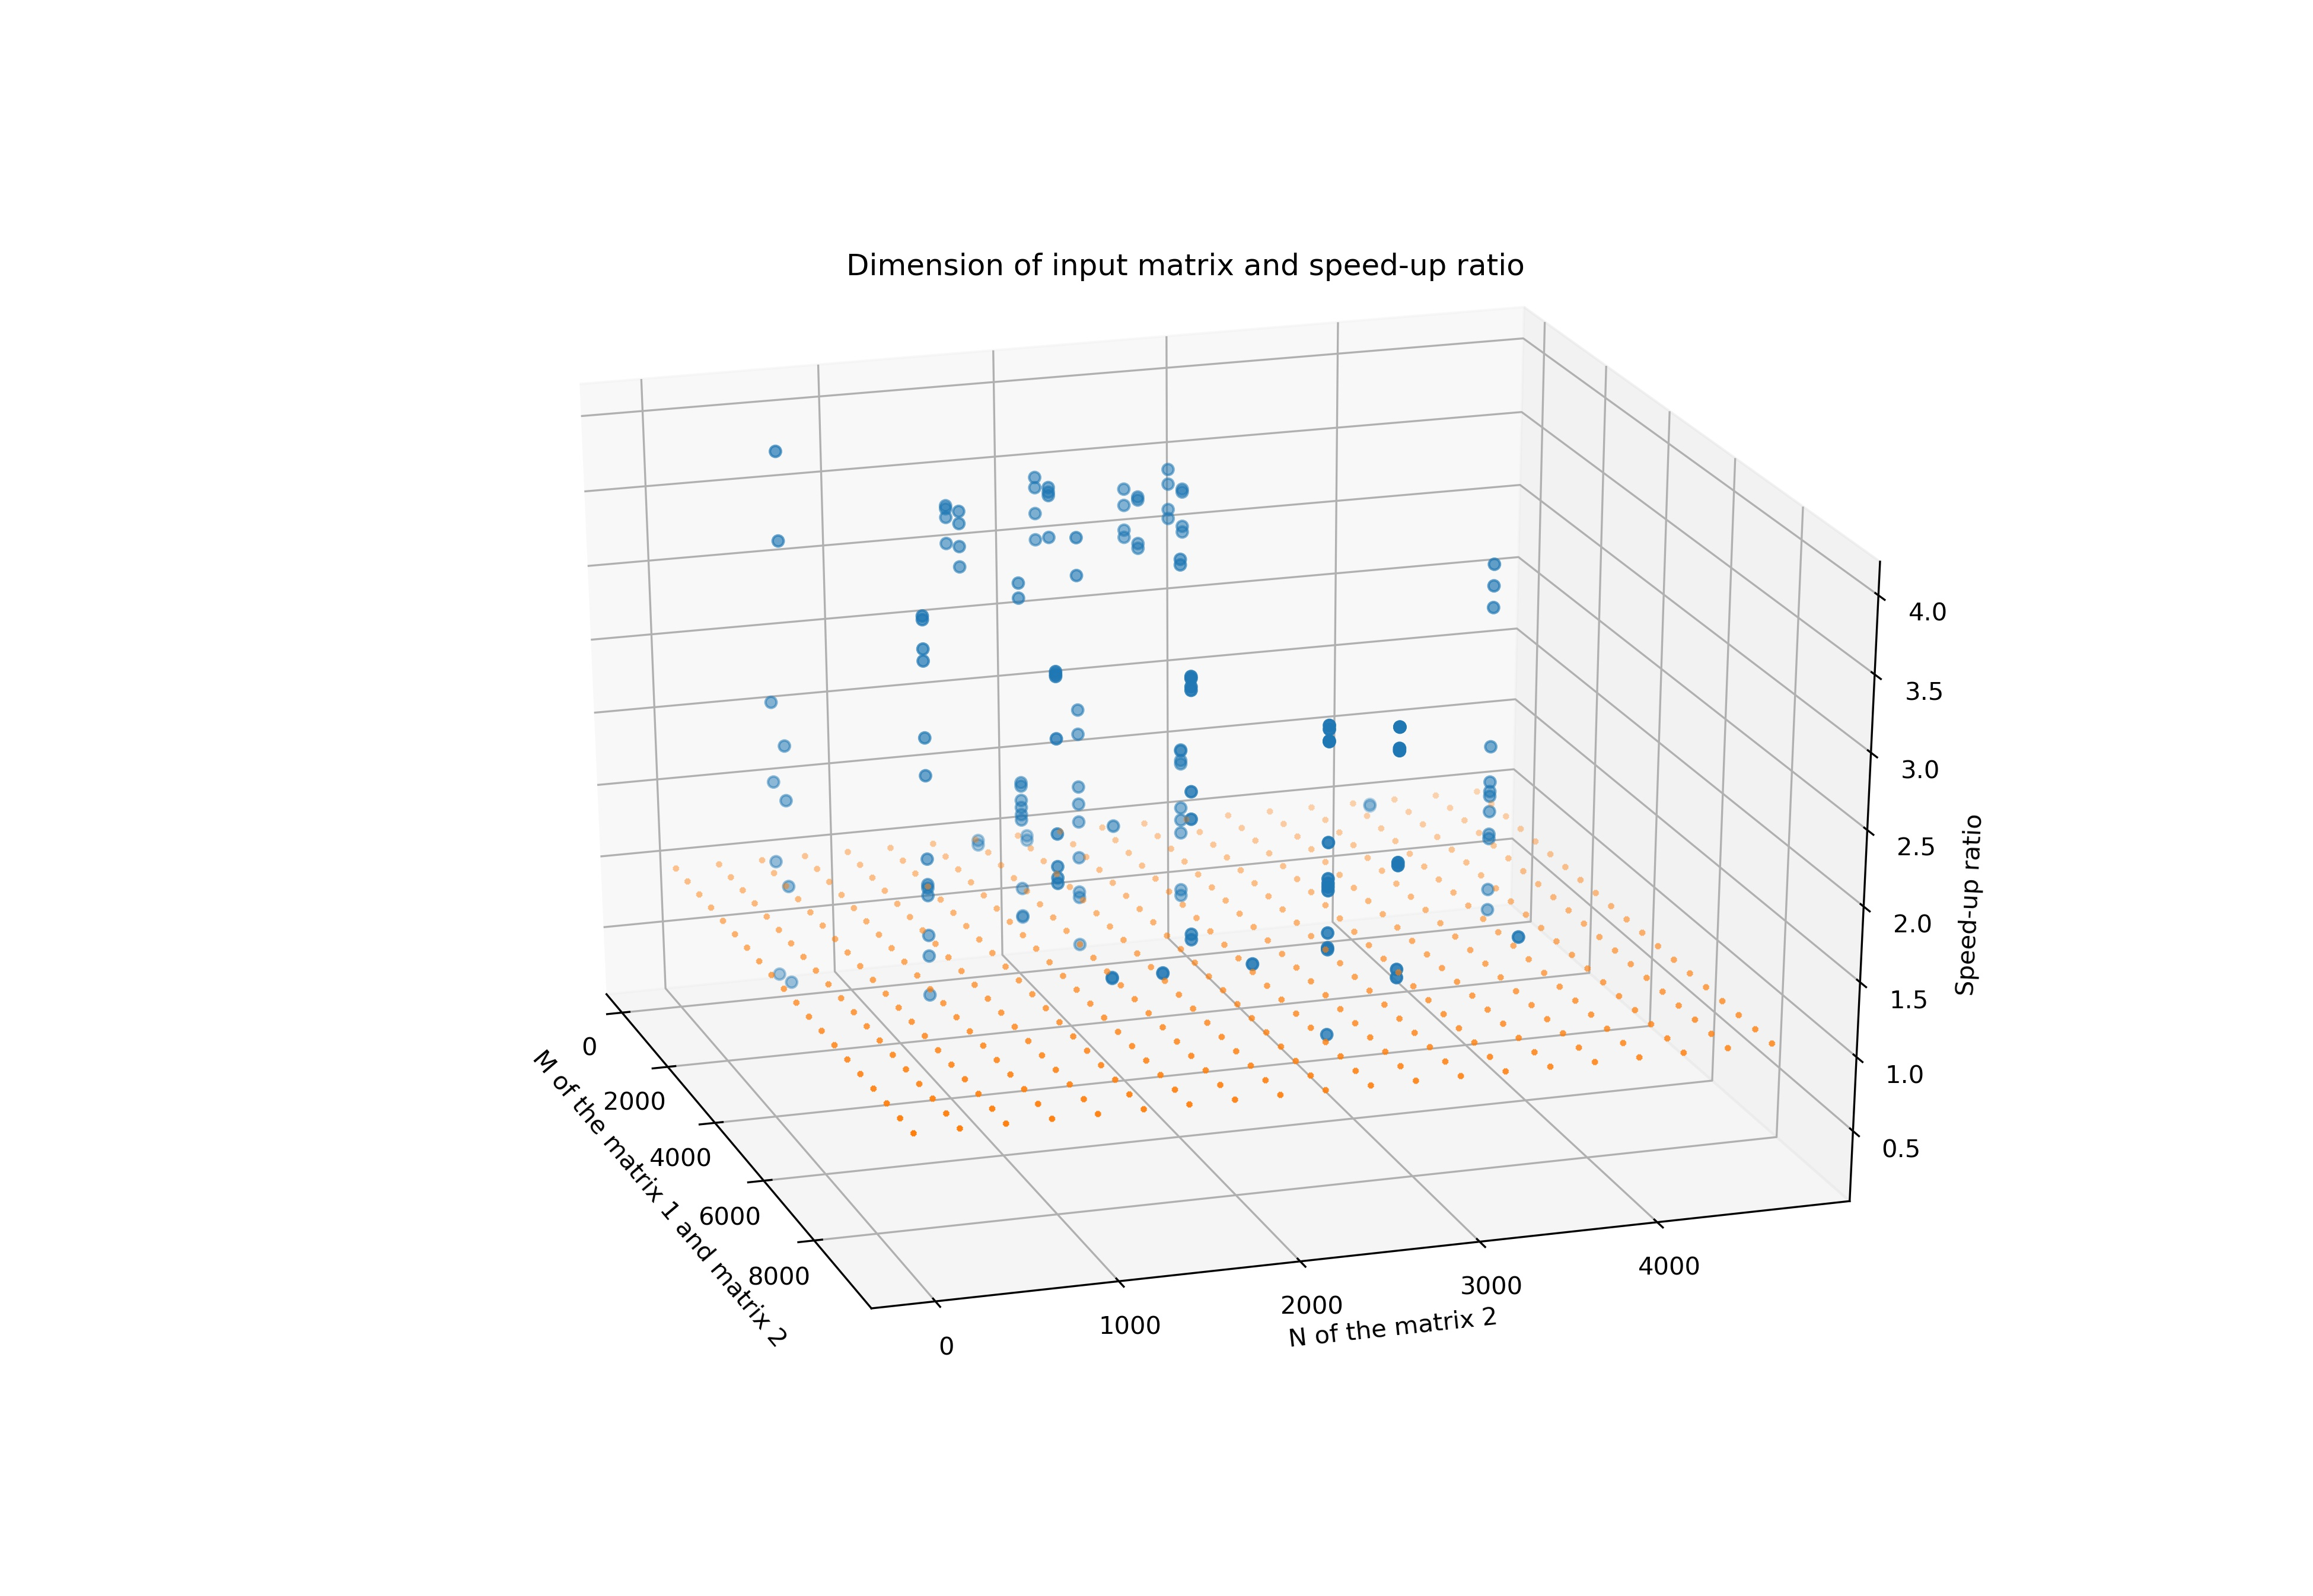
\includegraphics[height=7.2cm]{figures/GEMM_MN.jpg}
	\renewcommand{\thefigure}{\arabic{section}-\arabic{figure} }
	\renewcommand{\figurename}{图}
	\caption{输入矩阵维度与加速比的关系}
	\addtocounter{figure}{-1}
	\renewcommand{\thefigure}{\arabic{section}-\arabic{figure} }
	\renewcommand{\figurename}{Figure}
	\caption{Relationship of input matrix dimension and speed-up ratio}
	\label{Fig-MNKRatio}
\end{figure}
\begin{figure}
	\centering
	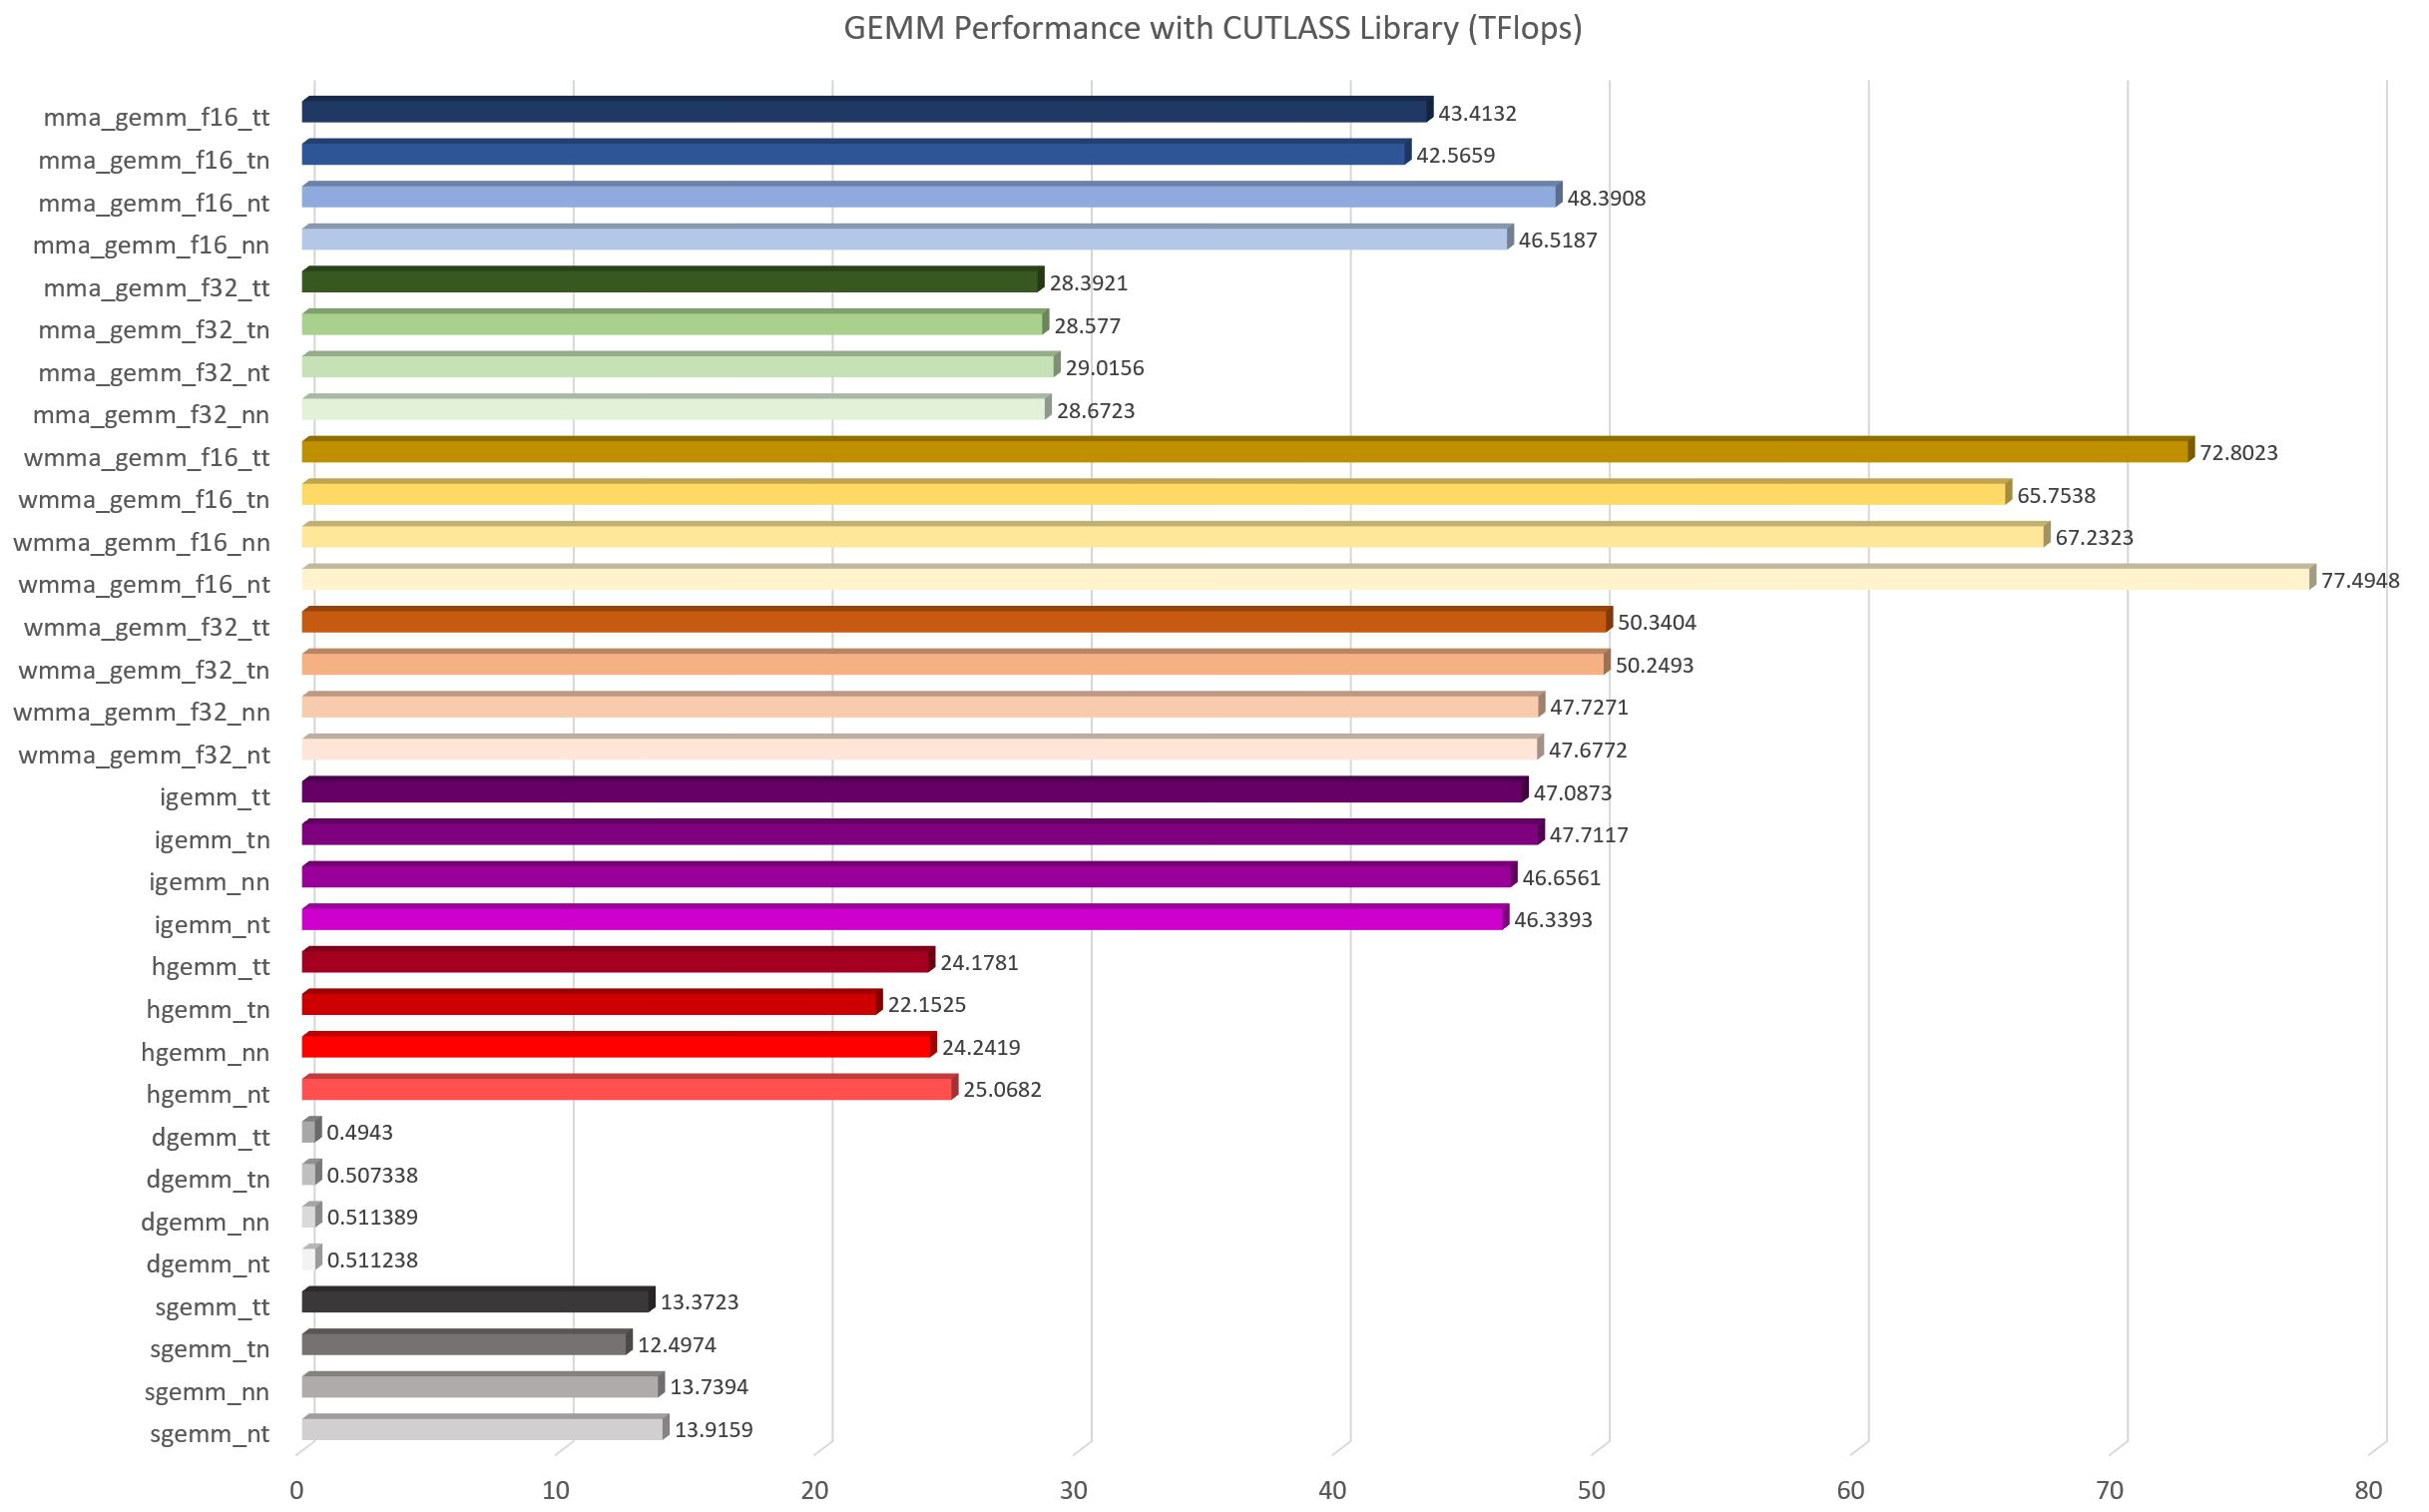
\includegraphics[width=15cm]{figures/CUTLASSGEMM.jpg}
	\renewcommand{\thefigure}{\arabic{section}-\arabic{figure} }
	\renewcommand{\figurename}{图}
	\caption{使用模板库测得的GEMM性能}
	\addtocounter{figure}{-1}
	\renewcommand{\thefigure}{\arabic{section}-\arabic{figure} }
	\renewcommand{\figurename}{Figure}
	\caption{GEMM Performance with CUTLASS}
	\label{Fig-GEMM-CUTLASS}
\end{figure}
\paragraph{结果分析}
\par 首先,本实验通过Nsight和nvprof的搭配对应用程序中包括API调用、核函数运行时间等运行时细节进行研究。图 \ref{Fig.GEMMPROFTF}和图 \ref{Fig.GEMMPROFNOTF}是开启和关闭张量核心的情况下,使用nvprof运行通用矩阵乘法应用所得到的报告,该报告主要侧重于API的调用、运行。由于本文关心的重点在GPU硬件,故仅截取硬件相关的API调用(API Call)部分。图中由左至右边分别代表API调用占比、运行总时长、调用次数、平均运行时长、最短运行时长、最长运行时长和API名称。
\begin{figure}
	\centering
	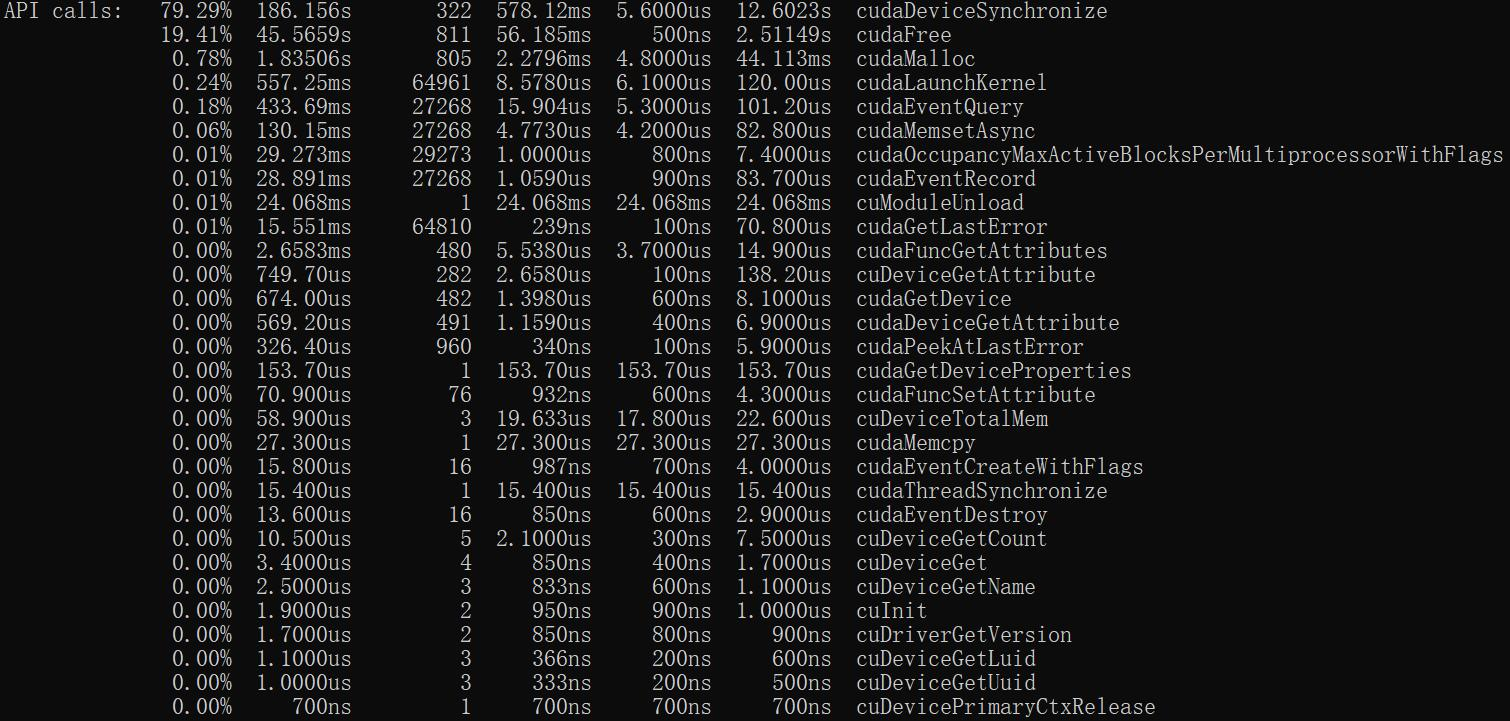
\includegraphics[width=15cm]{figures/GEMM-TF.jpg}
	\renewcommand{\thefigure}{\arabic{section}-\arabic{figure} }
	\renewcommand{\figurename}{图}
	\caption{开启张量核心下通用矩阵乘法运算的性能分析(API Calls)}
	\addtocounter{figure}{-1}
	\renewcommand{\thefigure}{\arabic{section}-\arabic{figure} }
	\renewcommand{\figurename}{Figure}
	\caption{Performance analysis of GEMM with Tensor Core On (API Calls)}
	\label{Fig.GEMMPROFTF}
\end{figure}
\begin{figure}
	\centering
	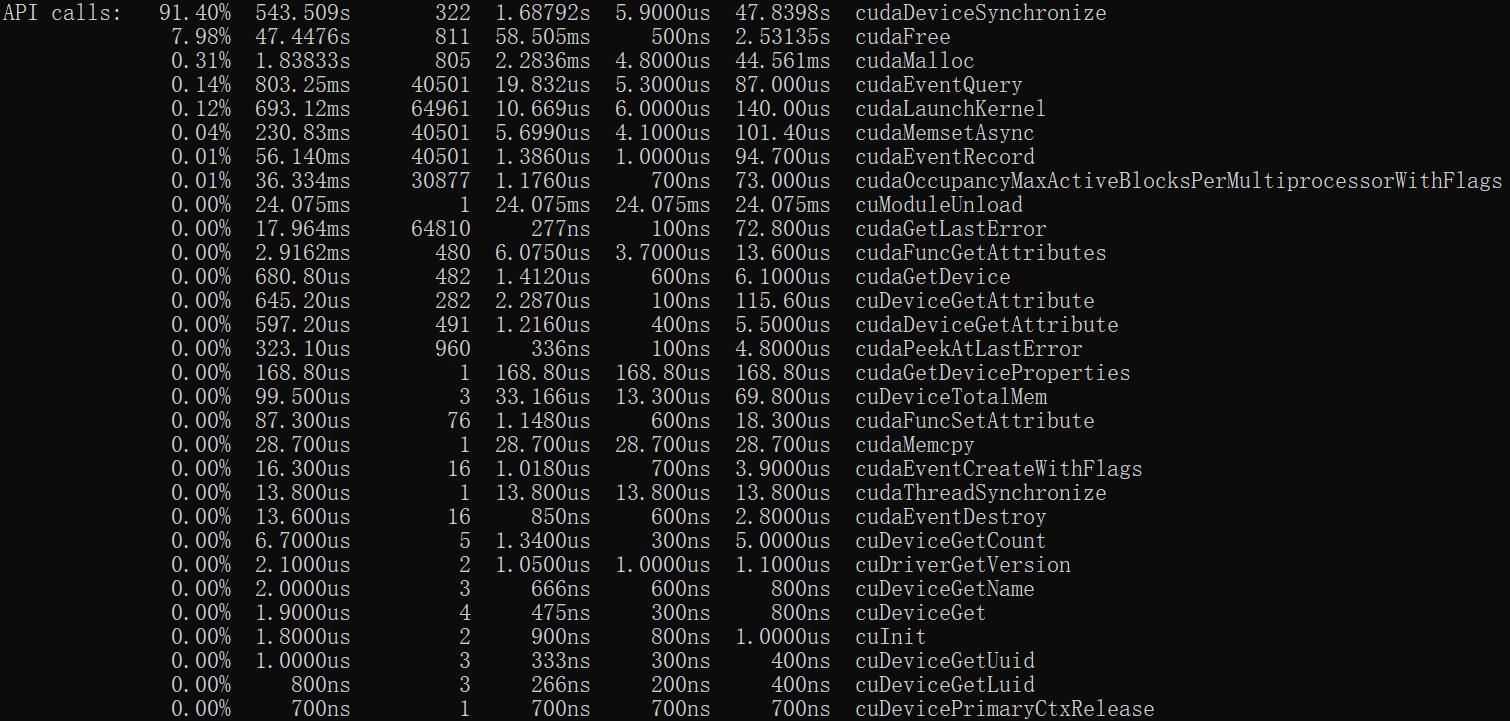
\includegraphics[width=15cm]{figures/GEMM-NOTF.jpg}
	\renewcommand{\thefigure}{\arabic{section}-\arabic{figure} }
	\renewcommand{\figurename}{图}
	\caption{关闭张量核心下通用矩阵乘法运算的性能分析(API Calls)}
	\addtocounter{figure}{-1}
	\renewcommand{\thefigure}{\arabic{section}-\arabic{figure} }
	\renewcommand{\figurename}{Figure}
	\caption{Performance analysis of GEMM with Tensor Core Off (API Calls)}
	\label{Fig.GEMMPROFNOTF}
\end{figure}
\par 根据nvprof生成的报告,可以看出在开启张量核心的情况下,用于设备上线程束同步的API:cudaDeviceSynchronize(),无论是在运行总时长还是调用占比中都显著小于不开启张量核心的情况。另外用于开启内核运行和异步访存的API的调用次数在开启张量核心时都明显小于不开启张量核心的情况。可见开启张量核心后,由于原先需要多条点积指令的矩阵乘法运算被合并为仅用一条wmma指令替代,其计算更加密集、设备同步更少,故性能提升明显。表 \ref{table-时钟周期}显示了根据GPGPU-SIM测得的张量核心相关指令与一般点积运算指令所需要的运行周期数,以及相应开启内核(Launch Kernel)指令所需的运行周期数,在关闭张量核心时,进行矩阵乘加或是通过多条浮点指令、或是通过多条ALU指令(idp4a)实现的,而开启张量核心后则直接通过wmma指令实现,如图 \ref{Fig.HMMASASS}所示,图中为硬件代码(SASS),wmma经过编译会生成若干条hmma指令,图中hmma指令的动作为:以$ m=8,n=8,k=4 $为最小粒度,在FP32精度E8M10存储方式的浮点数上进行运算。根据指令运行周期级别的数据可以看出使用张量核心相关指令(wmma)不仅能极大减少计算所花费的时间,用于开启内核、上下文切换的时间也会显著减少。
\begin{table}
	\centering
	\renewcommand{\thetable}{\arabic{section}-\arabic{table} }
	\renewcommand{\tablename}{表}
	\caption{GPGPU-SIM测得的各指令运行所需时钟周期(图灵架构)}
	\addtocounter{table}{-1}
	\renewcommand{\thetable}{\arabic{section}-\arabic{table} }
	\renewcommand{\tablename}{Table}
	\caption{Clock cycle the instructions will cost based on GPGPU-SIM(Turing Arch)}
	\begin{tabular}{cc}
		\toprule
		指令、操作类型	&	周期\\
		\midrule
		FMA(Float point Multiply Accumulation) @ FP32 & 4 \\
		FMA @ FP64	&	8\\
		WMMA(Warp-level Matrix Multiply Accumulation)@FP16 & 8\\
		ALU 	&	4\\
		MIO(内存访问) & 16-20\\
		TRAP(内核陷阱) & 77-92\\
		L1缓存未命中 & 139-167\\
		\bottomrule
	\end{tabular} \label{table-时钟周期} \\
	
	$ * $因硬件运行时存在随机性,故测得时钟周期为在基于图灵架构的GPGPU-SIM上运行后计算得出。
\end{table}
\begin{figure}
	\centering
	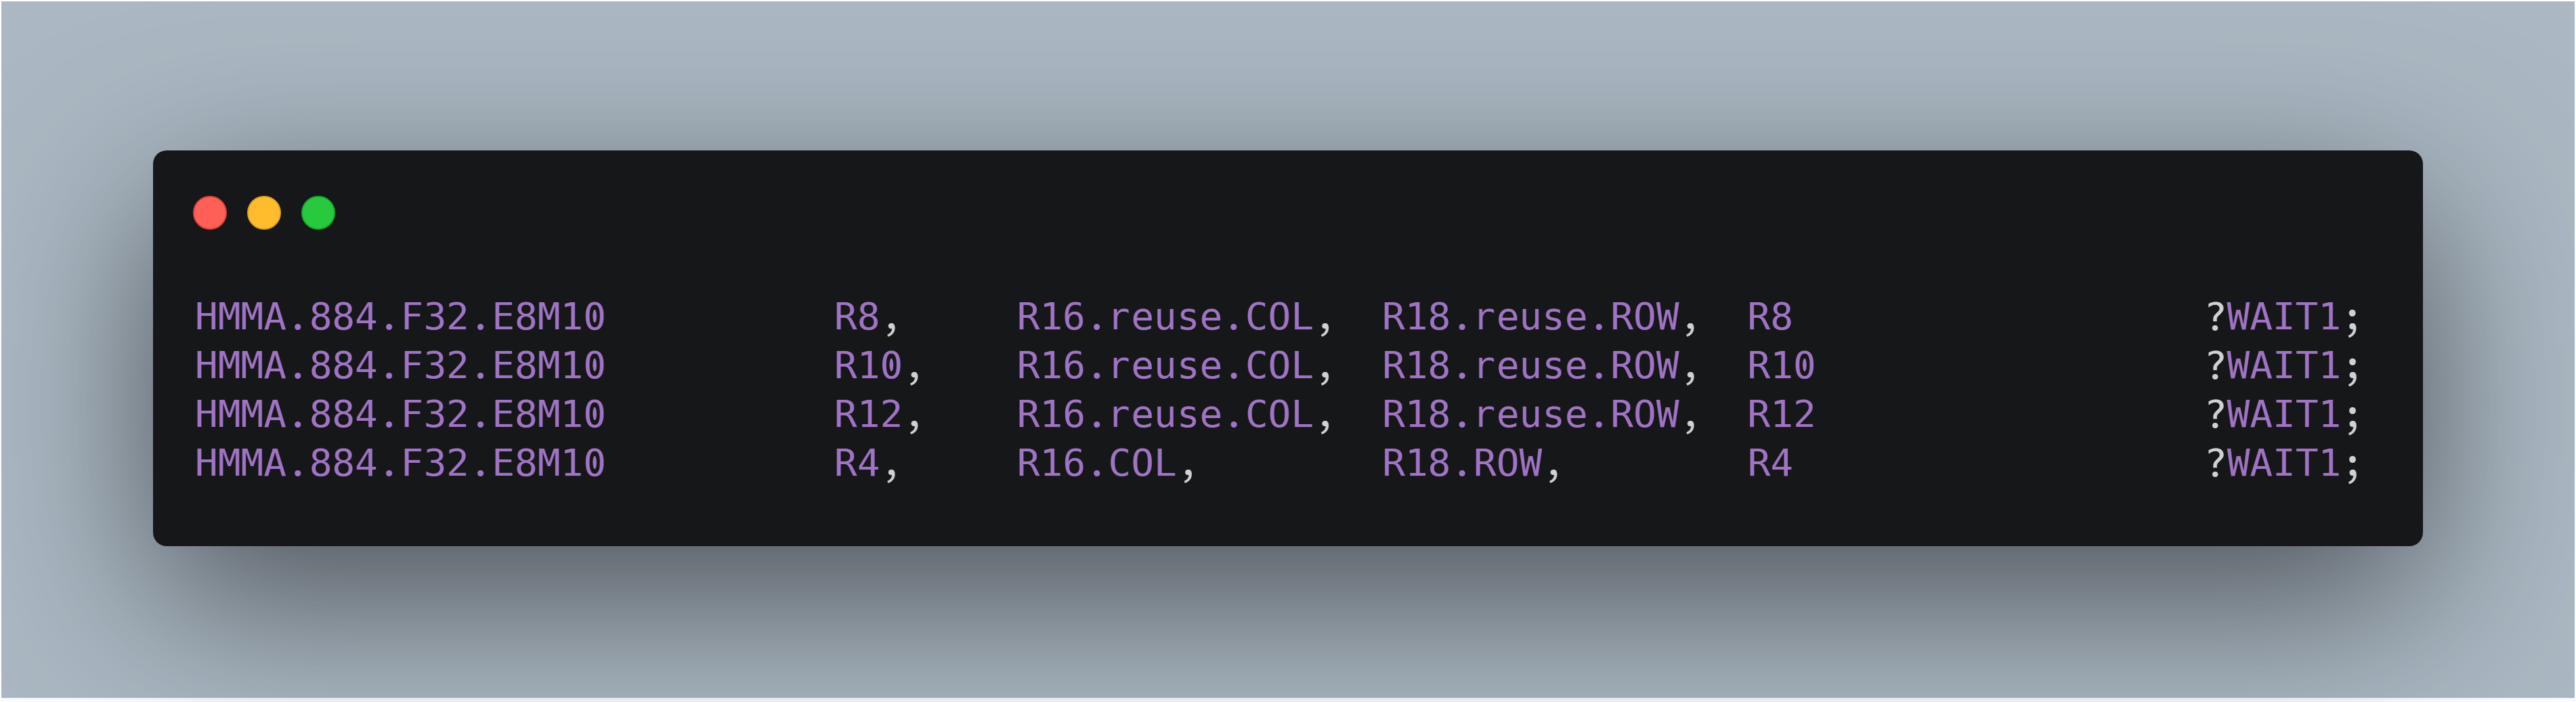
\includegraphics[width=15cm]{figures/HMMASASS.jpg}
	\renewcommand{\thefigure}{\arabic{section}-\arabic{figure} }
	\renewcommand{\figurename}{图}
	\caption{一段由wmma指令编译出的机器指令}
	\addtocounter{figure}{-1}
	\renewcommand{\thefigure}{\arabic{section}-\arabic{figure} }
	\renewcommand{\figurename}{Figure}
	\caption{Part of SASS code complied from PTX code: wmma}
	\label{Fig.HMMASASS}
\end{figure}
\par 图 \ref{Fig.GEMMSIGHTTF}和图 \ref{Fig.GEMMSIGHTNOTF}则是开启和关闭张量核心的情况下,使用Nsight运行通用矩阵乘法应用所得到的报告,该报告主要侧重于上下文切换、线程调度等信息。在这些信息中本实验重点关注线程就绪(Ready Thread)和上下文切换(Context Switch)两部分。

\begin{figure}
	\centering
	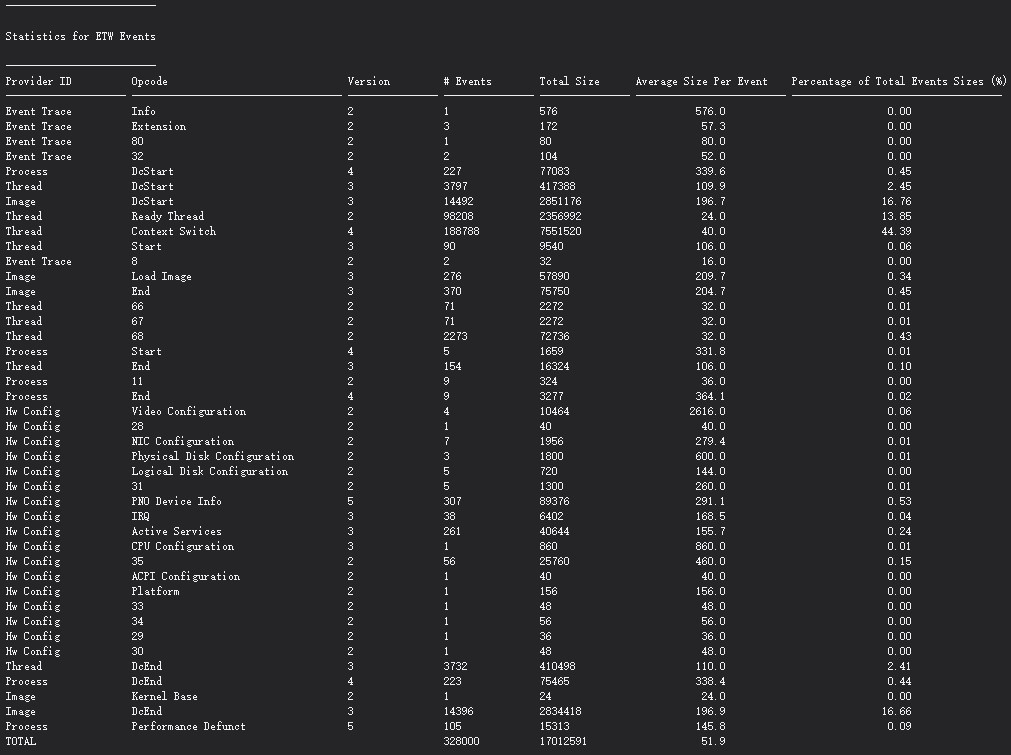
\includegraphics[width=15cm,height=10cm]{figures/GEMMSIGHTTF.jpg}
	\renewcommand{\thefigure}{\arabic{section}-\arabic{figure} }
	\renewcommand{\figurename}{图}
	\caption{开启张量核心下通用矩阵乘法运算的性能分析(上下文切换)}
	\addtocounter{figure}{-1}
	\renewcommand{\thefigure}{\arabic{section}-\arabic{figure} }
	\renewcommand{\figurename}{Figure}
	\caption{Performance analysis of GEMM with Tensor Core On (Context Switch)}
	\label{Fig.GEMMSIGHTTF}
\end{figure}
\begin{figure}
	\centering
	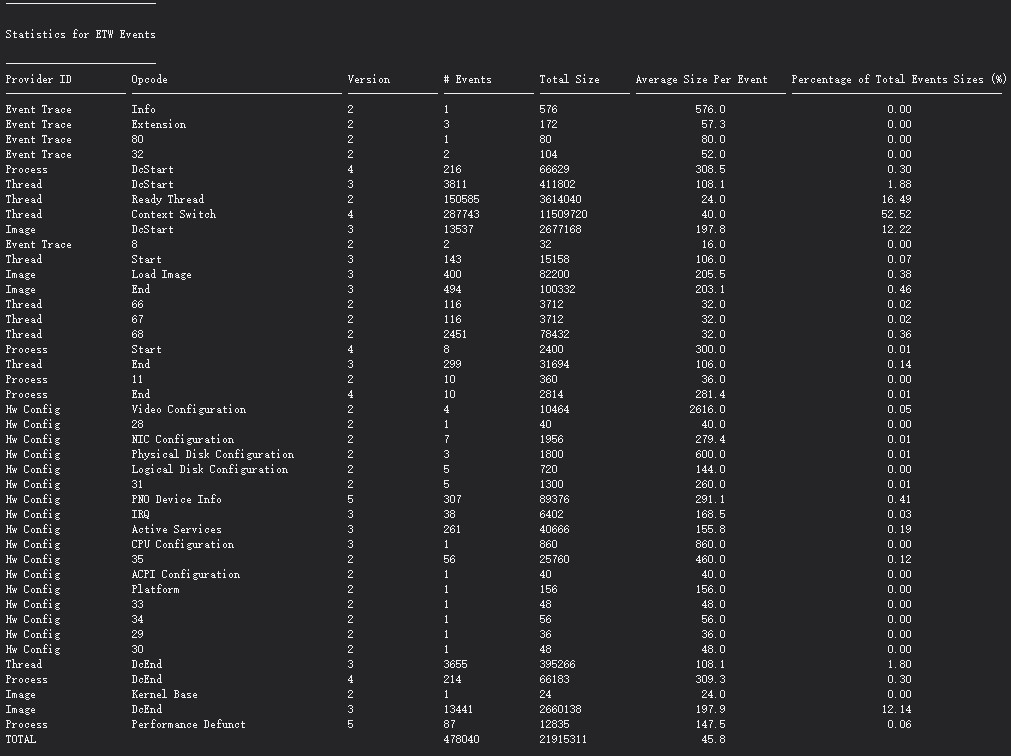
\includegraphics[width=15cm,height=10cm]{figures/GEMMSIGHTNOTF.jpg}
	\renewcommand{\thefigure}{\arabic{section}-\arabic{figure} }
	\renewcommand{\figurename}{图}
	\caption{关闭张量核心下通用矩阵乘法运算的性能分析(上下文切换)}
	\addtocounter{figure}{-1}
	\renewcommand{\thefigure}{\arabic{section}-\arabic{figure} }
	\renewcommand{\figurename}{Figure}
	\caption{Performance analysis of GEMM with Tensor Core Off (Context Switch)}
	\label{Fig.GEMMSIGHTNOTF}
\end{figure}
\par 根据Nsight生成的报告,可以看出无论是否开启张量核心,其上下文切换仍然是一笔较大的开销。正如上文提到的,在GPU上进行上下文切换,其寄存器可以简单地通过更改寄存器文件指针保存/还原,然而上下文切换所需要做的清空流水线等工作还是无法被省略,造成较大的开销。相比较而言开启张量核心的应用在上下文切换中的开销下降了10\%左右,而因为就算不使用张量核心, $ 4\times4 $规模的混合矩阵运算也能使用点积指令在16个周期内完成,故应用中运算开销相对于上下文切换、加载内核映像的工作占用资源较小。且使用张量核心的应用中硬件中断(IRQ)占比也较小,说明使用张量核心不仅在运算速度上有极大提升,在与外围设备数据交换,缓存读取、命中等方面都有较大优势。当然,因计算优势在缓存读取、命中等方面体现,故输入数据的“形状”能否符合张量的硬件特性变得尤为重要。
\par 在上文的实验中,可以看出矩阵乘加运算中,两输入矩阵共享的维度$ K $对性能影响较为显著。在$ M\times N$ 的结果矩阵中,每个单元格都是由$ 1\times K $的矩阵与$ K\times 1 $矩阵相乘,这个运算将被拆分并分发给张量核心进行处理,那么在这一步,若$ K $无法被张量核心正好拆分,则会引发一个数据缺失,进而造成硬件中断,旨在从共享/全局内存获取新的数据以拼成完整的可以交予张量核心进行处理的单元。若没有这种数据则调用传统运算核心进行运算。那么张量核心硬件上是以$ 4\times 4 $作为计算单元,调度时以$ 16\times 16 $作为调度单元,那么隐含的就要求$ K $能被恰好拆分为16或4,到此,我们根据官方文档、硬件架构做出了猜想,根据下面两张图中的实验数据,我们将对这个猜想进行验证。图 \ref{Fig-PerfGemmByratio}左侧为按照开启与关闭张量核心情况下的半精度混合矩阵运算的加速比进行排序,并记录下实验编号的顺序,然后使用记录下的实验编号的顺序对单精度混合矩阵运算的实验结果进行排序得到右侧图表(右侧图表并不是按照单精度混合矩阵运算实验的加速比排序,而是根据基于加速比排序后的半精度混合矩阵运算实验得到的实验编号的顺序排序)。两张图中的加速比可被分为三段:加速比低于1、加速比介于1-2.5之间和加速比大于3的部分,且两图中突变坐标吻合,故可以推测与精度无关、在硬件上张量核心对于输入操作数的形状较为敏感。
\begin{figure}
	\centering
	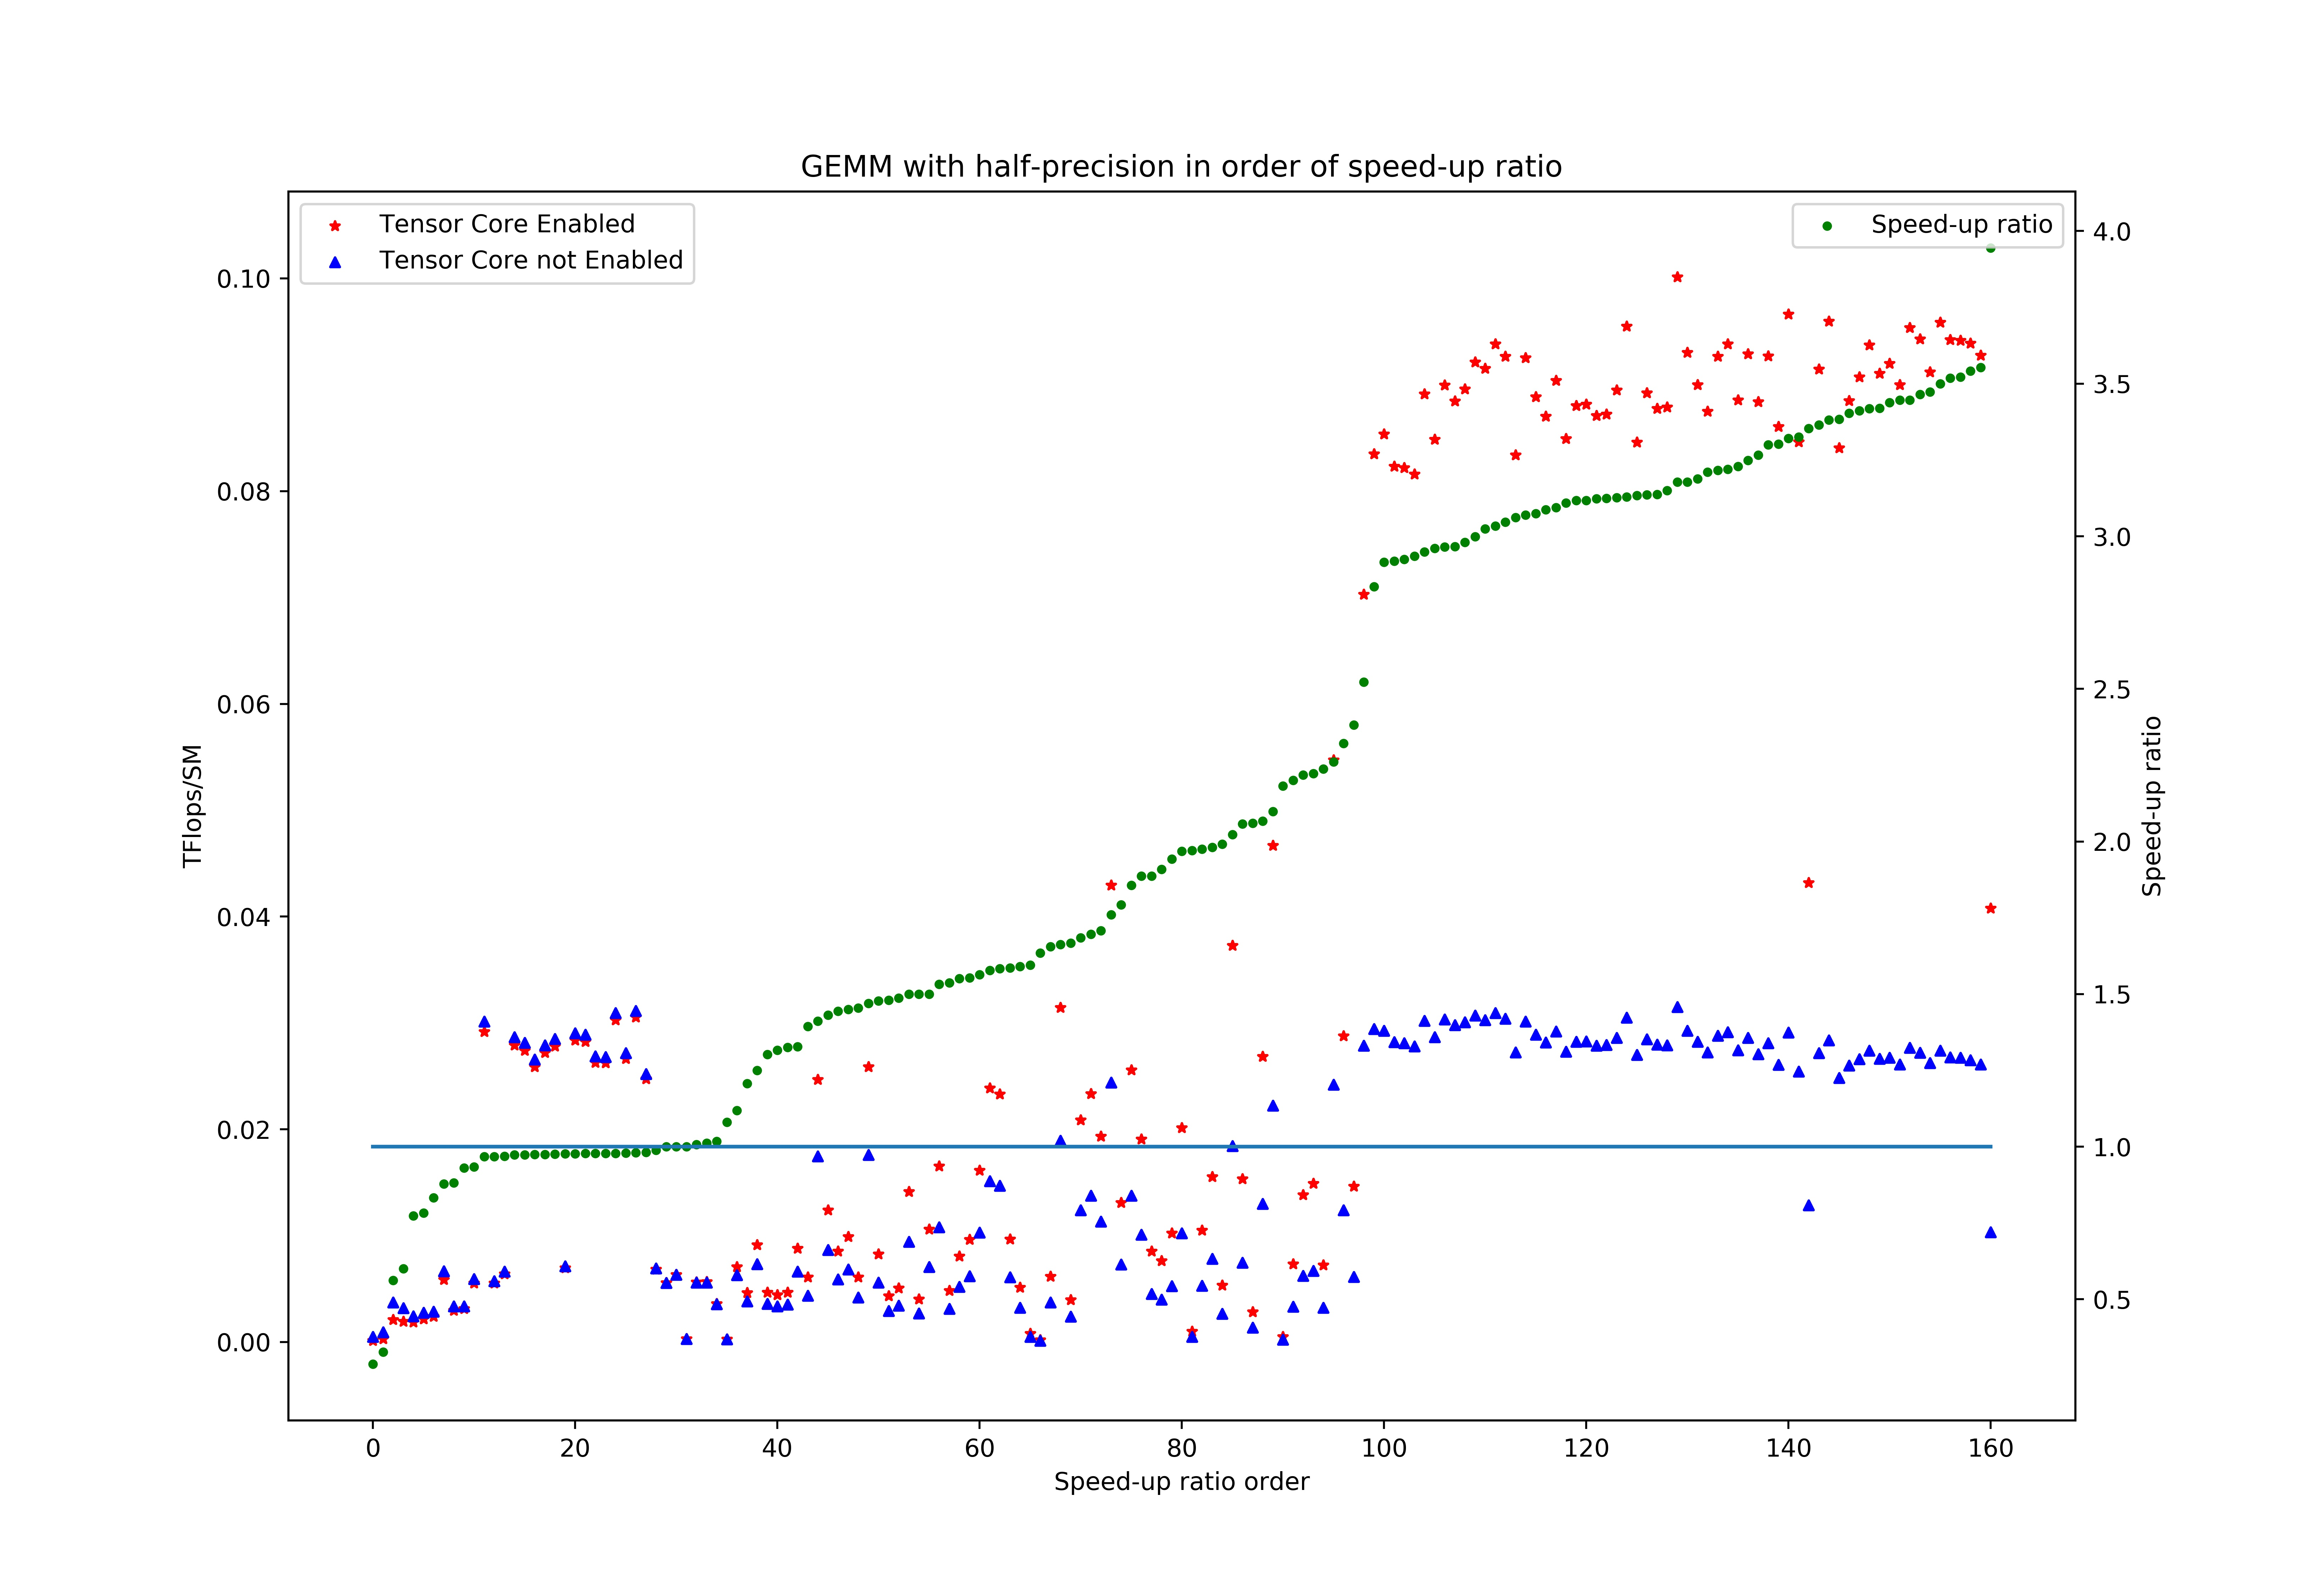
\includegraphics[width=15cm]{figures/GEMM-Half-TF-Byratio.jpg}\\
	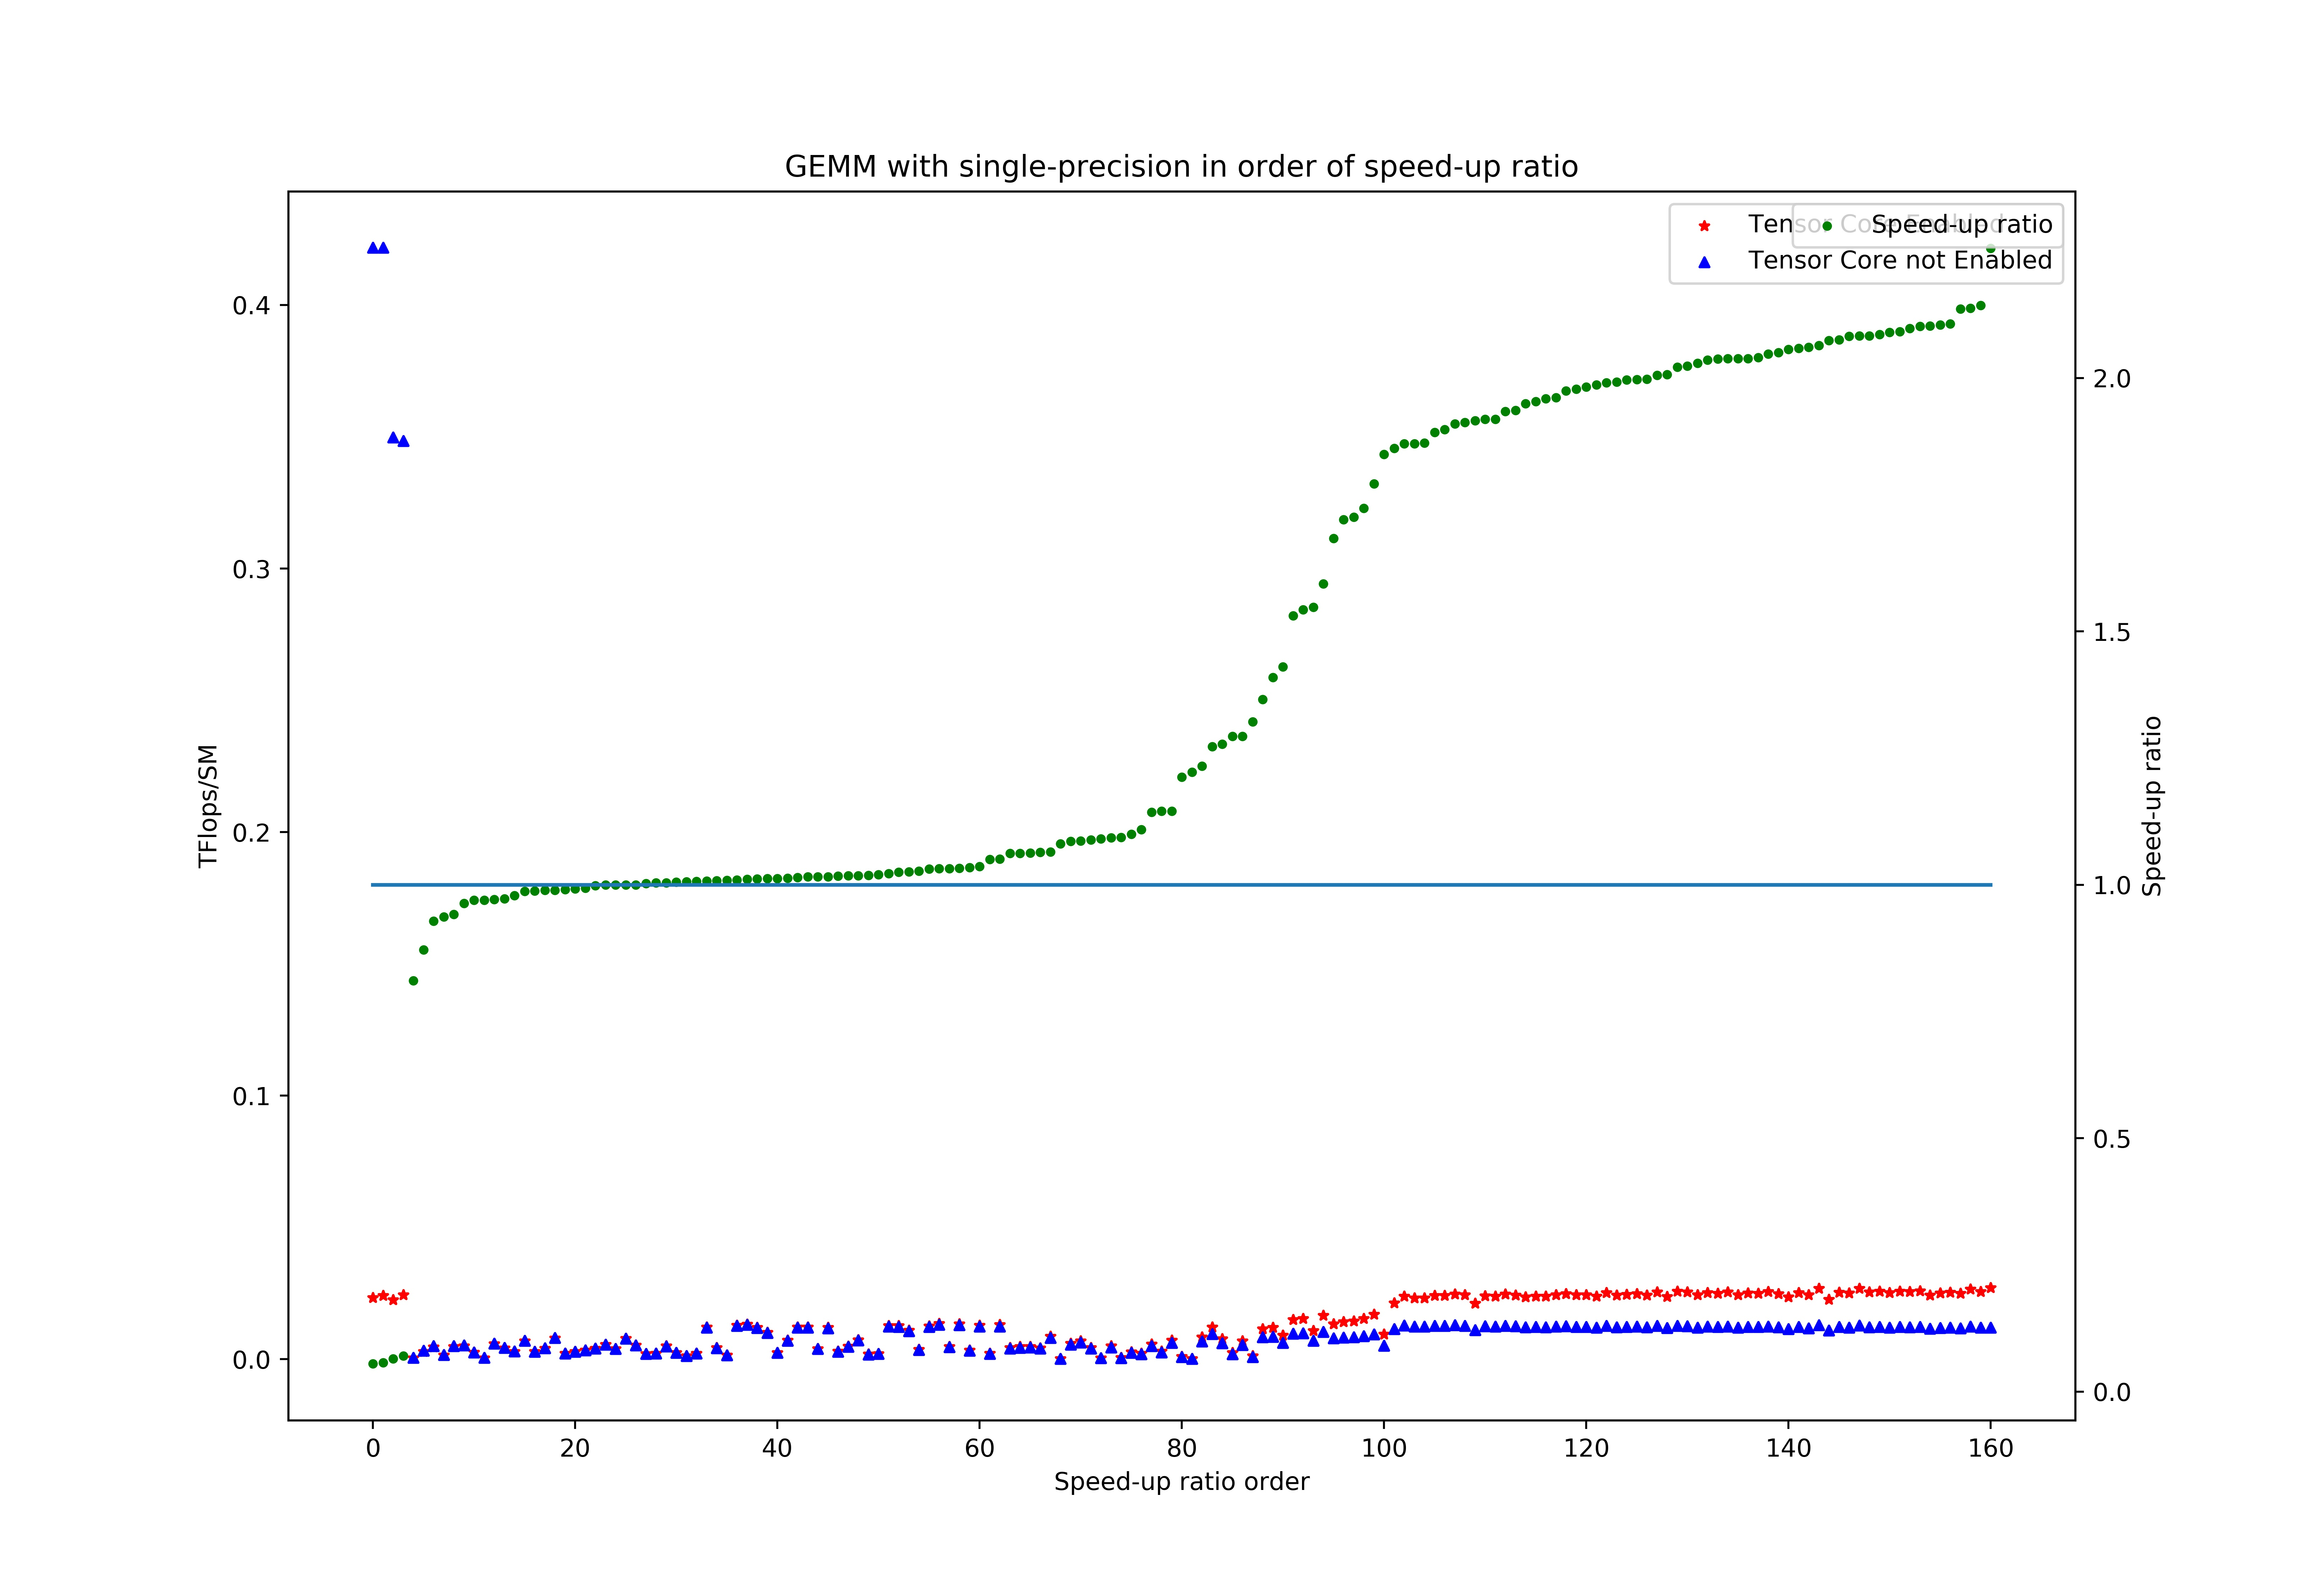
\includegraphics[width=15cm]{figures/GEMM-Single-TF-Byratio.jpg}
	\renewcommand{\thefigure}{\arabic{section}-\arabic{figure} }
	\renewcommand{\figurename}{图}
	\caption{半精度/单精度GEMM性能(按加速比排序)}
	\addtocounter{figure}{-1}
	\renewcommand{\thefigure}{\arabic{section}-\arabic{figure} }
	\renewcommand{\figurename}{Figure}
	\caption{Performance of GEMM at Half and Single (Sorted by speed-up ratio)}
	\label{Fig-PerfGemmByratio}
\end{figure}
\par 图 \ref{Fig-PerfGemmByratioTri}中根据实验中输入矩阵共享的维度$ k $对加速比进行着色。可见无法被8整除的测试样例的加速比较低,接近1;而能够被8整除的测试样例大部分都能被张量核心有效地加速;而随着$ K $值的上升,加速比也呈现上升趋势。结合GPU实际在线程调度中的特征,以及中间代码(PTX)中给出的子矩阵分割形状参数,如图 \ref{Fig.WMMADOC}所示(图中wmma指令为跨线程束矩阵乘加,而mma则非跨线程束),在实际使用中应尽量确保输入矩阵共享的维度$ K $能够被8整除,且最好为32的倍数;且尽量不要使用太“扁”或太“长”的矩阵作为输入。
\begin{figure}
	\centering
	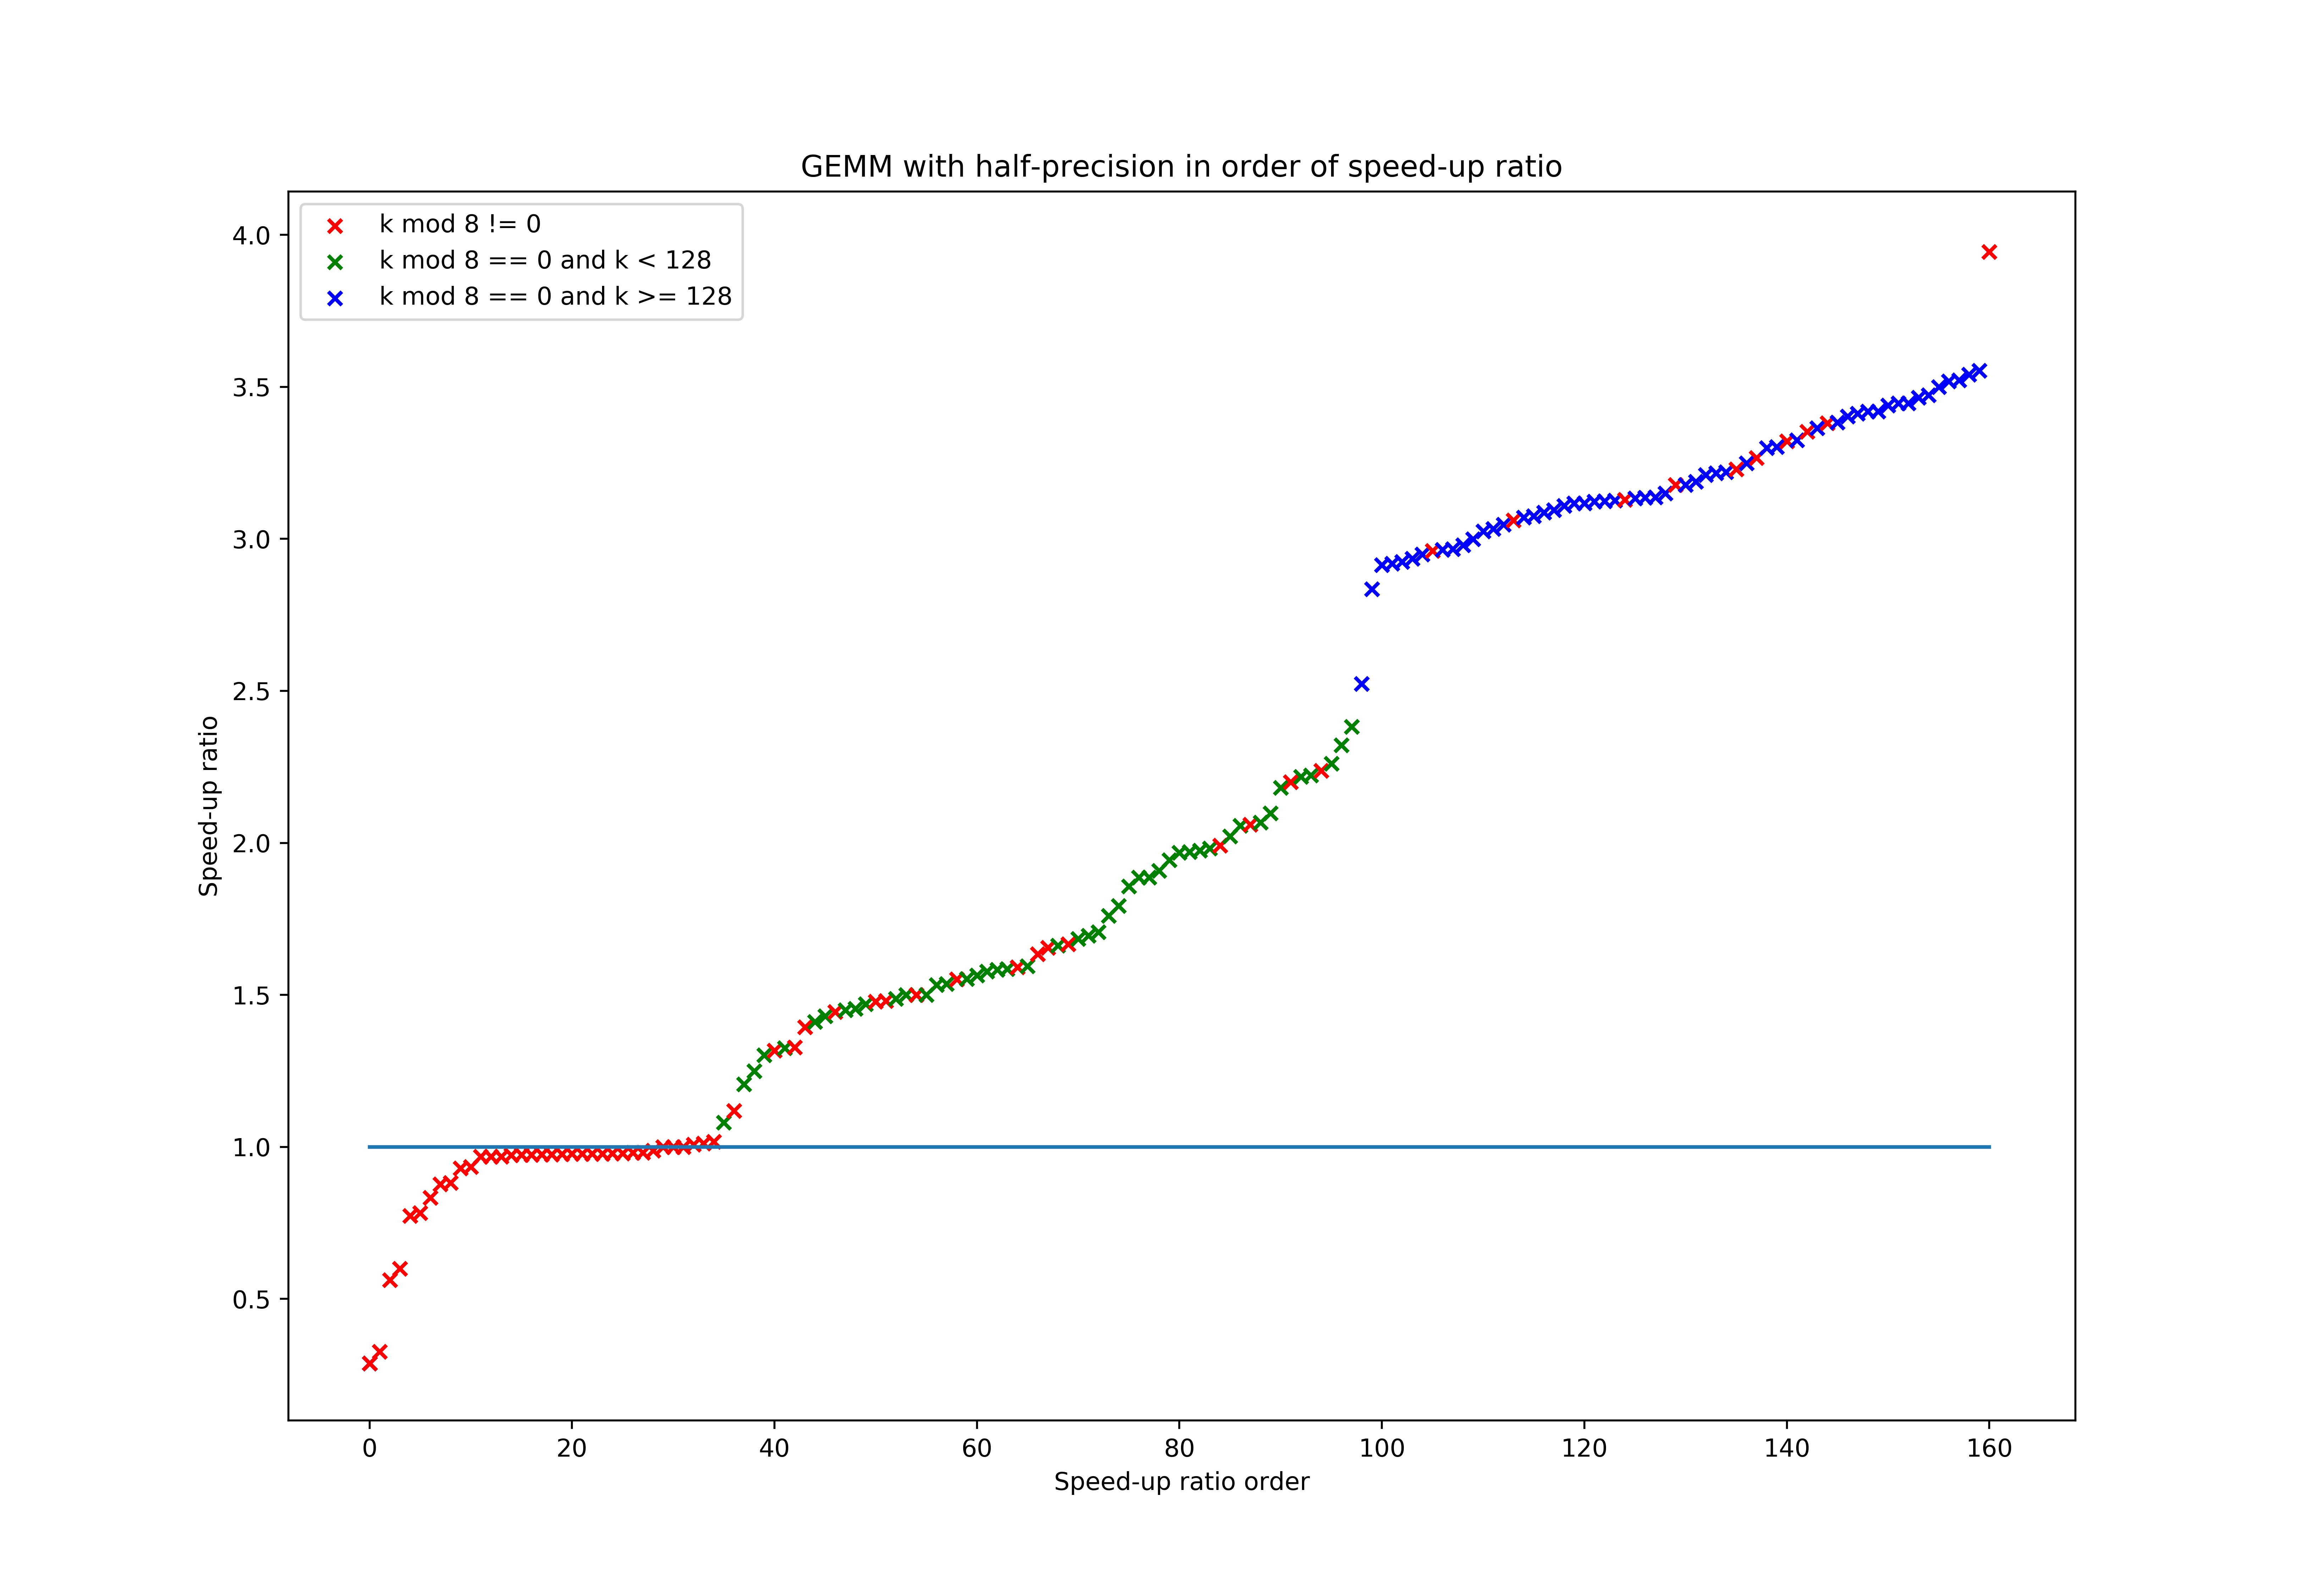
\includegraphics[width=15cm]{figures/GEMM-Half-TF-Byratio-Tri.jpg}\\
	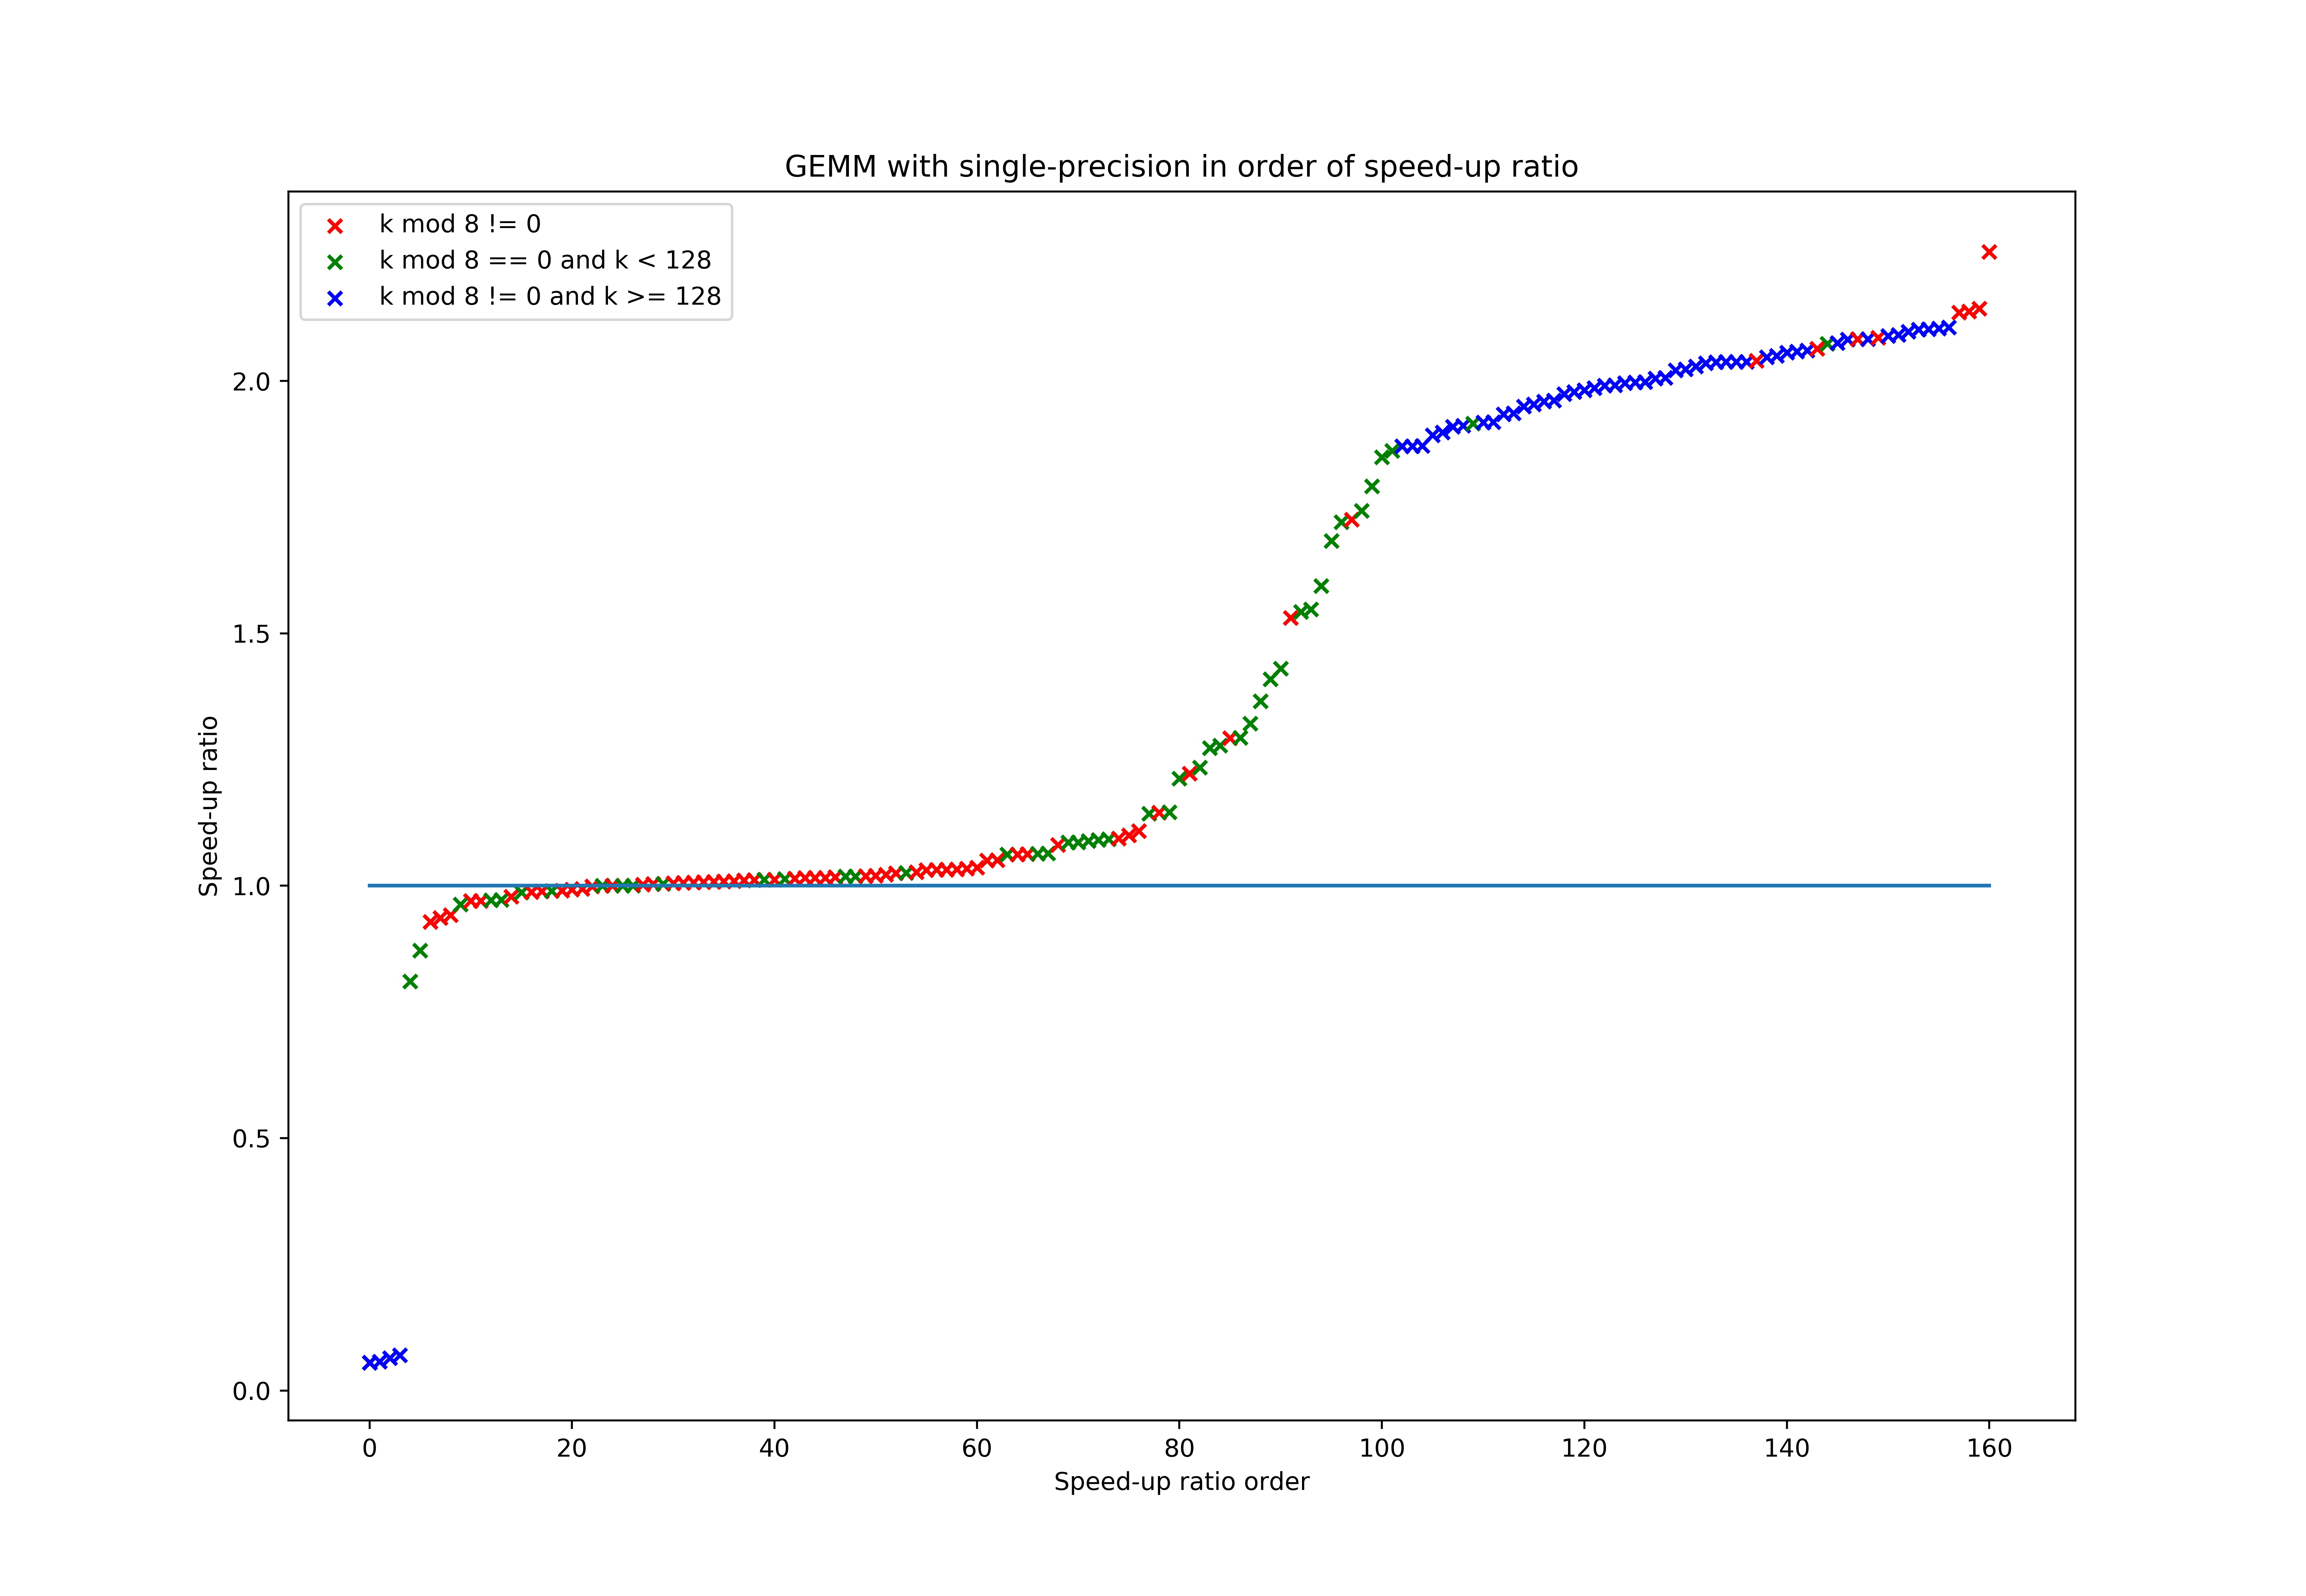
\includegraphics[width=15cm]{figures/GEMM-Single-TF-Byratio-Tri.jpg}
	\renewcommand{\thefigure}{\arabic{section}-\arabic{figure} }
	\renewcommand{\figurename}{图}
	\caption{半精度/单精度GEMM性能(按加速比排序,根据维度K特征着色)}
	\addtocounter{figure}{-1}
	\renewcommand{\thefigure}{\arabic{section}-\arabic{figure} }
	\renewcommand{\figurename}{Figure}
	\caption{Performance of GEMM at Half and Single (Sorted by speed-up ratio, colored with feature of K)}
	\label{Fig-PerfGemmByratioTri}
\end{figure}
\begin{figure}
	\centering
	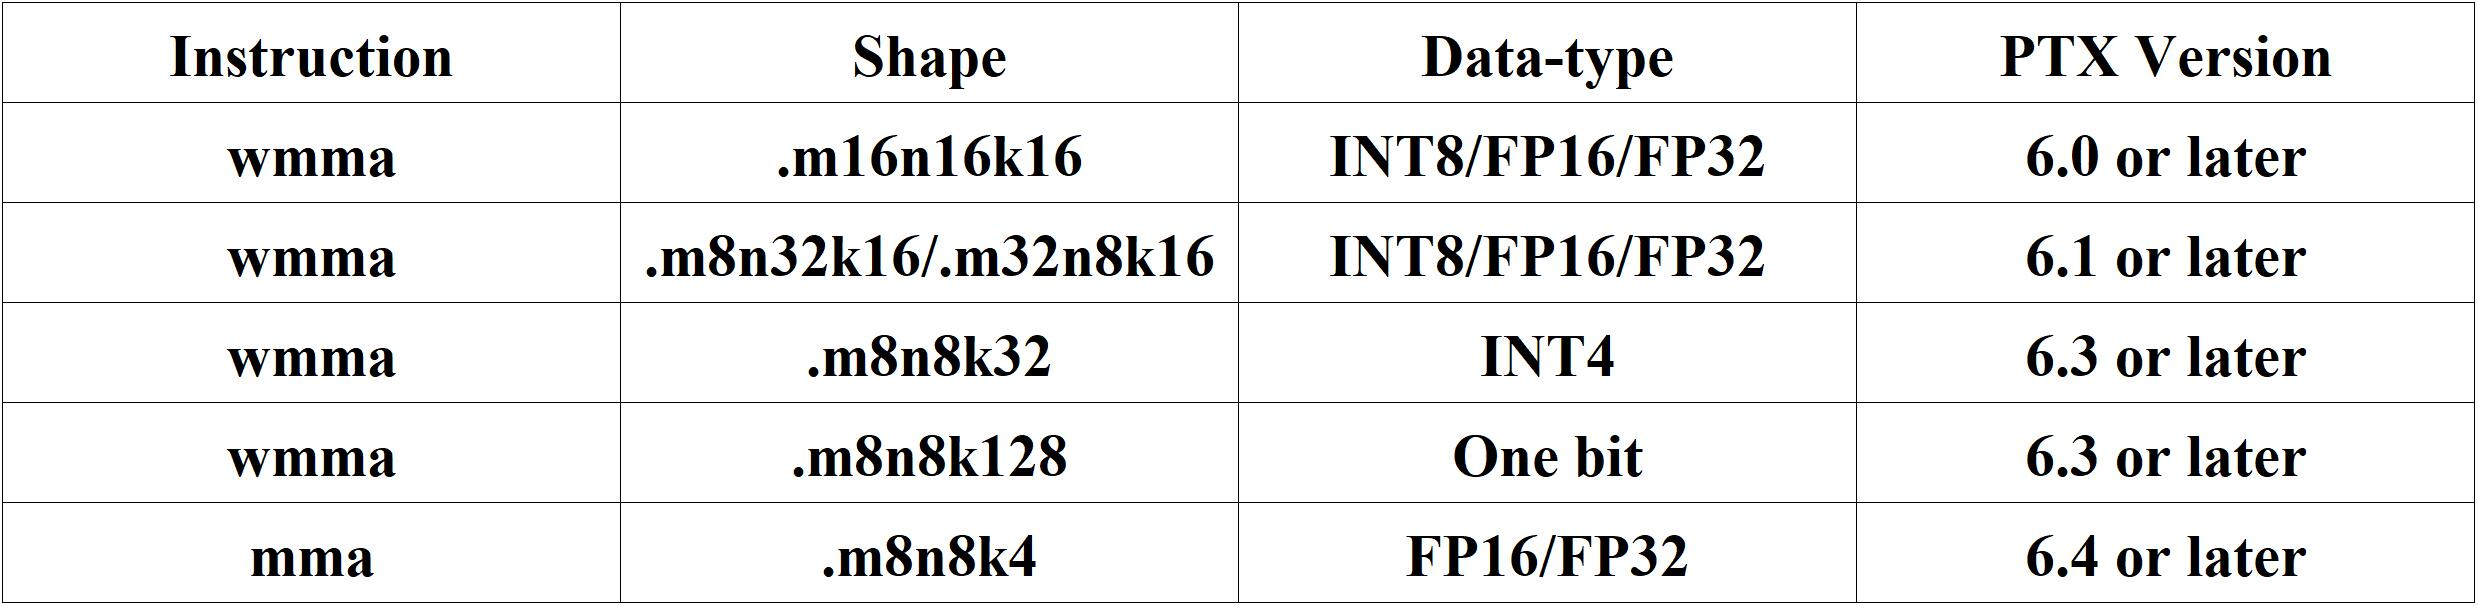
\includegraphics[width=15cm]{figures/WMMADOC.jpg}
	\renewcommand{\thefigure}{\arabic{section}-\arabic{figure} }
	\renewcommand{\figurename}{图}
	\caption{官方文档给出的wmma指令支持的分割尺寸\cite{PTX}}
	\addtocounter{figure}{-1}
	\renewcommand{\thefigure}{\arabic{section}-\arabic{figure} }
	\renewcommand{\figurename}{Figure}
	\caption{Matrix size supported in wmma instruction based on official documentation}
	\label{Fig.WMMADOC}
\end{figure}
\par 由于以上评估进行时GPU均为到达满载,故使用CUTLASS库评估了GPU满载时的矩阵乘加性能,如图 \ref{Fig-GEMM-CUTLASS}所示,可见在CUTLASS中以半精度浮点进行运算,开启张量核心(hgemm-wmma)后性能相比未开启张量核心(hgemm)提升了约3倍,与前文实验中相符;而其输入矩阵数据分布方式对性能有一定影响,总体来看,在半精度情况下(FP16),两矩阵均以行主元素存储的情况下性能较强(nt代表矩阵$ A $不进行转置,而矩阵$ B $进行转置,然而由于矩阵乘法运算的特征,矩阵$ B $转置表示其本身存储方式仍是行主元素存储;而tn则代表$ A $和$ B $都以列主元素存储),而两矩阵均以列主元素存储时性能较弱;然而在单精度情况下(FP32)时,四种运算性能差距不大,而总体运算性能也低于半精度时的运算性能,这也与在硬件层面张量核心以半精度为操作单元有关;而在双精度下(dgemm, double gemm)性能较差,这也与其硬件特征有关,即需要若干个低精度核心同步、合作计算高精度结果。值得注意的是,相对于CUTLASS 1.2版本,1.3版本新增了$ m=8,n=8,k=4 $的非跨线程束通用矩阵乘法(mma-gemm),这也是考虑到在数据规模较小时wmma会引发数量可观的同步、上下文切换,故新增了这一粒度的通用矩阵乘法。
\par 在实验平台中的NVIDIA Geforce RTX 2080TI搭载的TU102核心中有68个流多处理器单元\cite{2080TI},结合之前单个流处理器单元测试的性能,大约是60倍,这与硬件特征亦相符合,该结果将作为基准性能。从该试验得到的结果以及NVIDIA官方文档的资料,正如前文提到过,张量核心的计算最小粒度是$ 4\times 4 $然而在调度时仍然是以$ 16\times 16 $为单位,且两个线程束也被组织到一起进行执行;我们可以提出合理地猜想,在下一代架构的硬件中(安培架构),将会出现规模更大、跨越更多个线程束的矩阵乘加的指令集,以提高并行度进而进一步增加计算密集型任务的性能;当然,这样的指令也会在线程束之间的同步带来挑战。

\subsubsection{矩阵乘法运算}
\par 在新架构以矩阵乘加运算进行深度学习性能评估之前,大部分评估都采用单纯的矩阵乘法运算进行。自CUDA 6.0开始,NVIDIA推出了优化线性代数运算的cuBLAS库,而每次硬件架构更新,cuBLAS库均会针对新硬件做出改进、优化。最新的CUDA SDK 10.1则推出了cuBLASt轻量级库,在生成的应用程序大小方面做出了明显优化,性能方面则并无太多优化;由于本节旨在评估不使用张量核心的情况下,使用和不使用cuBLAS库的性能,而最新的cuBLAS库均针对张量核心进行优化,故本节中使用的cuBLAS库是基于CUDA SDK 8.0。本节将考察使用和不使用CUDA SDK 8.0中的cuBLAS库的情况下使用GPU进行矩阵乘法运算的性能。
\paragraph{实验结果}
\par 图 \ref{Fig.CUBLASPerf}显示了使用和不使用CUDA SDK 8.0中cuBLAS库进行矩阵乘法运算的性能。随着数据规模的增长,基于cuBLAS库的应用的单精度浮点矩阵乘法运算性能稳定在13TFlops左右;而不适用cuBLAS库的应用尽管不明显,其单精度浮点矩阵运算性能仍随着数据规模的增长而增长,最终稳定在0.13TFlops左右。实验中使用的数据集并未如上一节中测试张量核心时的数据,分为能否被8整除,而是全部随机。实验结果发现在张量核心以及相关指令尚未出现时,使用cuBLAS库时矩阵形状并不会对性能造成显著影响。
\begin{figure}
	\centering
	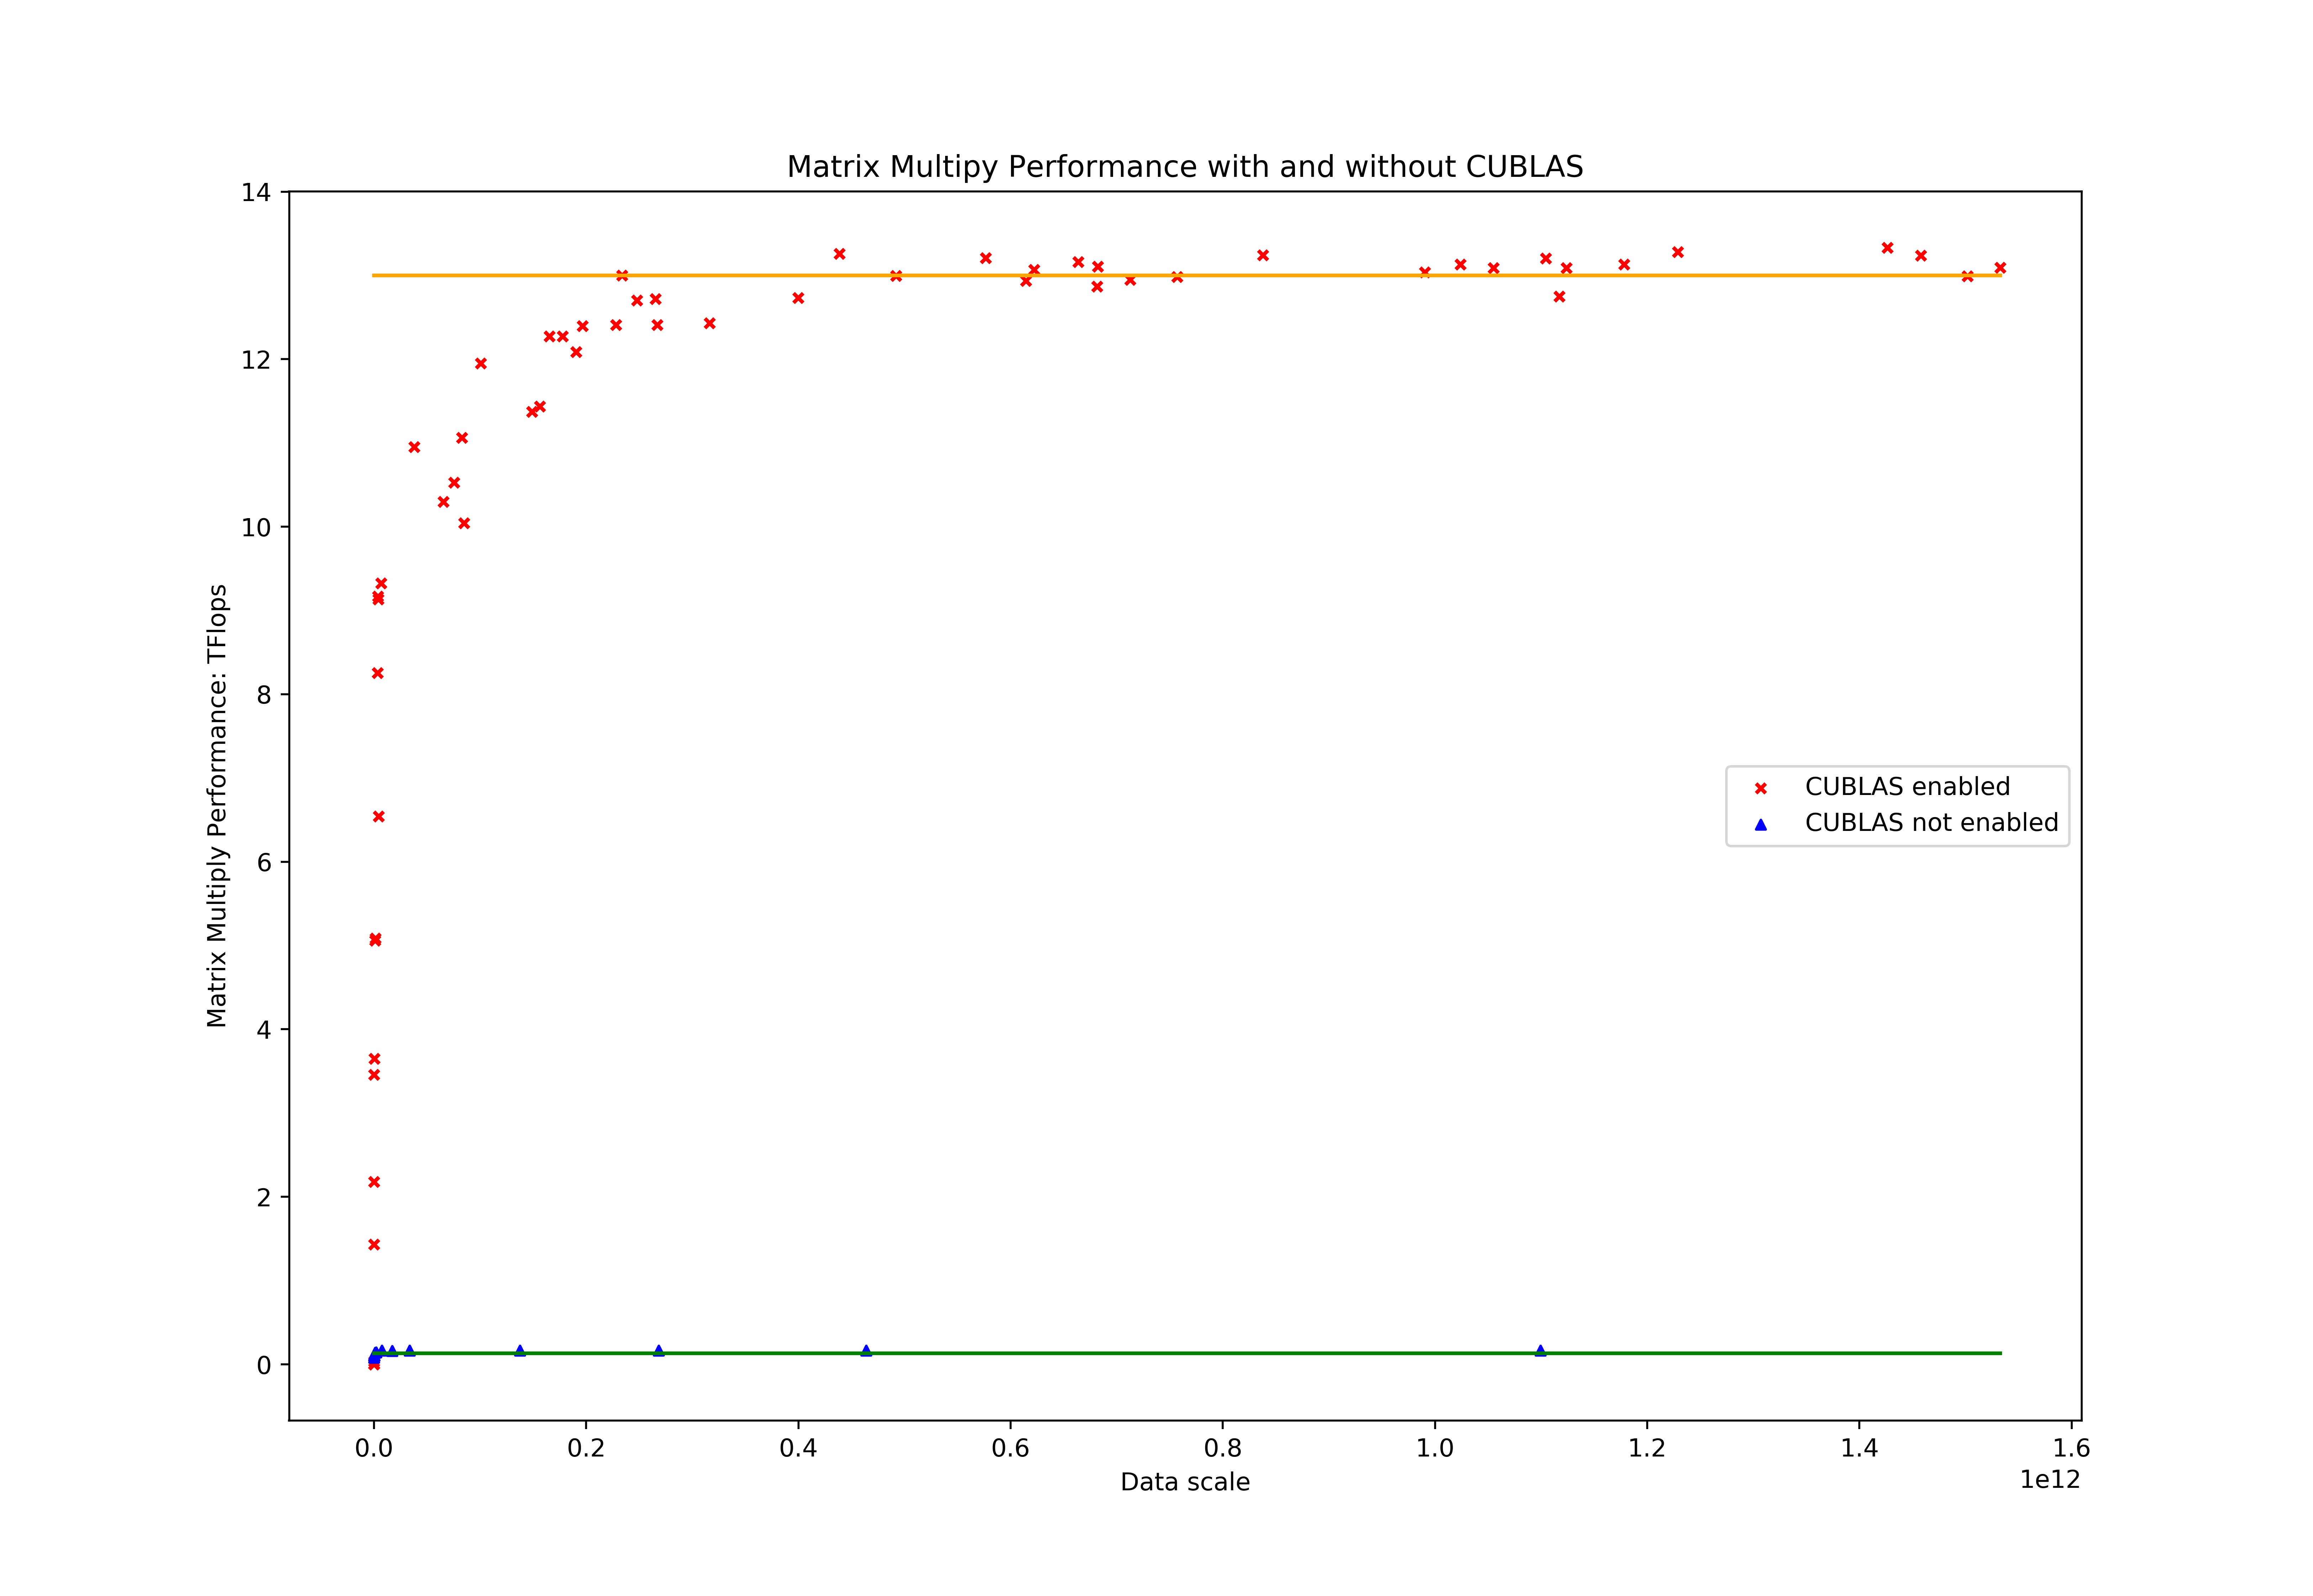
\includegraphics[width=15cm]{figures/CUBLASPerf.jpg}
	\renewcommand{\thefigure}{\arabic{section}-\arabic{figure} }
	\renewcommand{\figurename}{图}
	\caption{使用和不使用cuBLAS库时的矩阵乘法运算性能}
	\addtocounter{figure}{-1}
	\renewcommand{\thefigure}{\arabic{section}-\arabic{figure} }
	\renewcommand{\figurename}{Figure}
	\caption{Performance of Matrix Multiply with and without cuBLAS library}
	\label{Fig.CUBLASPerf}
\end{figure}
\paragraph{结果分析}
\par 需要注意的是,在实验中不使用cuBLAS库的矩阵乘法是基于GPU直接进行数值计算的,性能较差的同时支持的数据量也不够理想(因系统、硬件和驱动的原因,CUDA程序的一个内核在Windows 10操作系统下运行超过一定时间即会抛出超时异常,而不使用cuBLAS、采用直接计算的方法计算矩阵乘积速度较慢,导致大数据量下程序超时)。且由于内存分配模式的原因,在直接计算中,无法被32整除的维数需要被填充为32的倍数,在某些情况下会造成大量的内存浪费。故考虑到性能、程序健壮性等因素,在不支持张量核心的设备上进行矩阵乘法运算应尽可能使用cuBLAS库。

\subsubsection{卷积运算}
\par 在深度学习中,卷积作为提取特征、过滤图像噪声的一种方式,无疑是从业者最为熟悉、存在于最多应用中的计算。且在图像处理中,卷积运算也是非常重要的一环。计算卷积有若干方法,本节将使用NVIDIA官方发布的Benchmark样例评估这些不同方法在不同情况下的性能。当然,由于还存在解卷积运算,故精度也在本实验考虑范围之内,以满足不同任对队速度和精度的取舍。
\paragraph{实验结果}
\par 本节的实验涉及如下几种卷积计算方法:基于快速傅里叶变换的卷积;基于通用矩阵乘法的卷积和基于传统的直接计算的卷积(cudnn中将这一方法命名为Conv\_Direct),即卷积核滑动计算输出值。而这三种方法在CUDA的实现中也有差异,如表 \ref{table-CONV}所示。
\begin{table}
	\centering
	\renewcommand{\thetable}{\arabic{section}-\arabic{table} }
	\renewcommand{\tablename}{表}
	\caption{实验中的几种卷积计算方式}
	\addtocounter{table}{-1}
	\renewcommand{\thetable}{\arabic{section}-\arabic{table} }
	\renewcommand{\tablename}{Table}
	\caption{Methods to calculate convolution}
	\begin{tabular}{cc}
		\toprule
		卷积计算方式	&	描述\\
		\midrule
		基于快速傅里叶变换(FFT)的CUDA内建的卷积 & 使用CUDA提供的基于FFT的卷积库\\
		基于快速傅里叶变换(FFT)的自定义卷积 & 使用CUDA提供的FFT库实现卷积\\
		基于通用矩阵乘法(GEMM)的CUDA内建的卷积 & 使用CUDA提供的利用张量核心的API\\
		直接卷积(全局内存,Global Memory) & 直接计算每一个单元的值,基于全局内存\\
		直接卷积(纹理内存,Texture Memory) & 直接计算每一个单元的值,基于纹理内存\\
		\bottomrule
	\end{tabular} \label{table-CONV} 
\end{table}
\par 其中,访问纹理内存时使用传统的OpenCL/GL中的实现方式。因纹理内存的访存、缓存方式与一般存储系统不同,在测试时分为行卷积和列卷积。实验中卷积核步进、图像填充(padding)均不变,性能采用兆像素每秒(MPix/s)计算。
\begin{figure}
	\centering
	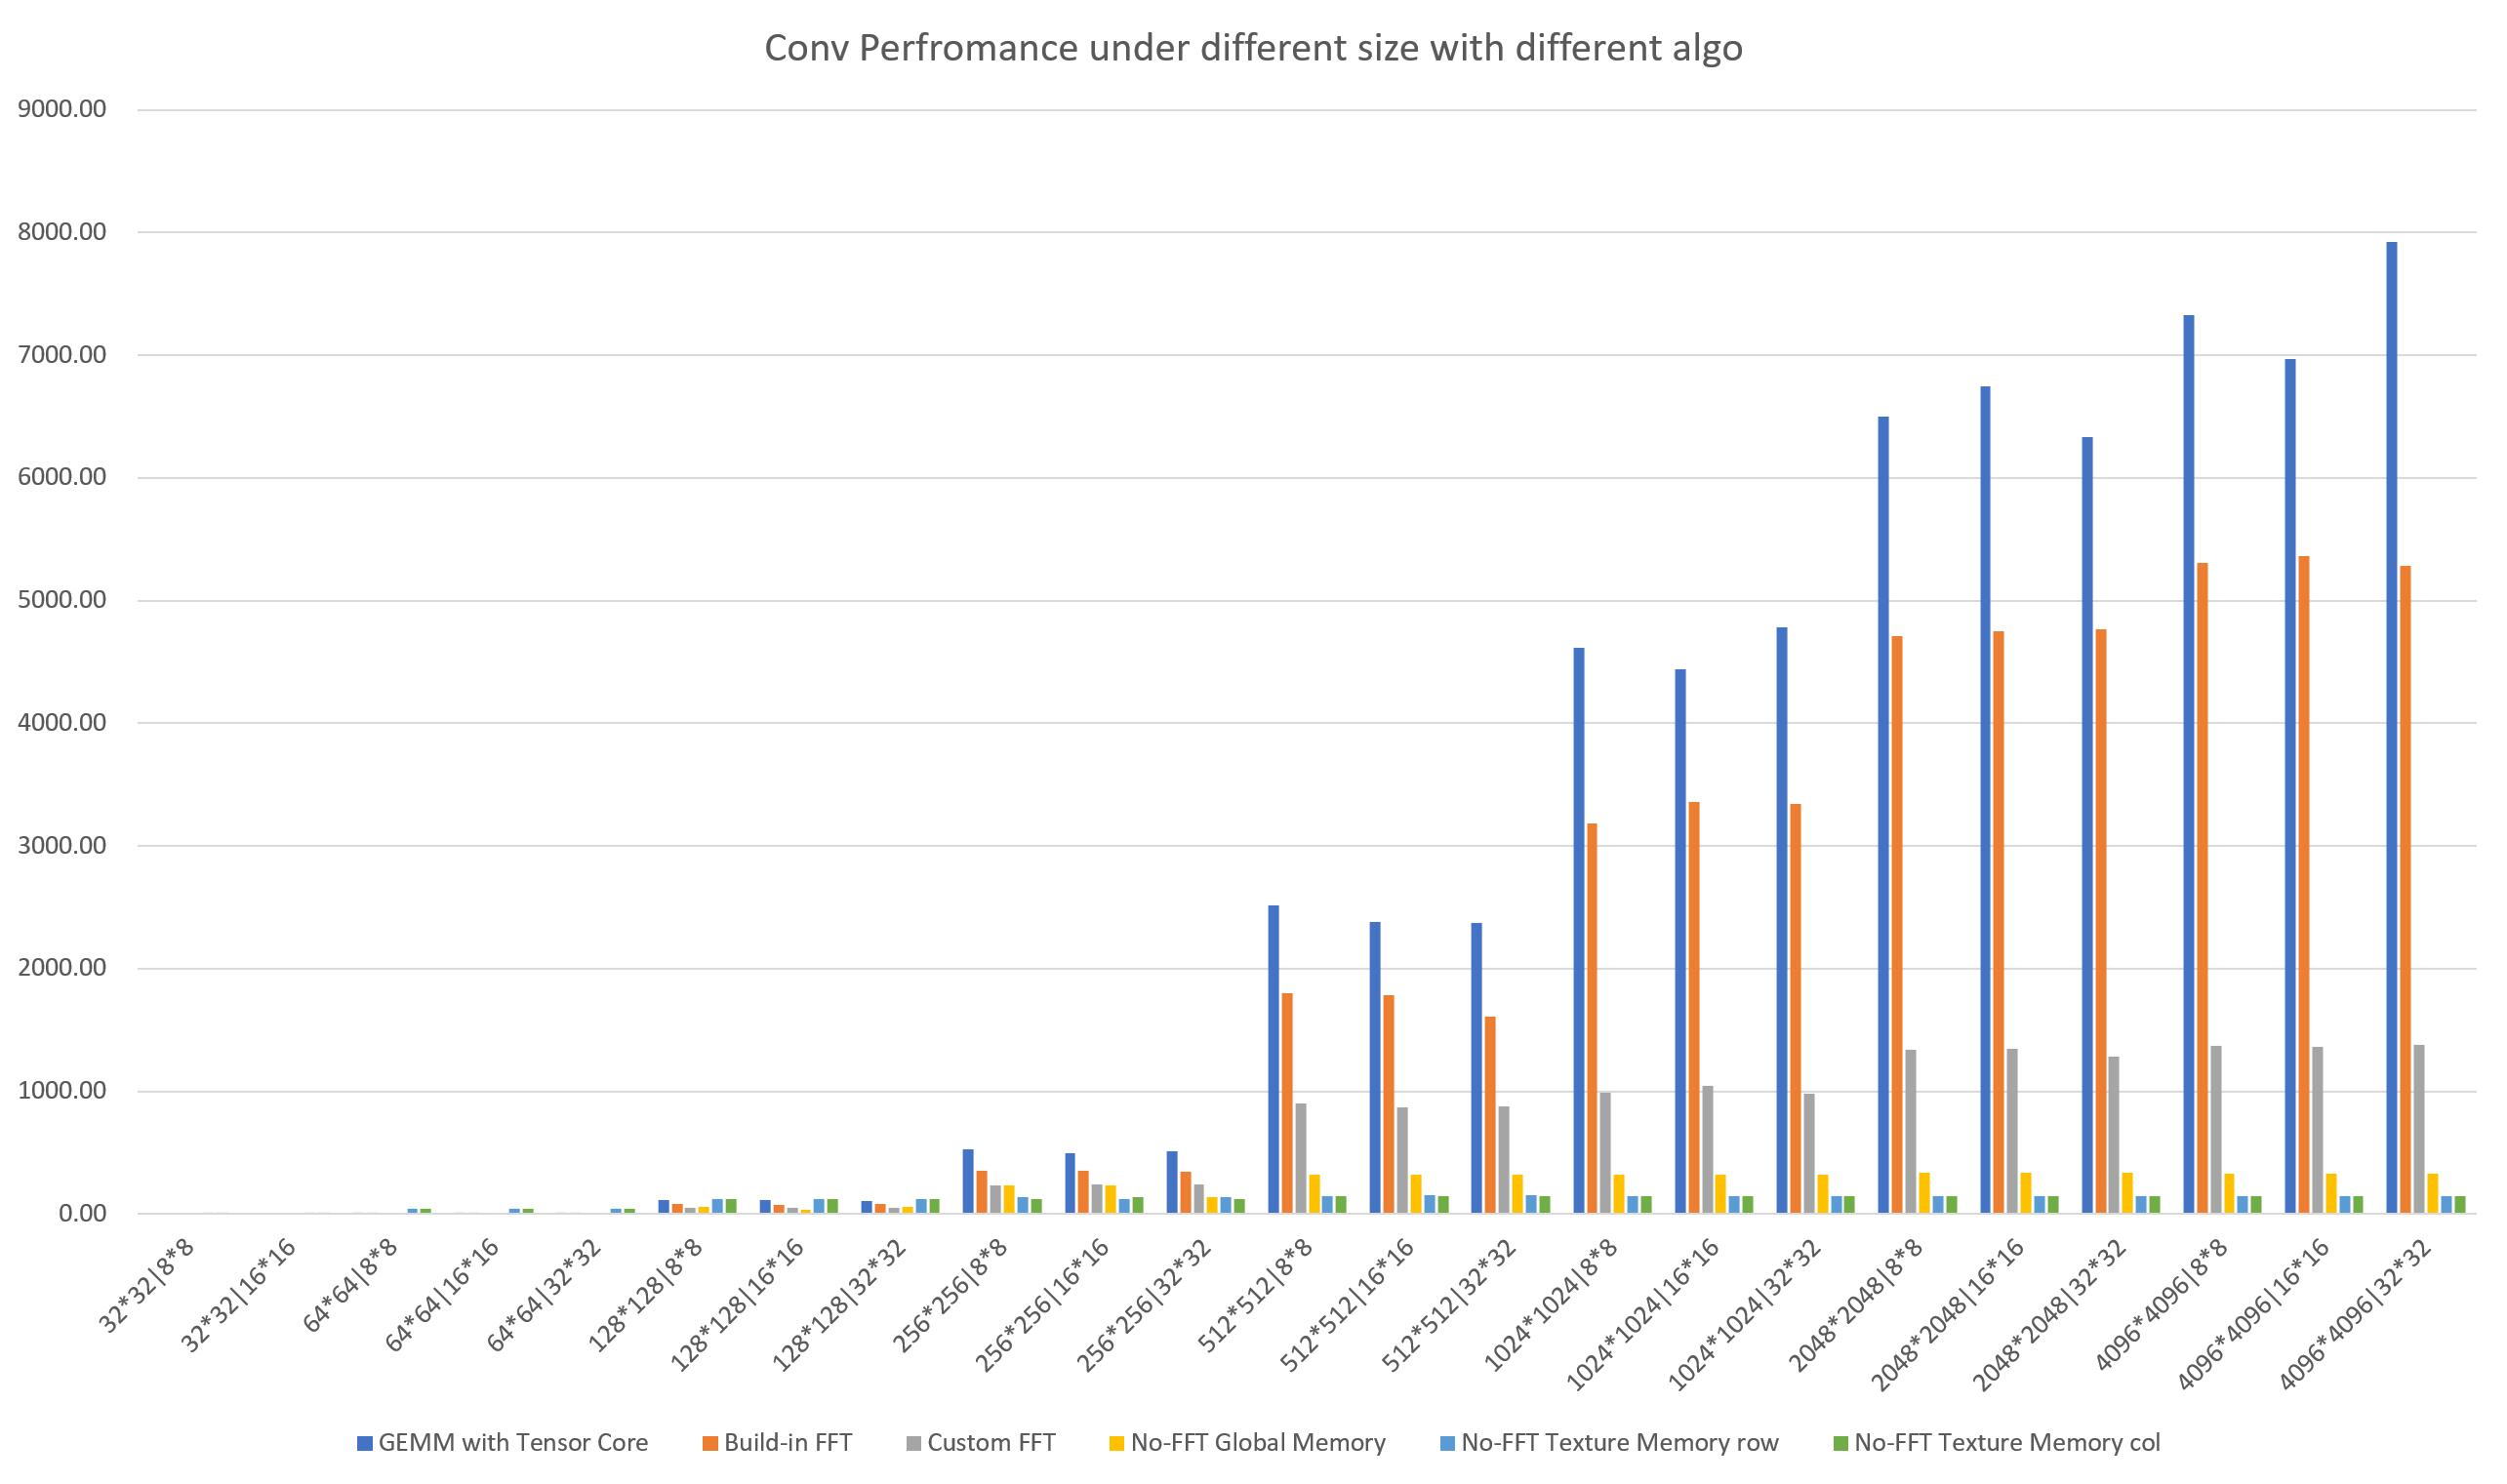
\includegraphics[width=15cm]{figures/CONVPerf.jpg}
	\renewcommand{\thefigure}{\arabic{section}-\arabic{figure} }
	\renewcommand{\figurename}{图}
	\caption{使用不同计算方法的卷积计算速度}
	\addtocounter{figure}{-1}
	\renewcommand{\thefigure}{\arabic{section}-\arabic{figure} }
	\renewcommand{\figurename}{Figure}
	\caption{Performance in speed of convolution based on different algorithm}
	\label{Fig.CONVPerf}
\end{figure}
\begin{figure}
	\centering
	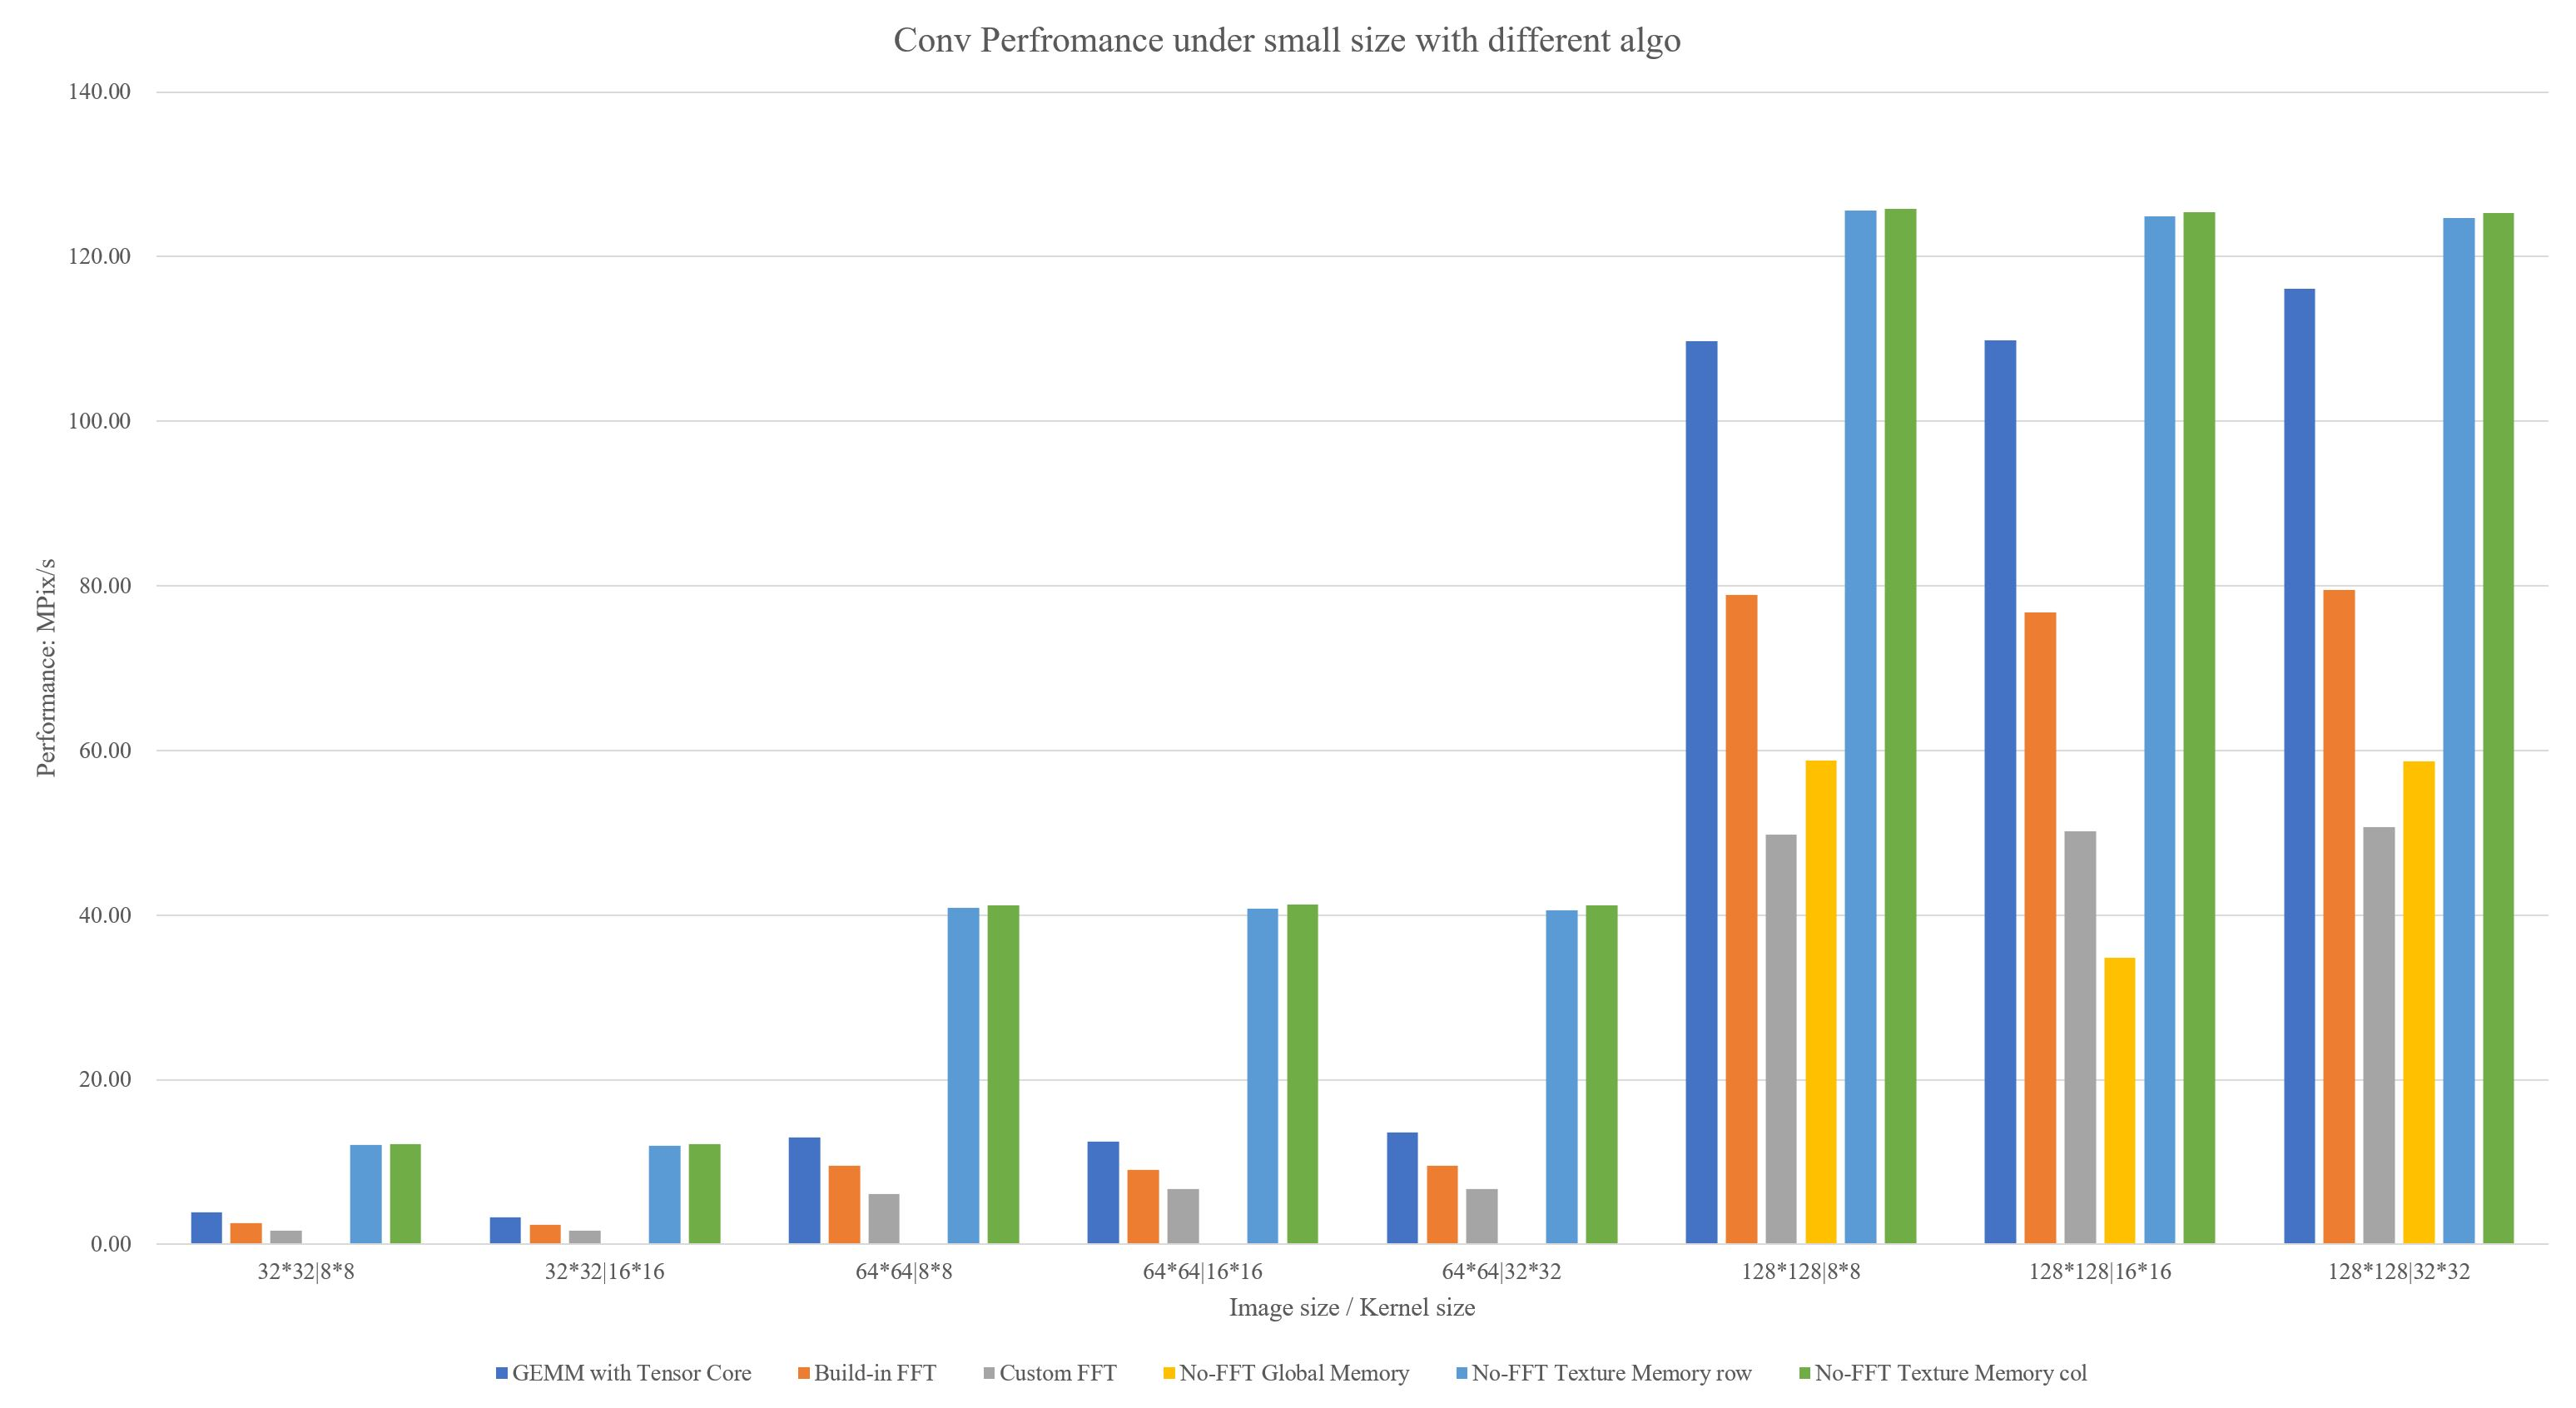
\includegraphics[width=15cm]{figures/CONVSubPerf.jpg}
	\renewcommand{\thefigure}{\arabic{section}-\arabic{figure} }
	\renewcommand{\figurename}{图}
	\caption{使用不同计算方法的卷积计算速度(小图像)}
	\addtocounter{figure}{-1}
	\renewcommand{\thefigure}{\arabic{section}-\arabic{figure} }
	\renewcommand{\figurename}{Figure}
	\caption{Performance in speed of convolution based on different algorithm(Small images)}
	\label{Fig.CONVSubPerf}
\end{figure}
\par 根据图 \ref{Fig.CONVPerf}中得到的关于卷积计算速度的实验结果可以得到如下结论,由于在图像尺寸较小是所有方法性能都较低,为了清晰比较图片尺寸较小时个方法的性能,图 \ref{Fig.CONVSubPerf}为图像尺寸小于$ 128\times 128 $时个方法的性能。首先,在输入图像尺寸较大时,基于通用矩阵乘法、使用张量核心的卷积计算方式和CUDA内建的基于快速傅里叶变换的卷积方式的性能优势相对于其他几种计算方式极为明显,而基于通用矩阵乘法的方法相比内建的基于快速傅里叶变换的方法性能高30\%-50\%、且随着图像尺寸的增加性能也增加,而卷积核尺寸对性能影响不大。在输入图像尺寸较小时,之前提到的两种方法性能急剧下降,而直接方法计算卷积性能较稳定;对于使用纹理内存的直接方法,行、列卷积差别不大。
\par 图 \ref{Fig.CONVPr}则是卷积计算精度的实验结果。首先,使用cuFFT库自行编写的基于快速傅里叶变换的卷积误差较大,达到$ 1\times 10^{-7} $级别,在许多实际应用中已经无法满足要求。而CUDA内建的基于快速傅里叶变换的卷积计算方式和基于通用矩阵乘法使用张量核心的卷积计算方式误差相近,都在$ 5\times 10^{-8} $级别;最后,直接方法计算卷积误差极低,基本为0,可以看作浮点数存储方式引发的误差。
\begin{figure}
	\centering
	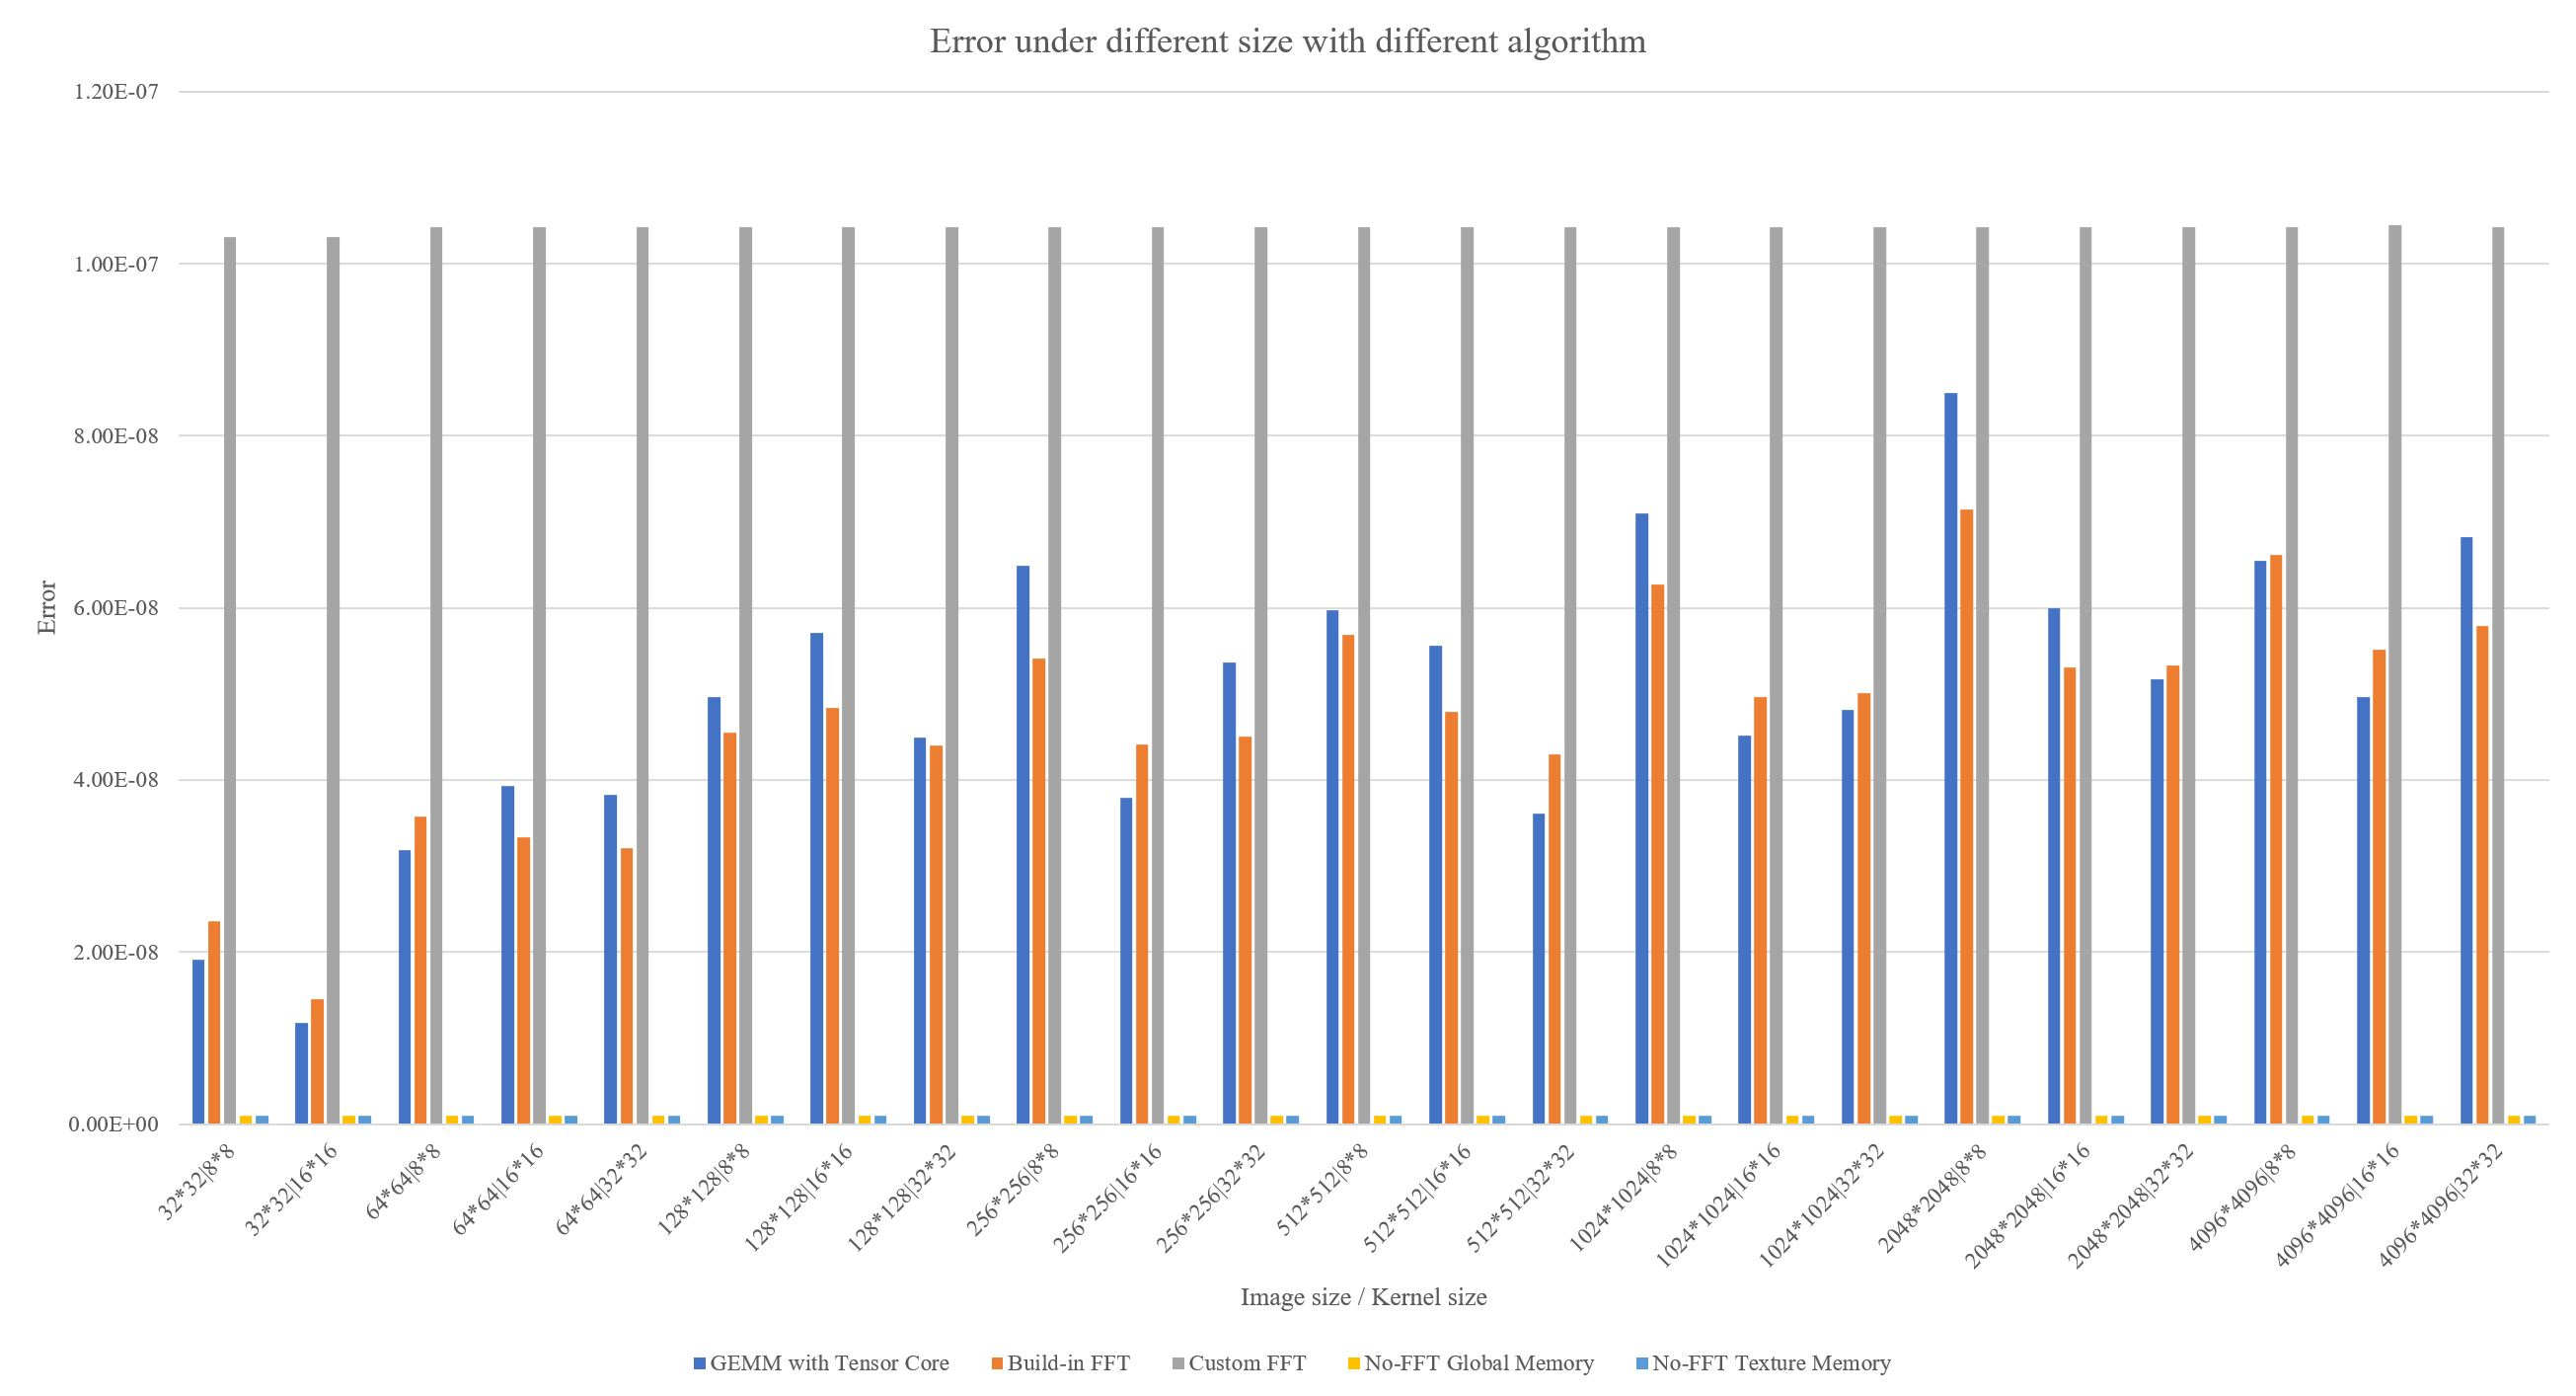
\includegraphics[width=15cm]{figures/CONVError.jpg}
	\renewcommand{\thefigure}{\arabic{section}-\arabic{figure} }
	\renewcommand{\figurename}{图}
	\caption{使用不同计算方法的卷积计算精度}
	\addtocounter{figure}{-1}
	\renewcommand{\thefigure}{\arabic{section}-\arabic{figure} }
	\renewcommand{\figurename}{Figure}
	\caption{Performance in accuracy of convolution based on different algorithm}
	\label{Fig.CONVPr}
\end{figure}
\paragraph{结果分析}
\par 在卷积计算速度方面,在图像尺寸较大的情况下,基于通用矩阵乘法的卷积计算方法和CUDA内建的基于快速傅里叶变换的卷积计算方法性能优势明显,且随着尺寸增大优势也愈大;在实际应用中可以根据SDK版本、硬件是否支持张量核心选择这两种计算方法。然而在图像尺寸较小时,直接方法计算卷积性能极大领先于其他方法,尤其是使用纹理内存进行优化后,性能达到基于通用矩阵乘法和快速傅里叶变换的计算方法的4-6倍。值得注意的是,在许多神经网络中,包括之后进行实验的卷积神经网络,其输入图像尺寸都是$ 10^2 $数量级,如$ 224\times 224, 128\times 128 $等,在该数量级上使用纹理内存优化的直接计算方法优势极大,本文也将基于这一结论对完整的卷积神经网络进行调整、优化。
\par 在卷积计算精度方面,基于通用矩阵乘法使用张量核心的方法基于FP16的精度进行计算;而基于快速傅里叶变换的方法在计算过程中需要将实数转为复数,再从复数转为实数,从而引入较大误差。而直接方法计算卷积由于直接对输出图像的每个单元进行计算,故误差极小可以忽略不计。在对精度要求极高的情况下,应选用直接方法计算卷积;值得注意的是,基于通用矩阵乘法和快速傅里叶变换的方法的精度已经达到$ 1\times 10^{-8} $级别,能够满足大部分情况的需求,故选择计算方法时仍需考虑输入图像大小。最后,基于快速傅里叶变换,但不使用内建API的方法不推荐使用,因在计算速度、计算精度方面,每种数据规格下都有更优选择。
\subsubsection{基于TensorRT的神经网络推理}
\par 上文提到了在机器学习应用中,对于模型的训练仅仅是第一步,在实际部署中,还有较大的优化空间。本实验中将使用TensorRT优化不同结构的网络,并搭配Jetson TX2套件进行运行。实验中的网络包括Inception、ResNet、mobileNet、vgg以及他们的变种、给定的训练好的模型。网络结构和相应特点以及实验目的在表 \ref{table-NETWORKS}中说明。
\begin{table}
	\centering
	\renewcommand{\thetable}{\arabic{section}-\arabic{table} }
	\renewcommand{\tablename}{表}
	\caption{网络推理实验中使用的网络及特点}
	\addtocounter{table}{-1}
	\renewcommand{\thetable}{\arabic{section}-\arabic{table} }
	\renewcommand{\tablename}{Table}
	\caption{Networks and their features used in inferencing}
	\begin{tabular}{cc}
		\toprule
		网络结构	&	描述\\
		\midrule
		Inception\_v1 & 网络深度、宽度较大,总体计算量较大\\
		ResNet\_v2 & 引入残差解决梯度、过拟合问题,网络可以更深\\
		Inveption\_v3 & 引入批归一化,使用$ 1\times n, n\times 1 $代替$ n\times n $卷积,卷积形状不同\\
		Inveption\_v4 & 使用残差优化的Inception\_v3\\
		Inveption\_resnet\_v2 & 结合Invenption与ResNet而生,与Inception\_v4较相似\\
		mobileNet\_v1 & 压缩网络规模,将标准卷积分解为深度卷积和逐点卷积\\
		vgg\_16 &  结构简化,但参数数量异常巨大,达1.38亿\\
		\bottomrule
	\end{tabular} \label{table-NETWORKS} 
\end{table}
\paragraph{实验结果}
\par 实验中首先使用原始的基于TensorFlow的模型在目标硬件(Jetson TX2)上以FP32的精度进行推理作为参照,然后使用经过TensorRT优化后的模型在目标硬件上以FP32和FP16的精度进行推理,旨在比较优化后的模型在推理方面的加速表现。图 \ref{Fig.INFER}为实验结果。
\begin{figure}
	\centering
	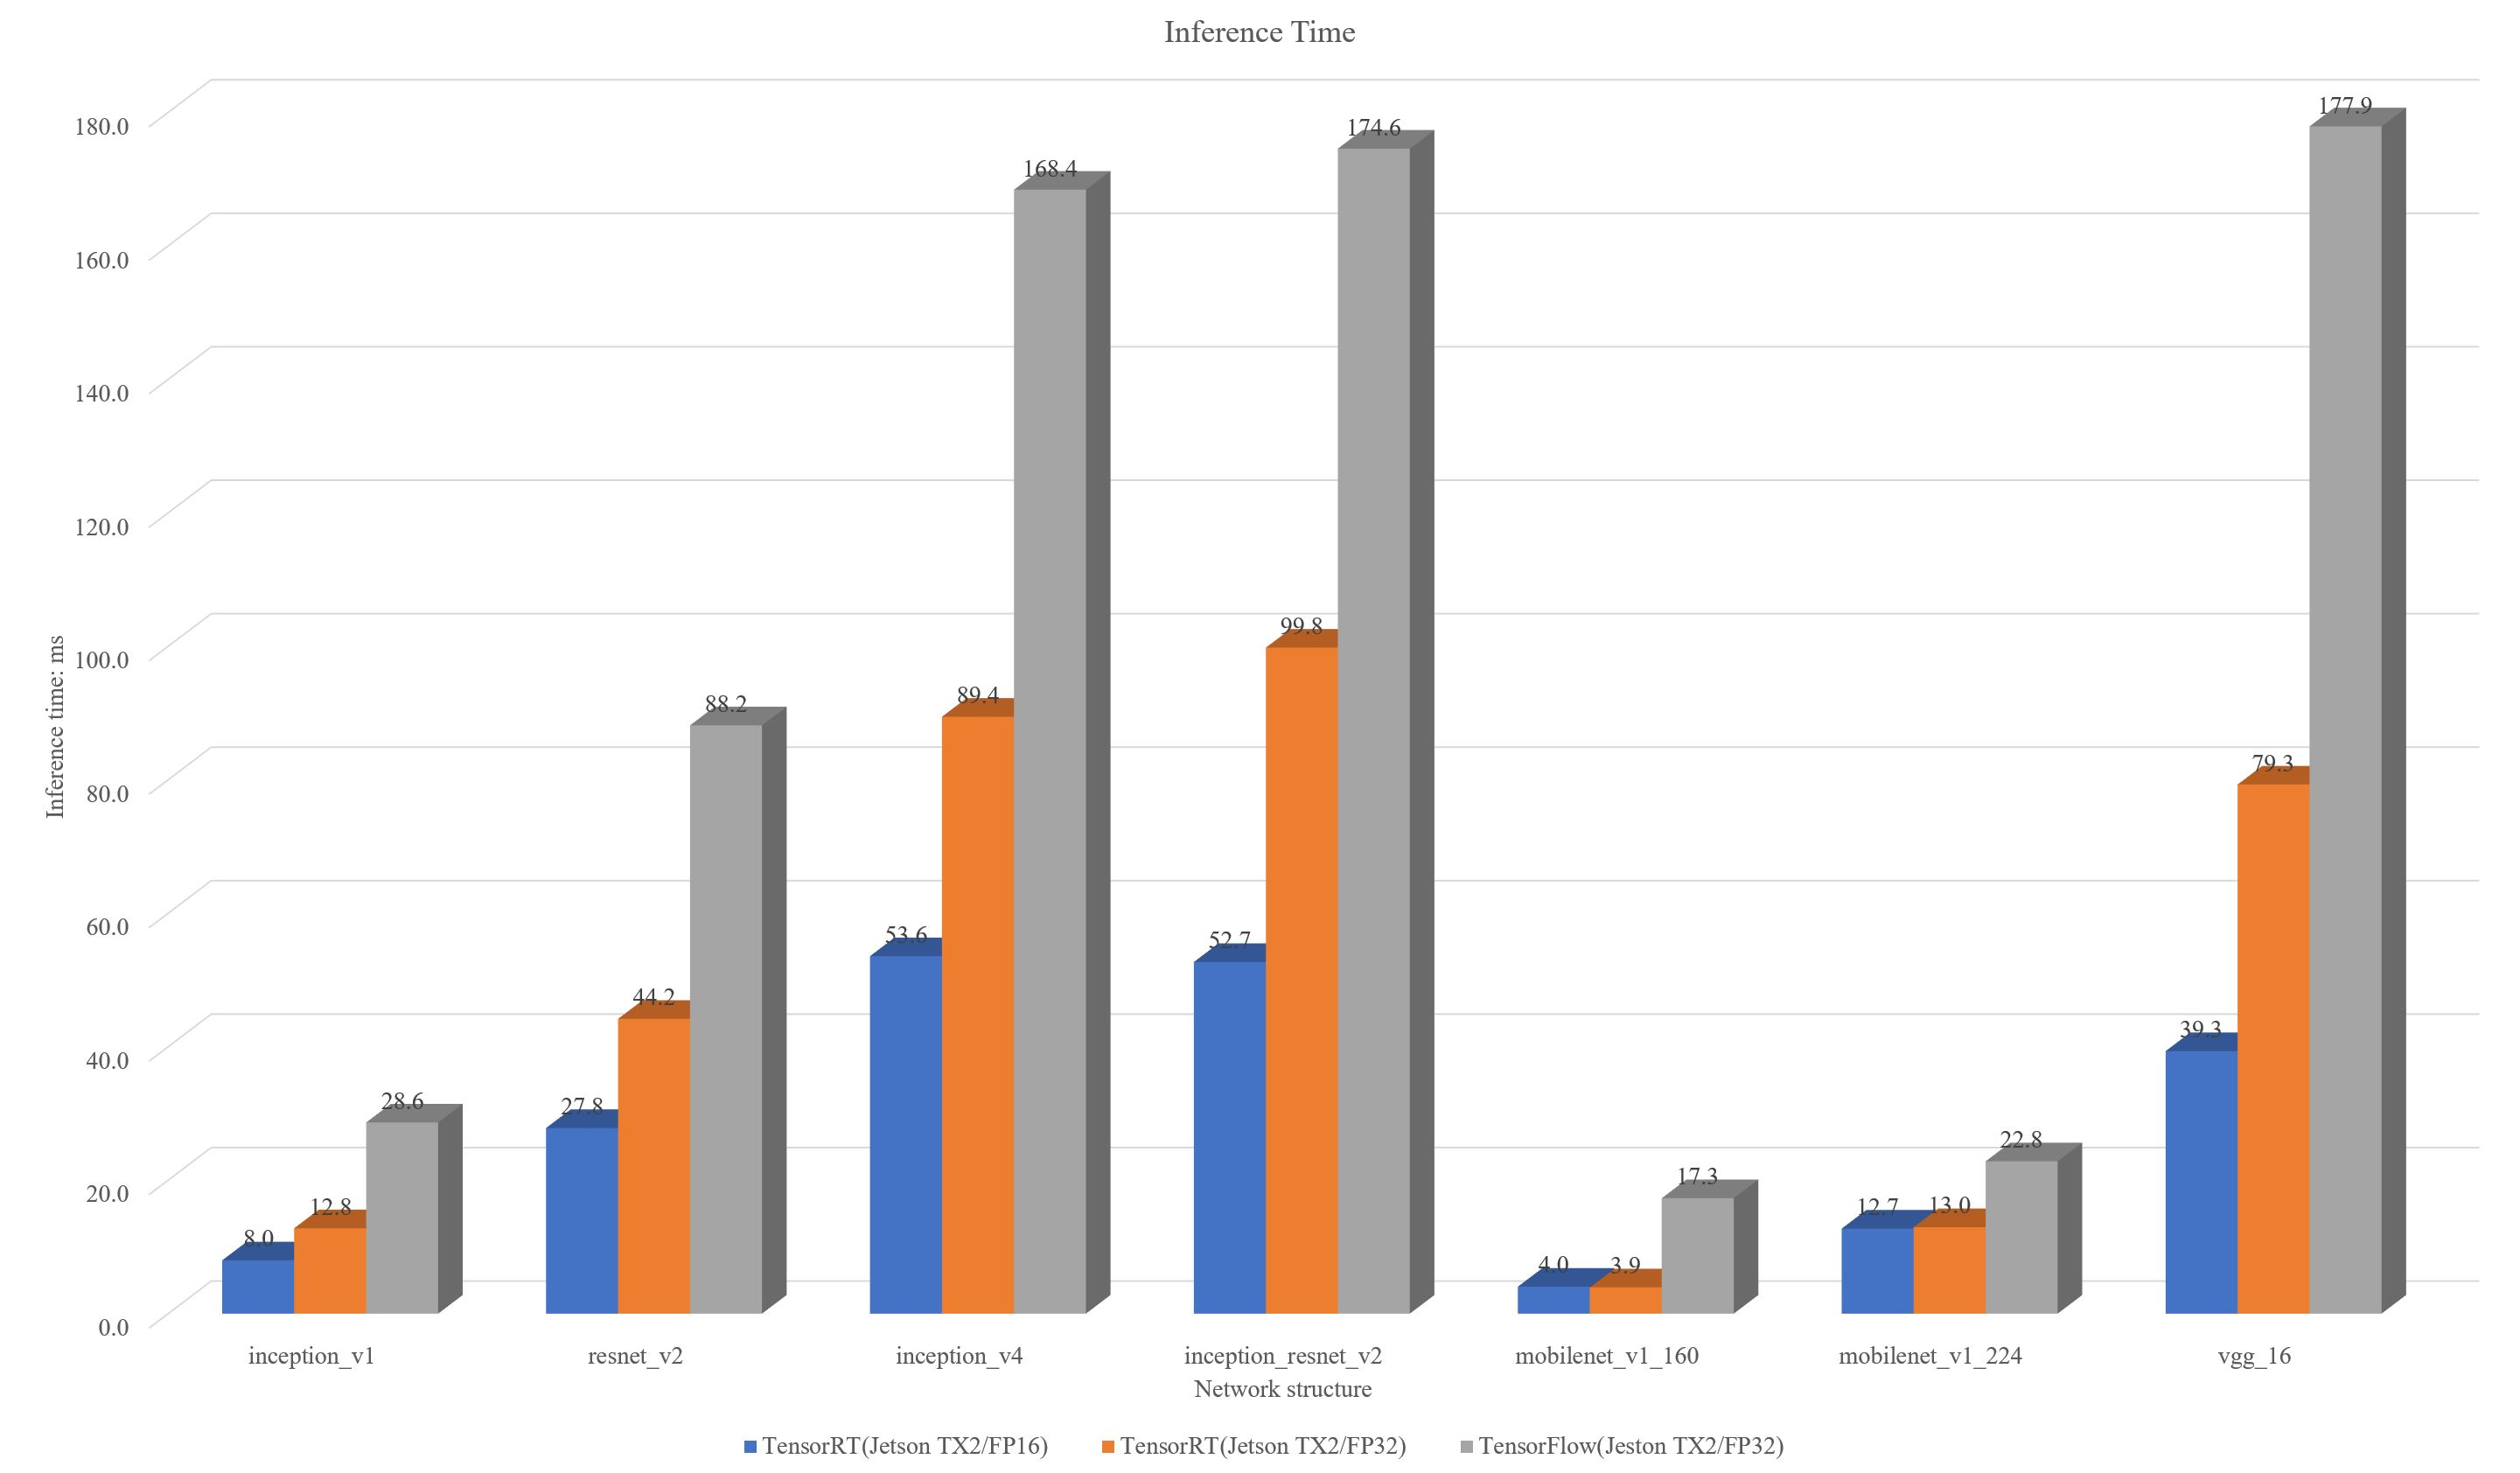
\includegraphics[width=15cm]{figures/TENSORRTRES.jpg}
	\renewcommand{\thefigure}{\arabic{section}-\arabic{figure} }
	\renewcommand{\figurename}{图}
	\caption{不同网络推理性能提升幅度}
	\addtocounter{figure}{-1}
	\renewcommand{\thefigure}{\arabic{section}-\arabic{figure} }
	\renewcommand{\figurename}{Figure}
	\caption{Increasing in inferencing of networks with different structure}
	\label{Fig.INFER}
\end{figure}
\par 在经过TensorRT对模型进行优化后,网络的推理性能或多或少有所提升,然而很明显不同结构的网络的总推力时间、提升幅度并不一致。其中提升最为明显的是vgg\_16网络。而面向嵌入式设备、移动设备的mobileNet推理时间相比其他网络而言非常短。而正如上文提到的,Inception\_v4与Inception\_Resnet\_v2较为相似,其推理时间以及提升幅度也较为相近。
\par 为了更完善了解网络结构、超参数等对于推理性能的影响,实验中还加入了一些网络的变体如不同层的ResNet、不同输入规模和分解方式mobileNet等,图 \ref{Fig.INFERSPEEDUP}显示了这些网络使用TensorRT优化后推理性能的加速比。
\begin{figure}
	\centering
	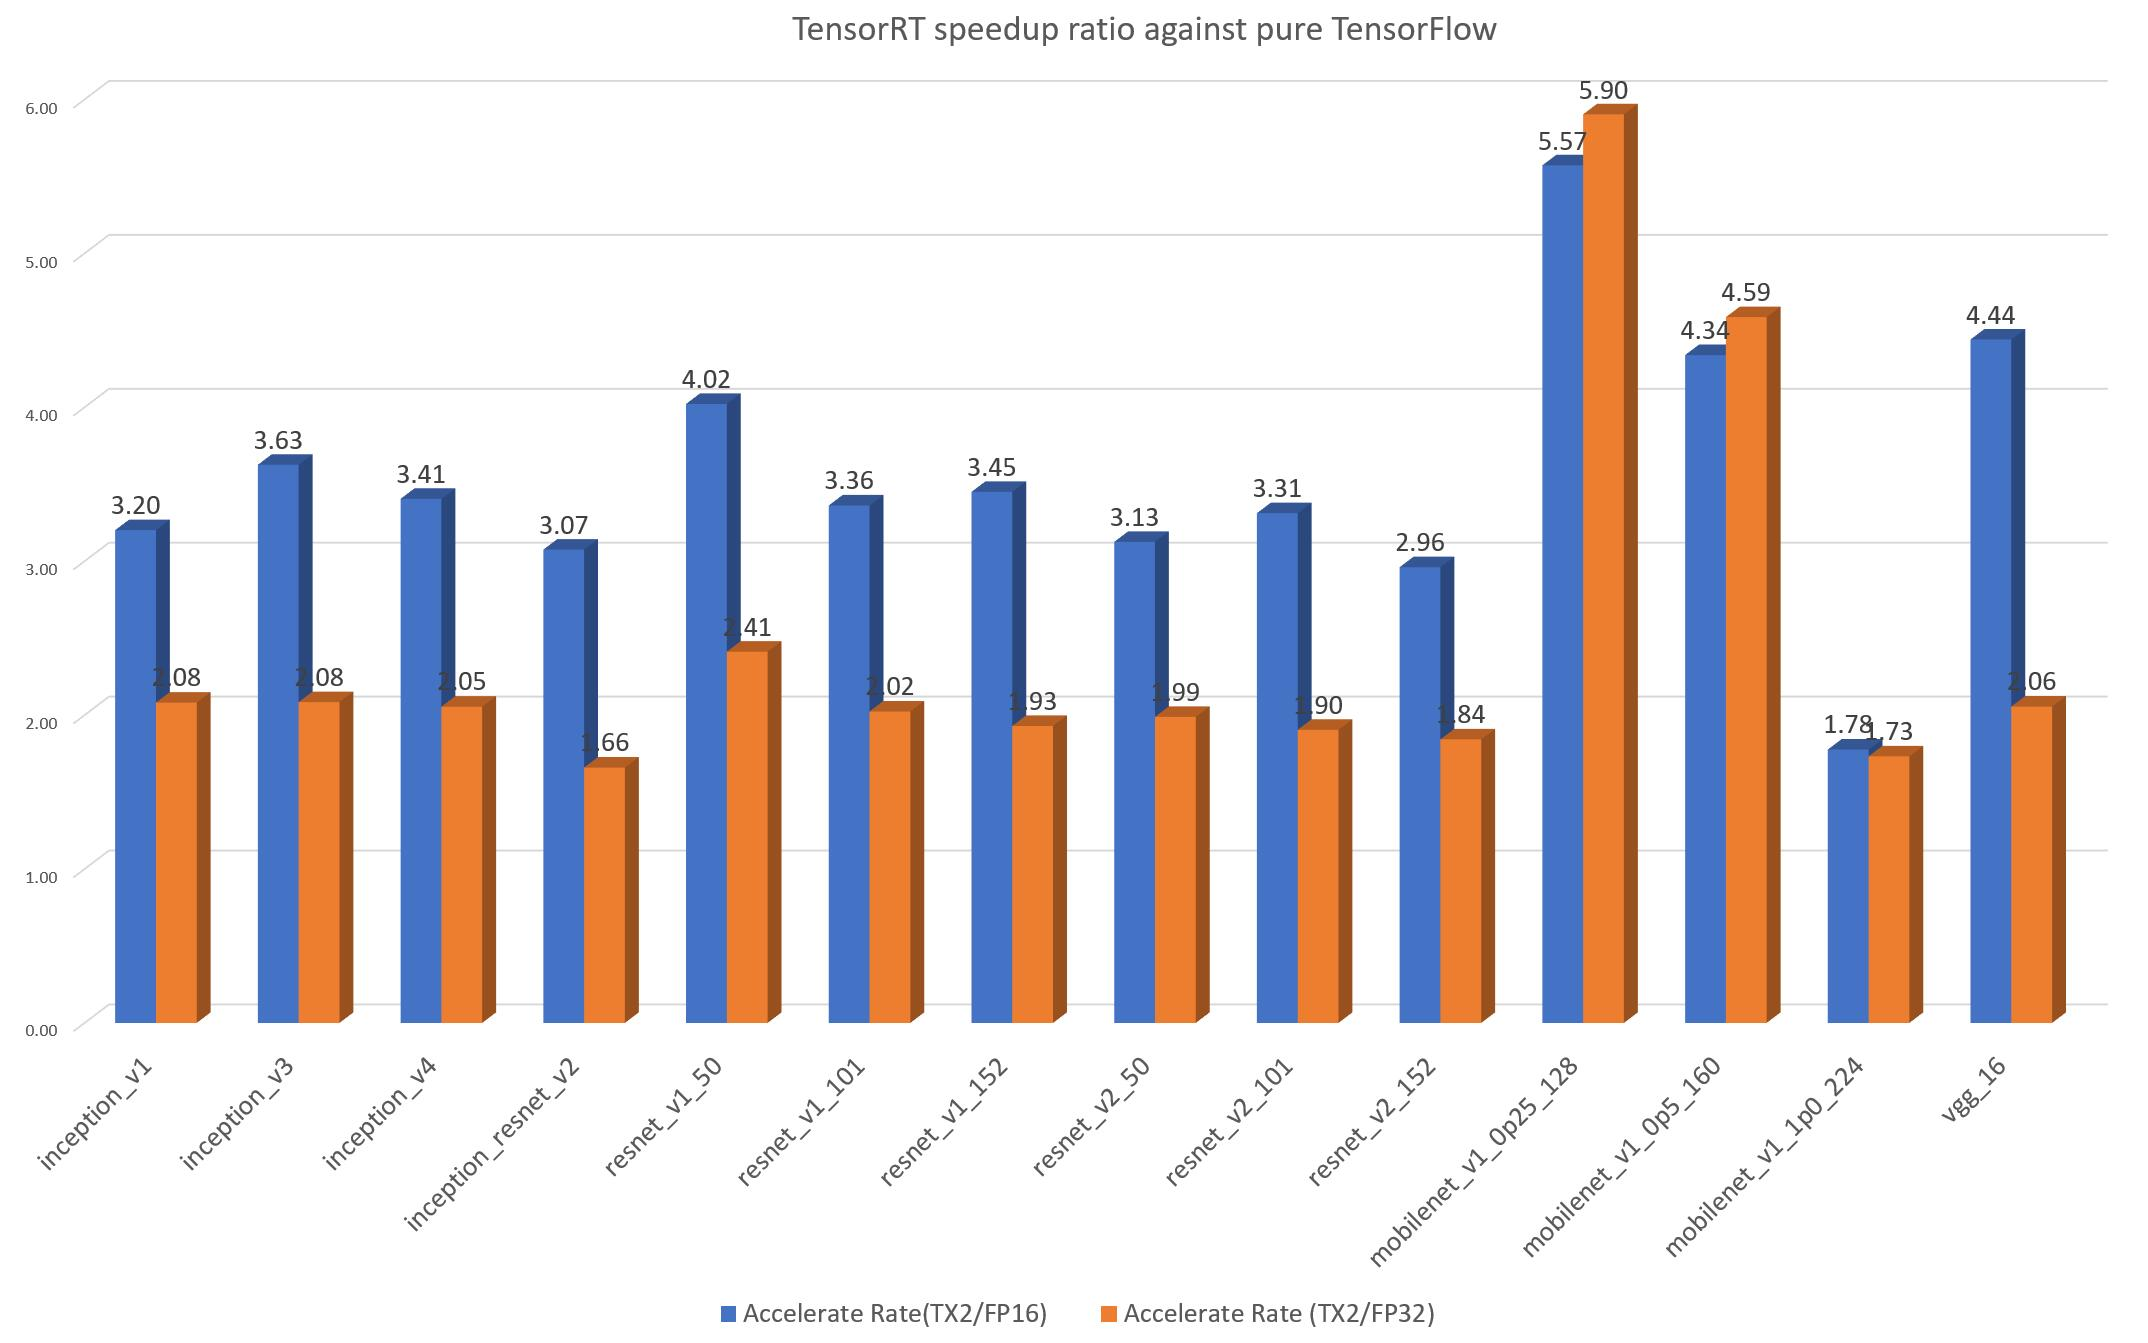
\includegraphics[width=15cm]{figures/TENSORRTRATIO.jpg}
	\renewcommand{\thefigure}{\arabic{section}-\arabic{figure} }
	\renewcommand{\figurename}{图}
	\caption{不同网络推理加速比}
	\addtocounter{figure}{-1}
	\renewcommand{\thefigure}{\arabic{section}-\arabic{figure} }
	\renewcommand{\figurename}{Figure}
	\caption{Speedup ratio in inferencing of networks with different structure}
	\label{Fig.INFERSPEEDUP}
\end{figure}
\par 在这些网络以及使用TensorRT优化后的加速比结果中,mobileNet的特征与其他网络差距较大,即FP16精度提升幅度反而比FP32精度提升幅度小。除此之外,与上文中的实验结果相符,vgg\_16网络的在FP16精度下提升幅度尤为明显。
\paragraph{结果分析}
\par 在实验使用的网络中,最具特色的无疑是mobileNet和vgg\_16两种。vgg\_16由于本身网络结构较简单,但是可训练参数的数量异常巨大,在使用原始模型推理时速度最慢,而在经过TensorRT优化后推理速度反超残差链接优化的Inception网络。可以看出结构单一、简单,但数量庞大的模型使用TensorRT优化后效果更佳,正如第二章中介绍的那样,TensorRT中最为重要的优化步骤即为将运算合并,对于结构单一但数量庞大的网络,这一优化的效果无疑是非常显著的。
\par 而面向嵌入式设备、移动端设备的mobileNet由于产品定位原因,其不使用TensorRT优化的推理速度已经非常理想,而测试集准确度与其余网络不相上下。然而,由TensorRT优化后的模型在FP16精度下的推理性能反而不如在FP32下的推理性能。其原因是mobileNet中将传统的三通道卷积(即长、宽、RGB)分解为针对长、宽的逐点卷积和针对RGB的$ 1\times 1\times Channel $的深度卷积,相应地在逐点和深度方向输出。而张量核心在进行矩阵乘加的加速时大量利用了FP16精度,即用精度换速度,运算时对输入矩阵的形状极为敏感,而$ 1\times 1 $的深度卷积与$ 4 \times 4 $的张量核心运算粒度相去甚远,故在FP16精度下的推理性能相较于FP32精度并无提升。值得注意的是,在mobileNet中随着输入图像尺寸的增加,使用TensorRT加速所取得的提升愈小,这也可以归咎于深度卷积的原因。
\subsection{基于CUDA源码的应用}
\par 本节将基于CUDA代码编写一系列实际的机器学习应用,以全方位评估实际使用中新架构硬件的加速性能以及相对于老架构硬件的加速幅度。本节选用如下几种算法:简单的卷积神经网络(CNN)和并行支持向量机算法(SVM)。在这些算法中包含了矩阵乘法、矩阵乘加、卷积以及浮点数值计算。评估中将采用NSight与nvprof分析运行情况。
\subsubsection{基于cuDNN的卷积神经网络(CNN)}
\par 由于本文的目的并不是提高特定一种机器学习应用或特定一种网络结构的性能,而是找到普适规律,故本节中的网络搭建参考了LeNet-5,并省略了池化层,仅保留输入/输出层、卷积层、全连接层。其原因是池化层中没有太多与本节需要评估的性能相关的运算,而输入/输出层时基本结构,卷积层中存在大量矩阵相关运算,全连接层由于其神经元大规模链接,是评估矩阵乘加的较好媒介。按照该网络结构,本节借助cuDNN搭建不同输入、连接、卷积尺寸的简化版卷积神经网络。实验数据集采用DeepBench中卷积神经网络对应的数据集。
\par 然而,与前文中单独评估卷积性能不同,在卷积神经网络中除卷积外还有另外的运算,故本节中对卷积神经网络的运算分为表 \ref{table-CONVSTEP}中所示的3个部分,旨在更准确、完善地评估新架构硬件在一个完整的卷积神经网络运算中所能带来的提升。表 \ref{table-FWDALGO}和表 \ref{table-BWDALGO}列出了cudnnConvolution中的前向传播和反向传播算法根据表中描述的特征,在试验前猜测前向传播部分的性能能通过张量核心获得一定提升,而另外两个部分的性能提升幅度不会太明显,即基本持平。
\begin{table}
	\centering
	\renewcommand{\thetable}{\arabic{section}-\arabic{table} }
	\renewcommand{\tablename}{表}
	\caption{卷积神经网络中的3个计算部分}
	\addtocounter{table}{-1}
	\renewcommand{\thetable}{\arabic{section}-\arabic{table} }
	\renewcommand{\tablename}{Table}
	\caption{3 parts in Convulutional Neural Network}
	\begin{tabular}{ccc}
		\toprule
		过程 & cuDNN::cudnnConvolution-	&	描述\\
		\midrule
		前向传播 & Forward() & 包含大量卷积、混合矩阵运算 \\
		反向传播更新卷积核权重 & BackwardFilter() & 包含大量梯度、浮点数值计算,设计卷积运算\\
		反向传播更新连接权重 & BackwardData() & 包含大量梯度、浮点数值计算\\
		\bottomrule
	\end{tabular} \label{table-CONVSTEP} 
\end{table}
\begin{table}
	\centering
	\renewcommand{\thetable}{\arabic{section}-\arabic{table} }
	\renewcommand{\tablename}{表}
	\caption{cudnnConvolution中前向传播算法}
	\addtocounter{table}{-1}
	\renewcommand{\thetable}{\arabic{section}-\arabic{table} }
	\renewcommand{\tablename}{Table}
	\caption{Forward algorithm in cudnn}
	\begin{tabular}{cc}
		\toprule
		算法 & 描述\\
		\midrule
		IMPLICIT\_GEMM & 隐式GEMM,即不显式构造容纳张量数据的矩阵\\
		IMPLICIT\_PRECOMP\_GEMM & 预处理的隐式GEMM\\
		GEMM & 显式GEMM,即显式构造容纳张量数据的矩阵\\
		DIRECT & 直接滑块计算方法\\
		FFT & 快速傅里叶变换\\
		FFT\_TILING & 分割输入的快速傅里叶变换\\
		WINOGRAD & 通过矩阵变换将部分乘法操作替换为加法操作\\
		\bottomrule
	\end{tabular} \label{table-FWDALGO} 
\end{table}
\begin{table}
	\centering
	\renewcommand{\thetable}{\arabic{section}-\arabic{table} }
	\renewcommand{\tablename}{表}
	\caption{cudnnConvolution中反向传播算法}
	\addtocounter{table}{-1}
	\renewcommand{\thetable}{\arabic{section}-\arabic{table} }
	\renewcommand{\tablename}{Table}
	\caption{Backward algorithm in cudnn}
	\begin{tabular}{cc}
		\toprule
		算法 & 描述\\
		\midrule
		FFT & 快速傅里叶变换\\
		FFT\_TILING & 分割输入的快速傅里叶变换\\
		WINOGRAD & 通过矩阵变换将部分乘法操作替换为加法操作\\
		\bottomrule
	\end{tabular} \label{table-BWDALGO} 
\end{table}
\paragraph{实验结果}
\par 实验结果如图 \ref{Fig.CNNPerf-1}和图 \ref{Fig.CNNPerf-2}所示。该实验结果在一定程度上应证了猜想:张量核心能够为网络的前向传播部分带来大约20\%-40\%的提升,稍低于前文中评估的基于矩阵乘加使用张量核心进行的卷积计算相对于内建快速傅里叶变换的卷积计算的性能提升幅度,因前向传播并非纯粹的卷积计算,该差距在合理范围内;然而其余部分的性能开启张量核心后均有一定程度的落后。
\begin{figure}
	\centering
	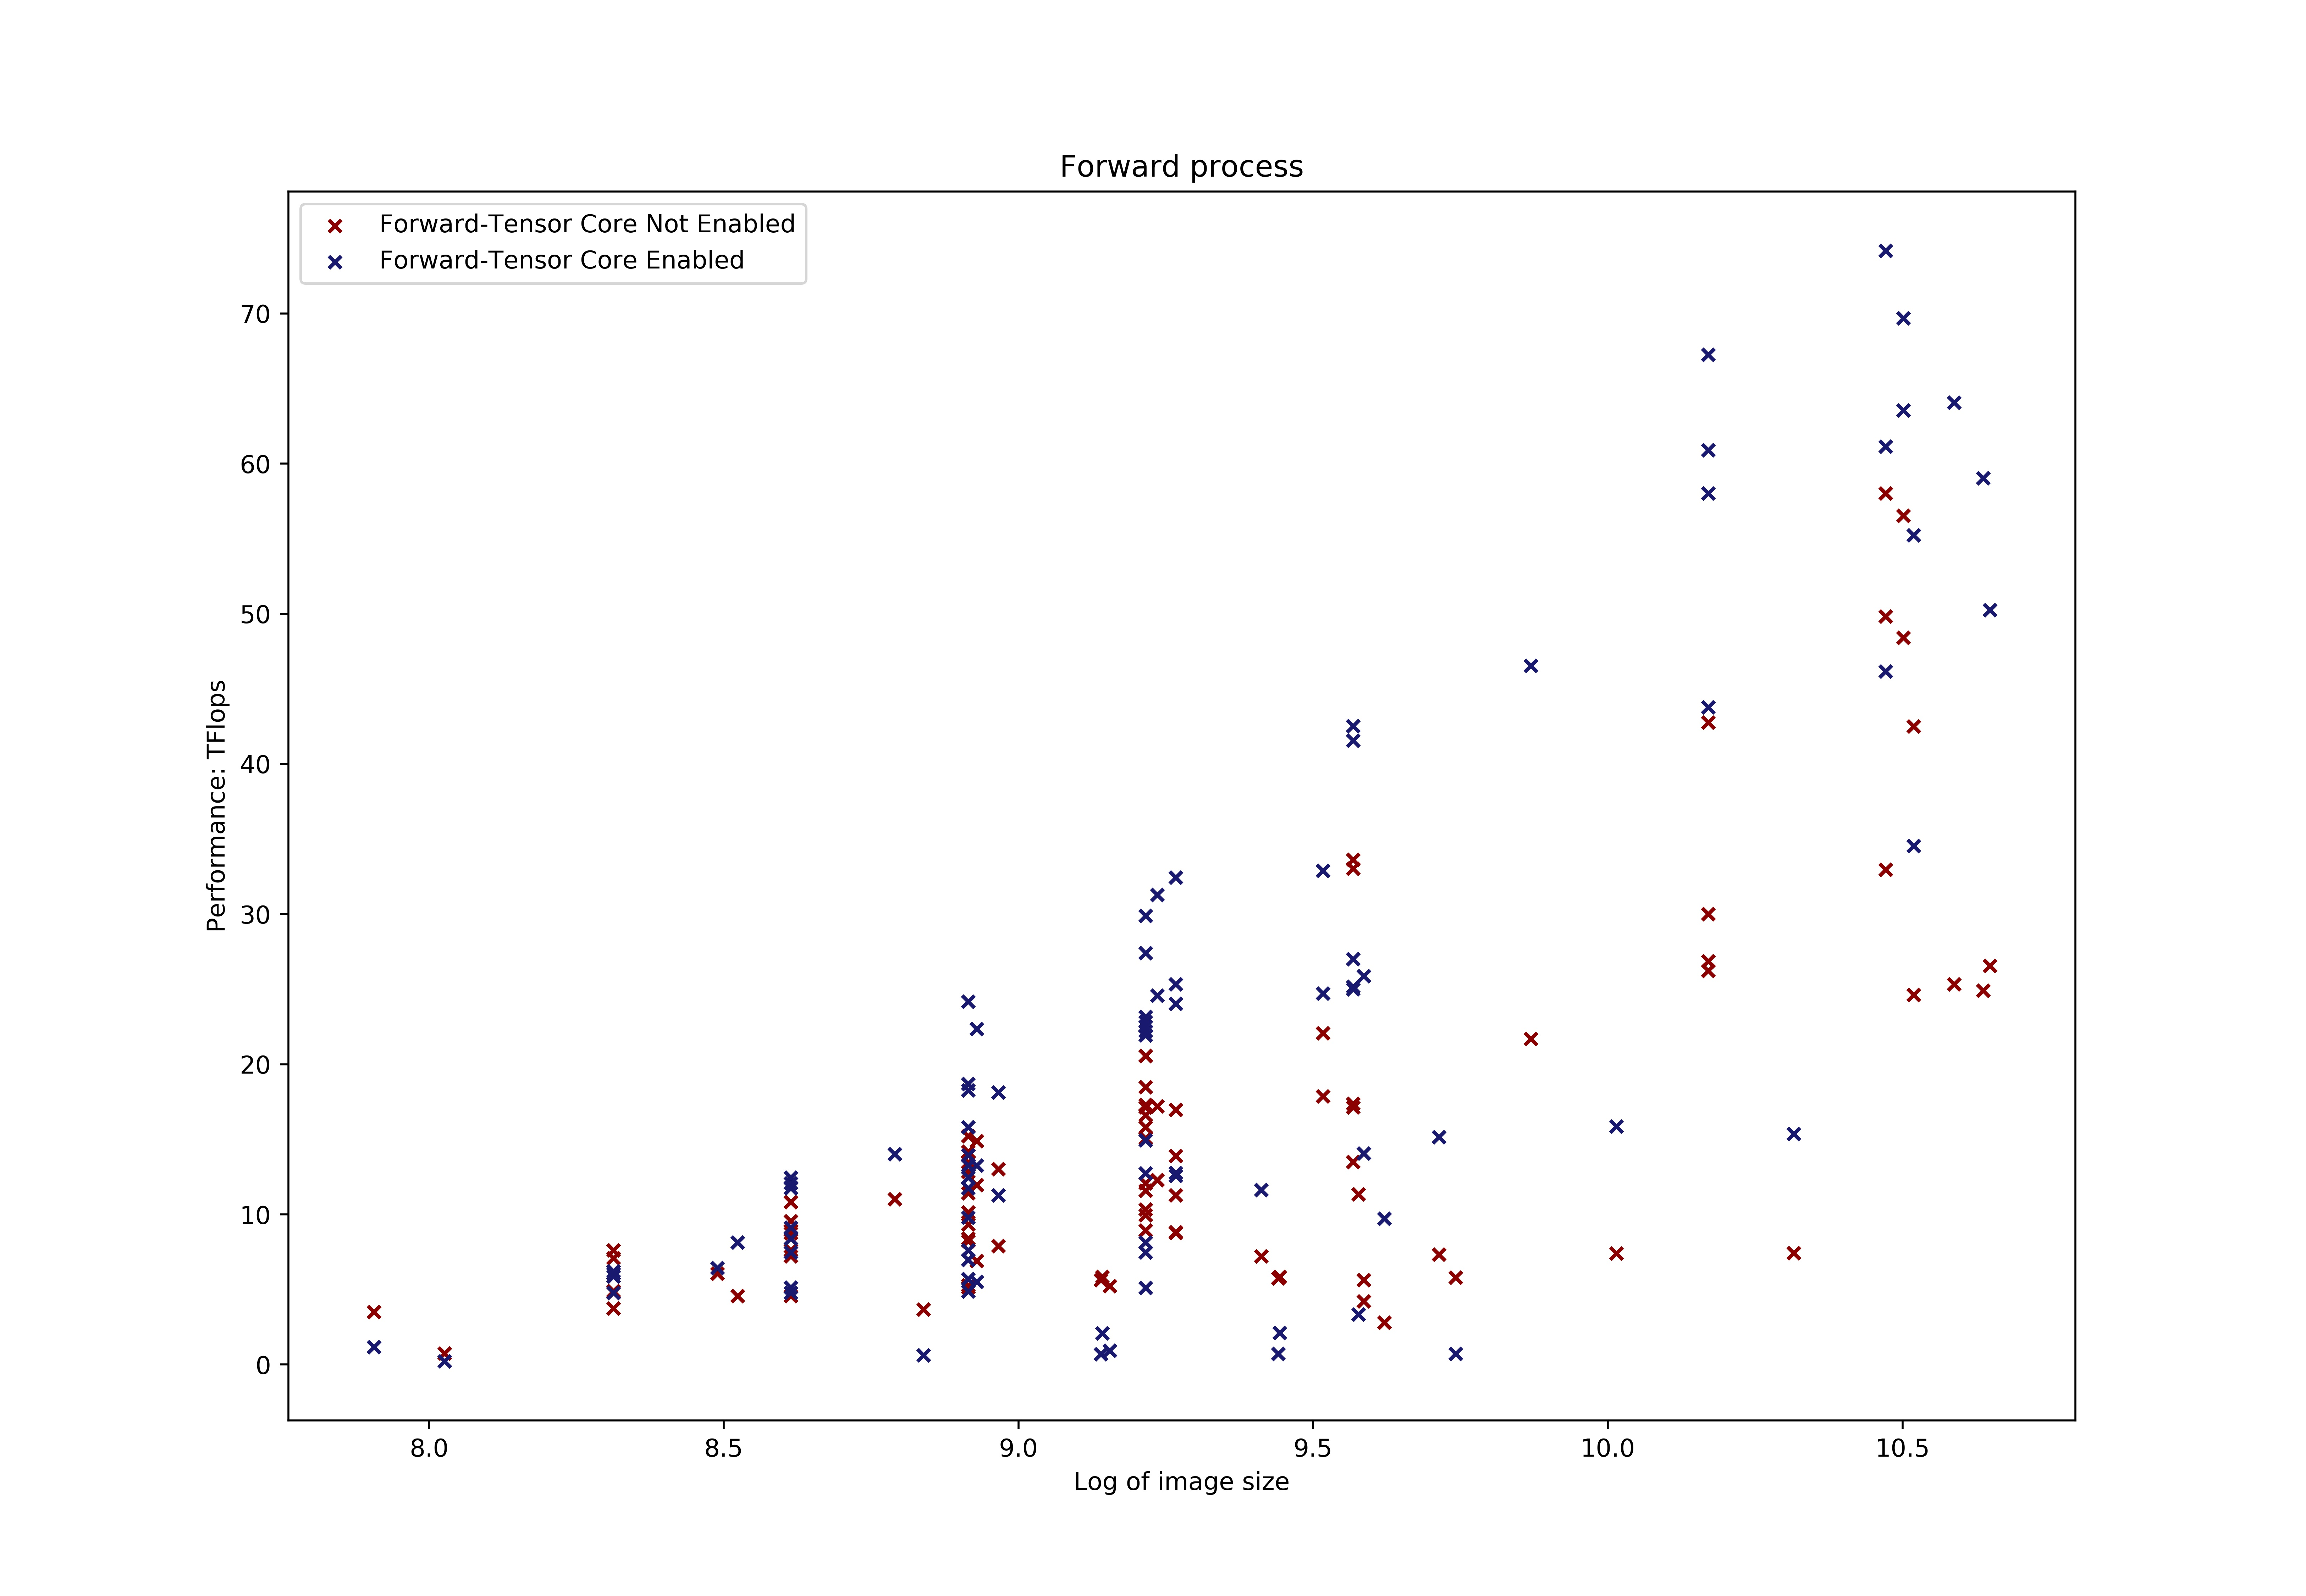
\includegraphics[width=15cm]{figures/CNN-HALF-FWD.jpg}\\
	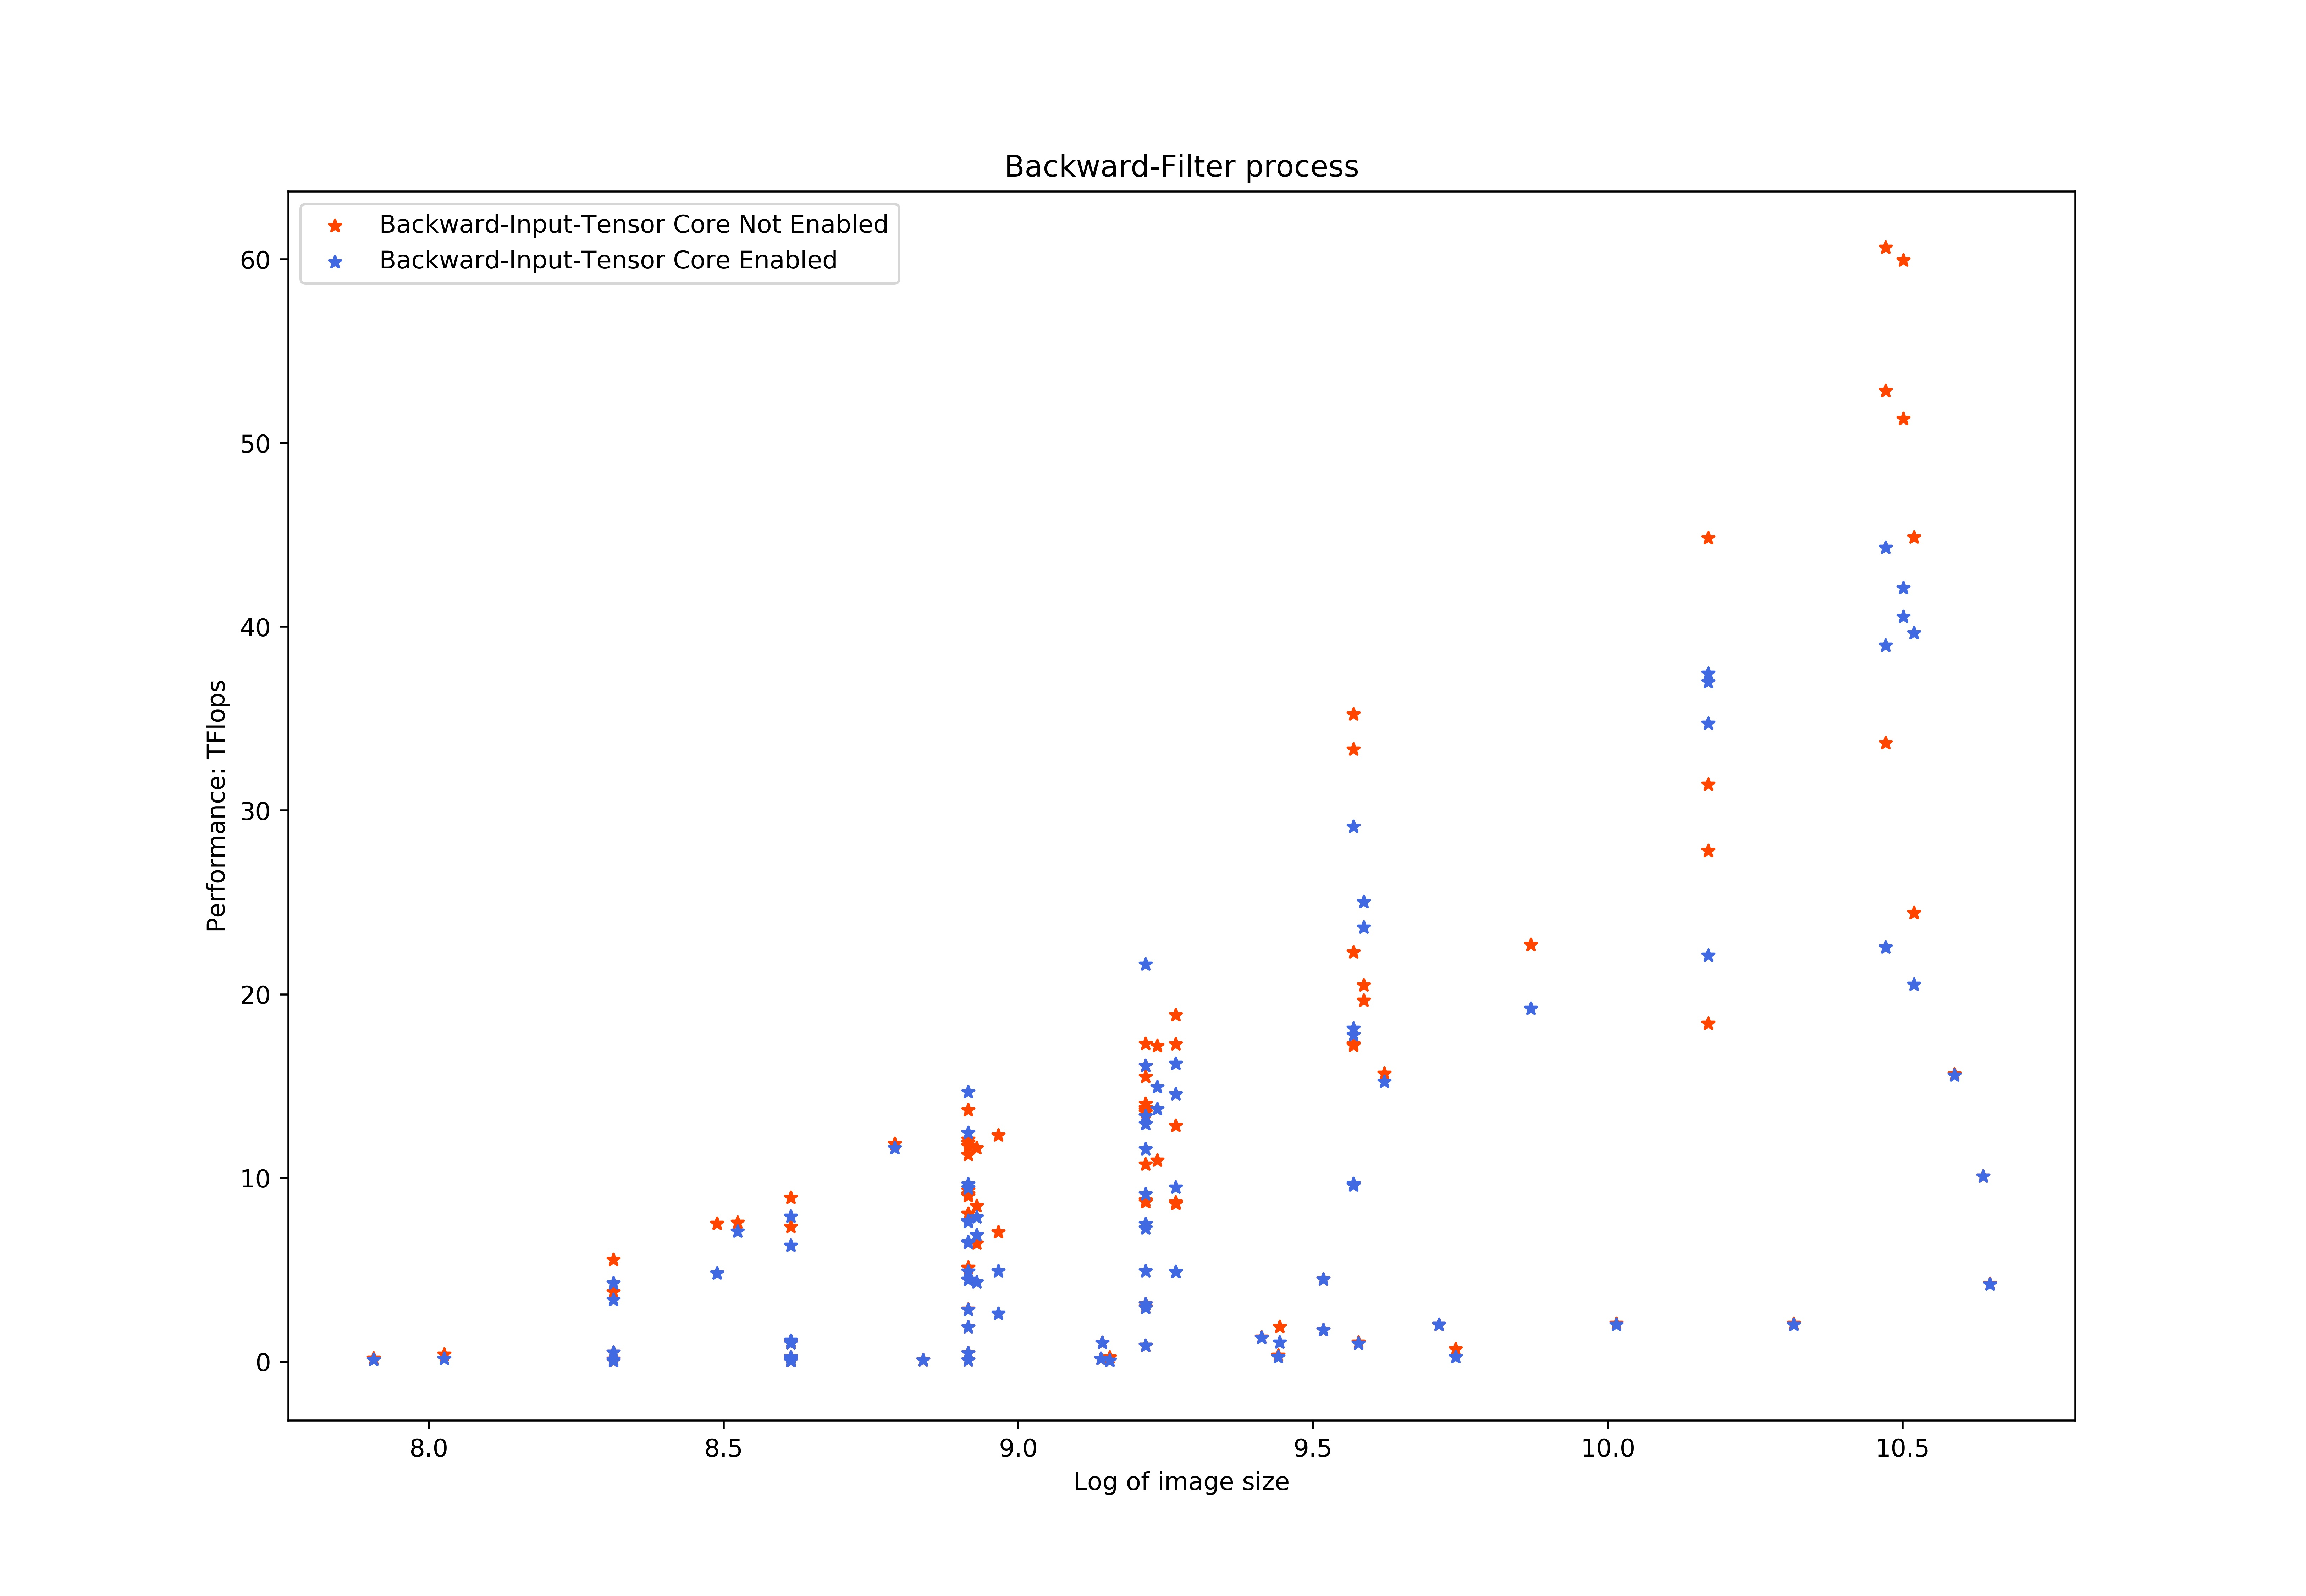
\includegraphics[width=15cm]{figures/CNN-HALF-BWD-FILTER.jpg}
	\renewcommand{\thefigure}{\arabic{section}-\arabic{figure} }
	\renewcommand{\figurename}{图}
	\caption{实验中卷积神经网络不同过程性能(第一部分)}
	\addtocounter{figure}{-1}
	\renewcommand{\thefigure}{\arabic{section}-\arabic{figure} }
	\renewcommand{\figurename}{Figure}
	\caption{Performance of different process in CNN in experiment(Part 1)}
	\label{Fig.CNNPerf-1}
\end{figure}
\begin{figure}
	\centering
	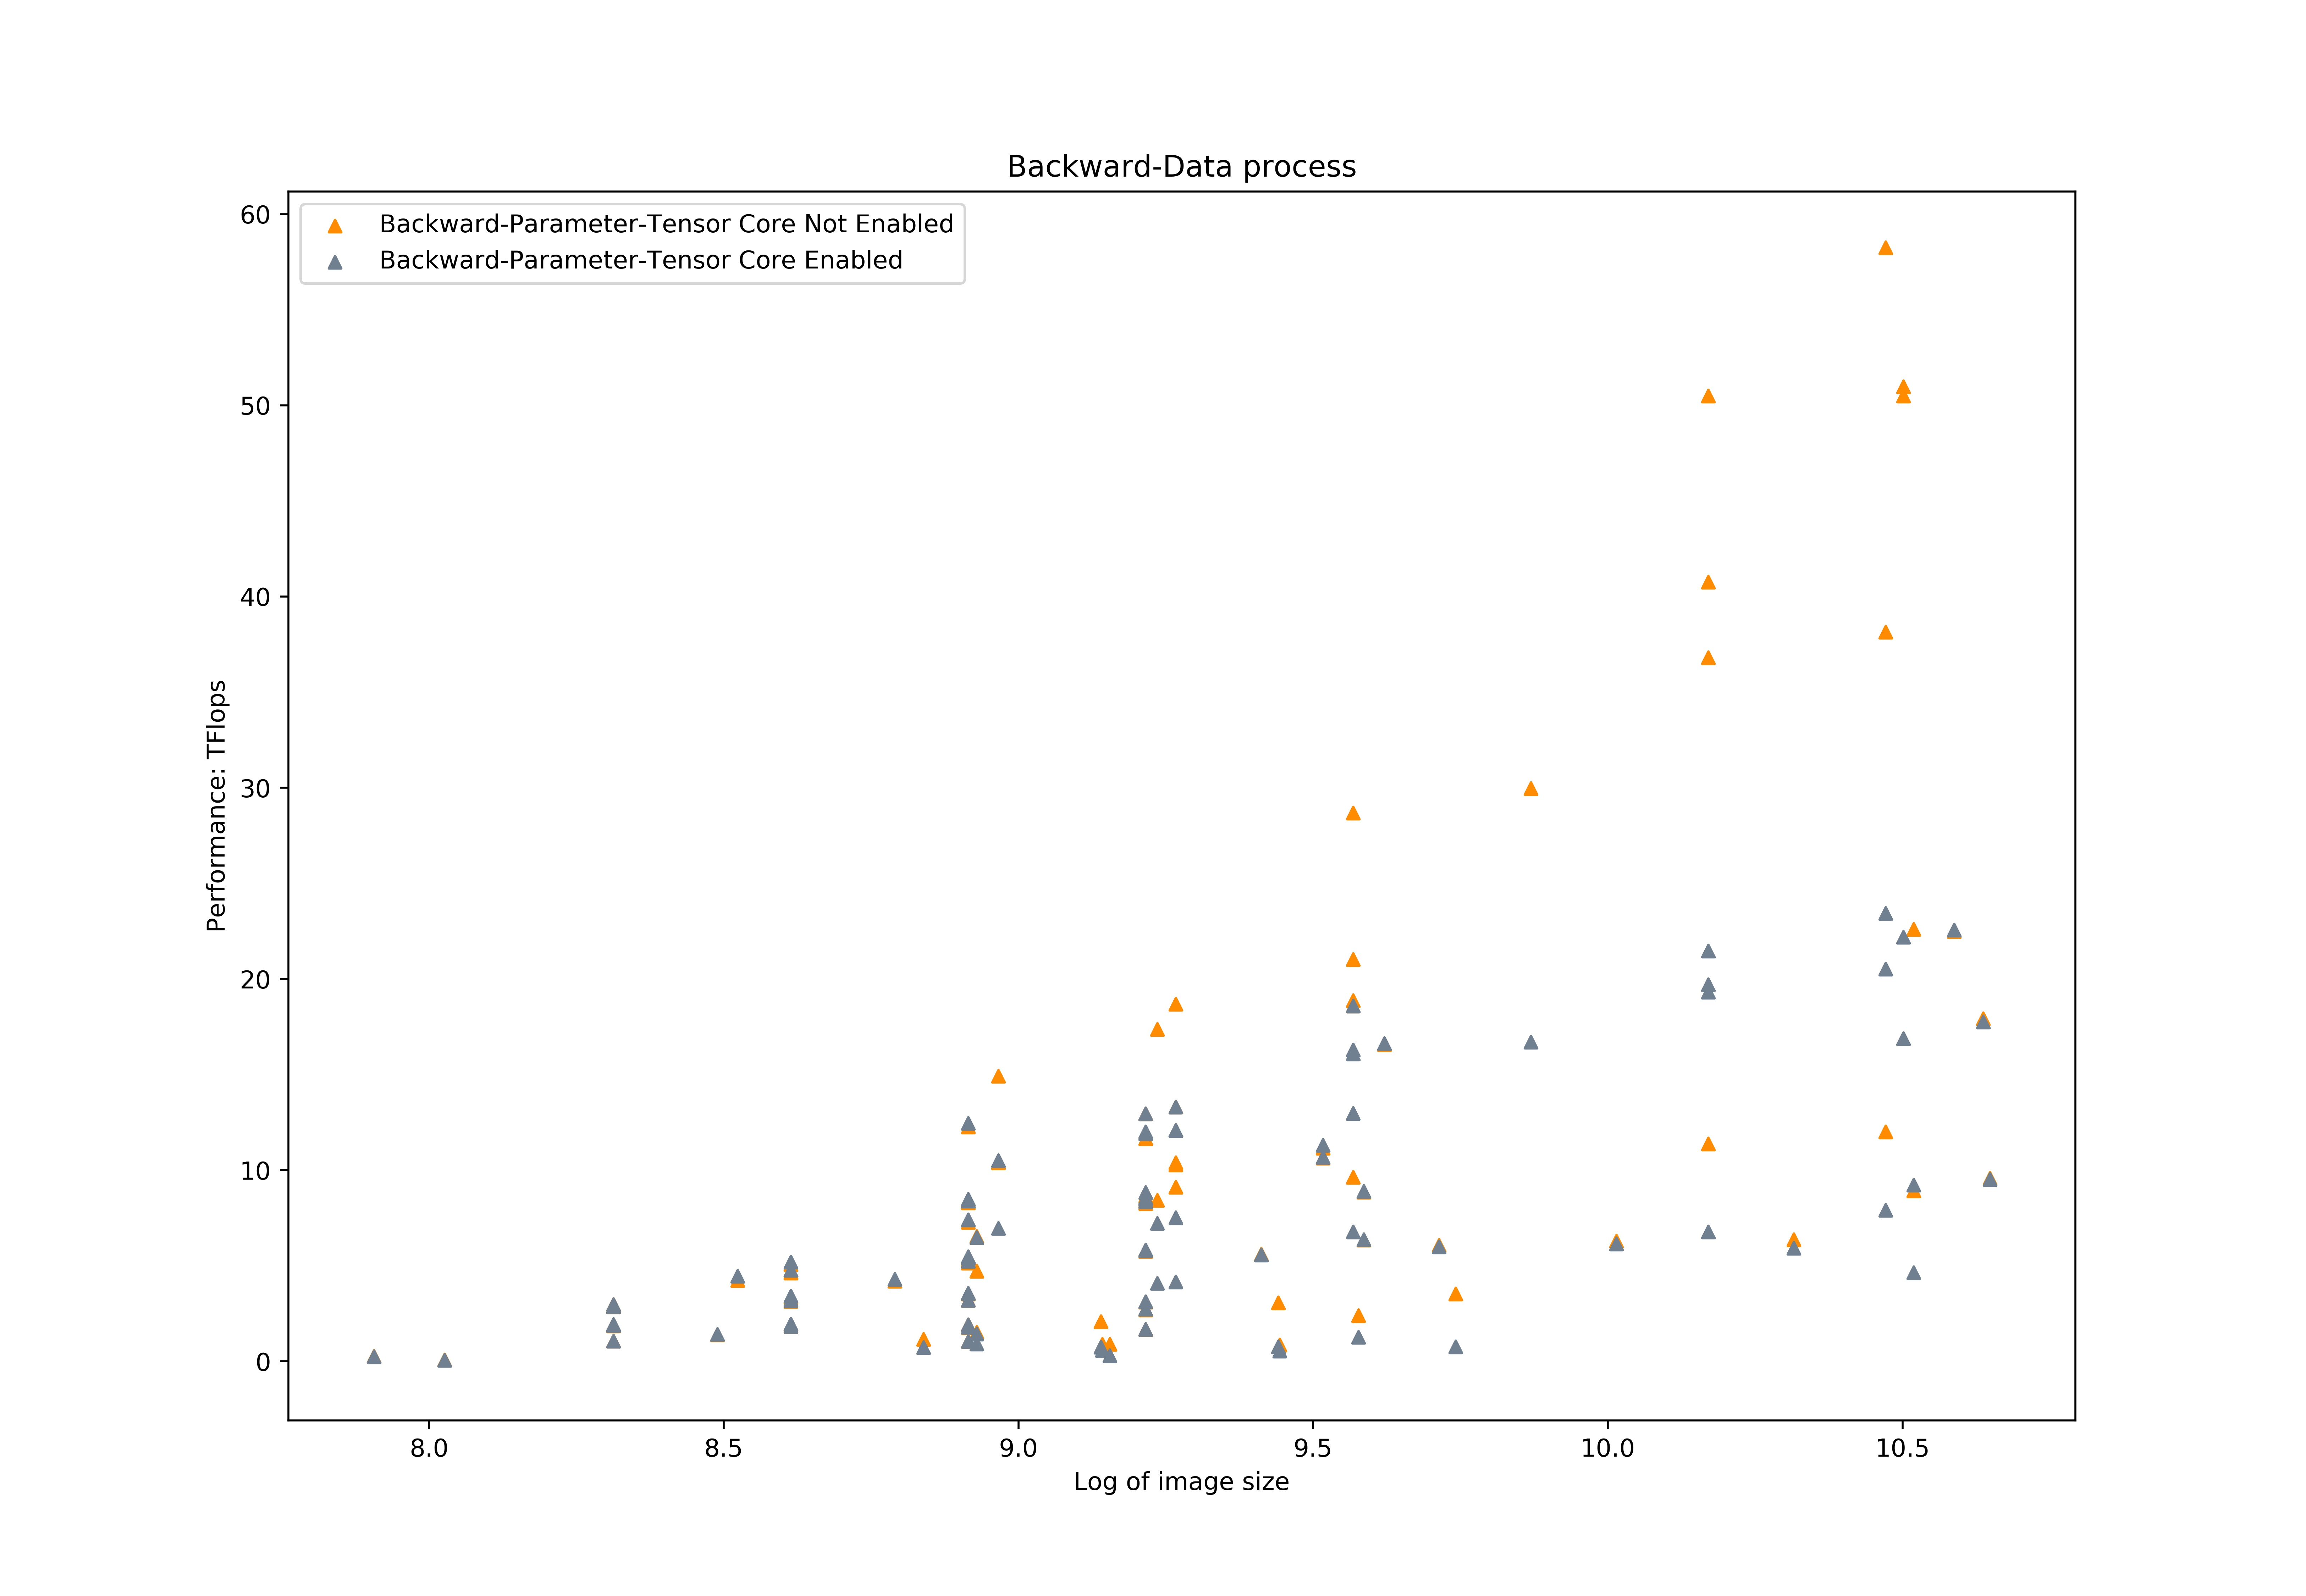
\includegraphics[width=15cm]{figures/CNN-HALF-BWD-DATA.jpg}\\
	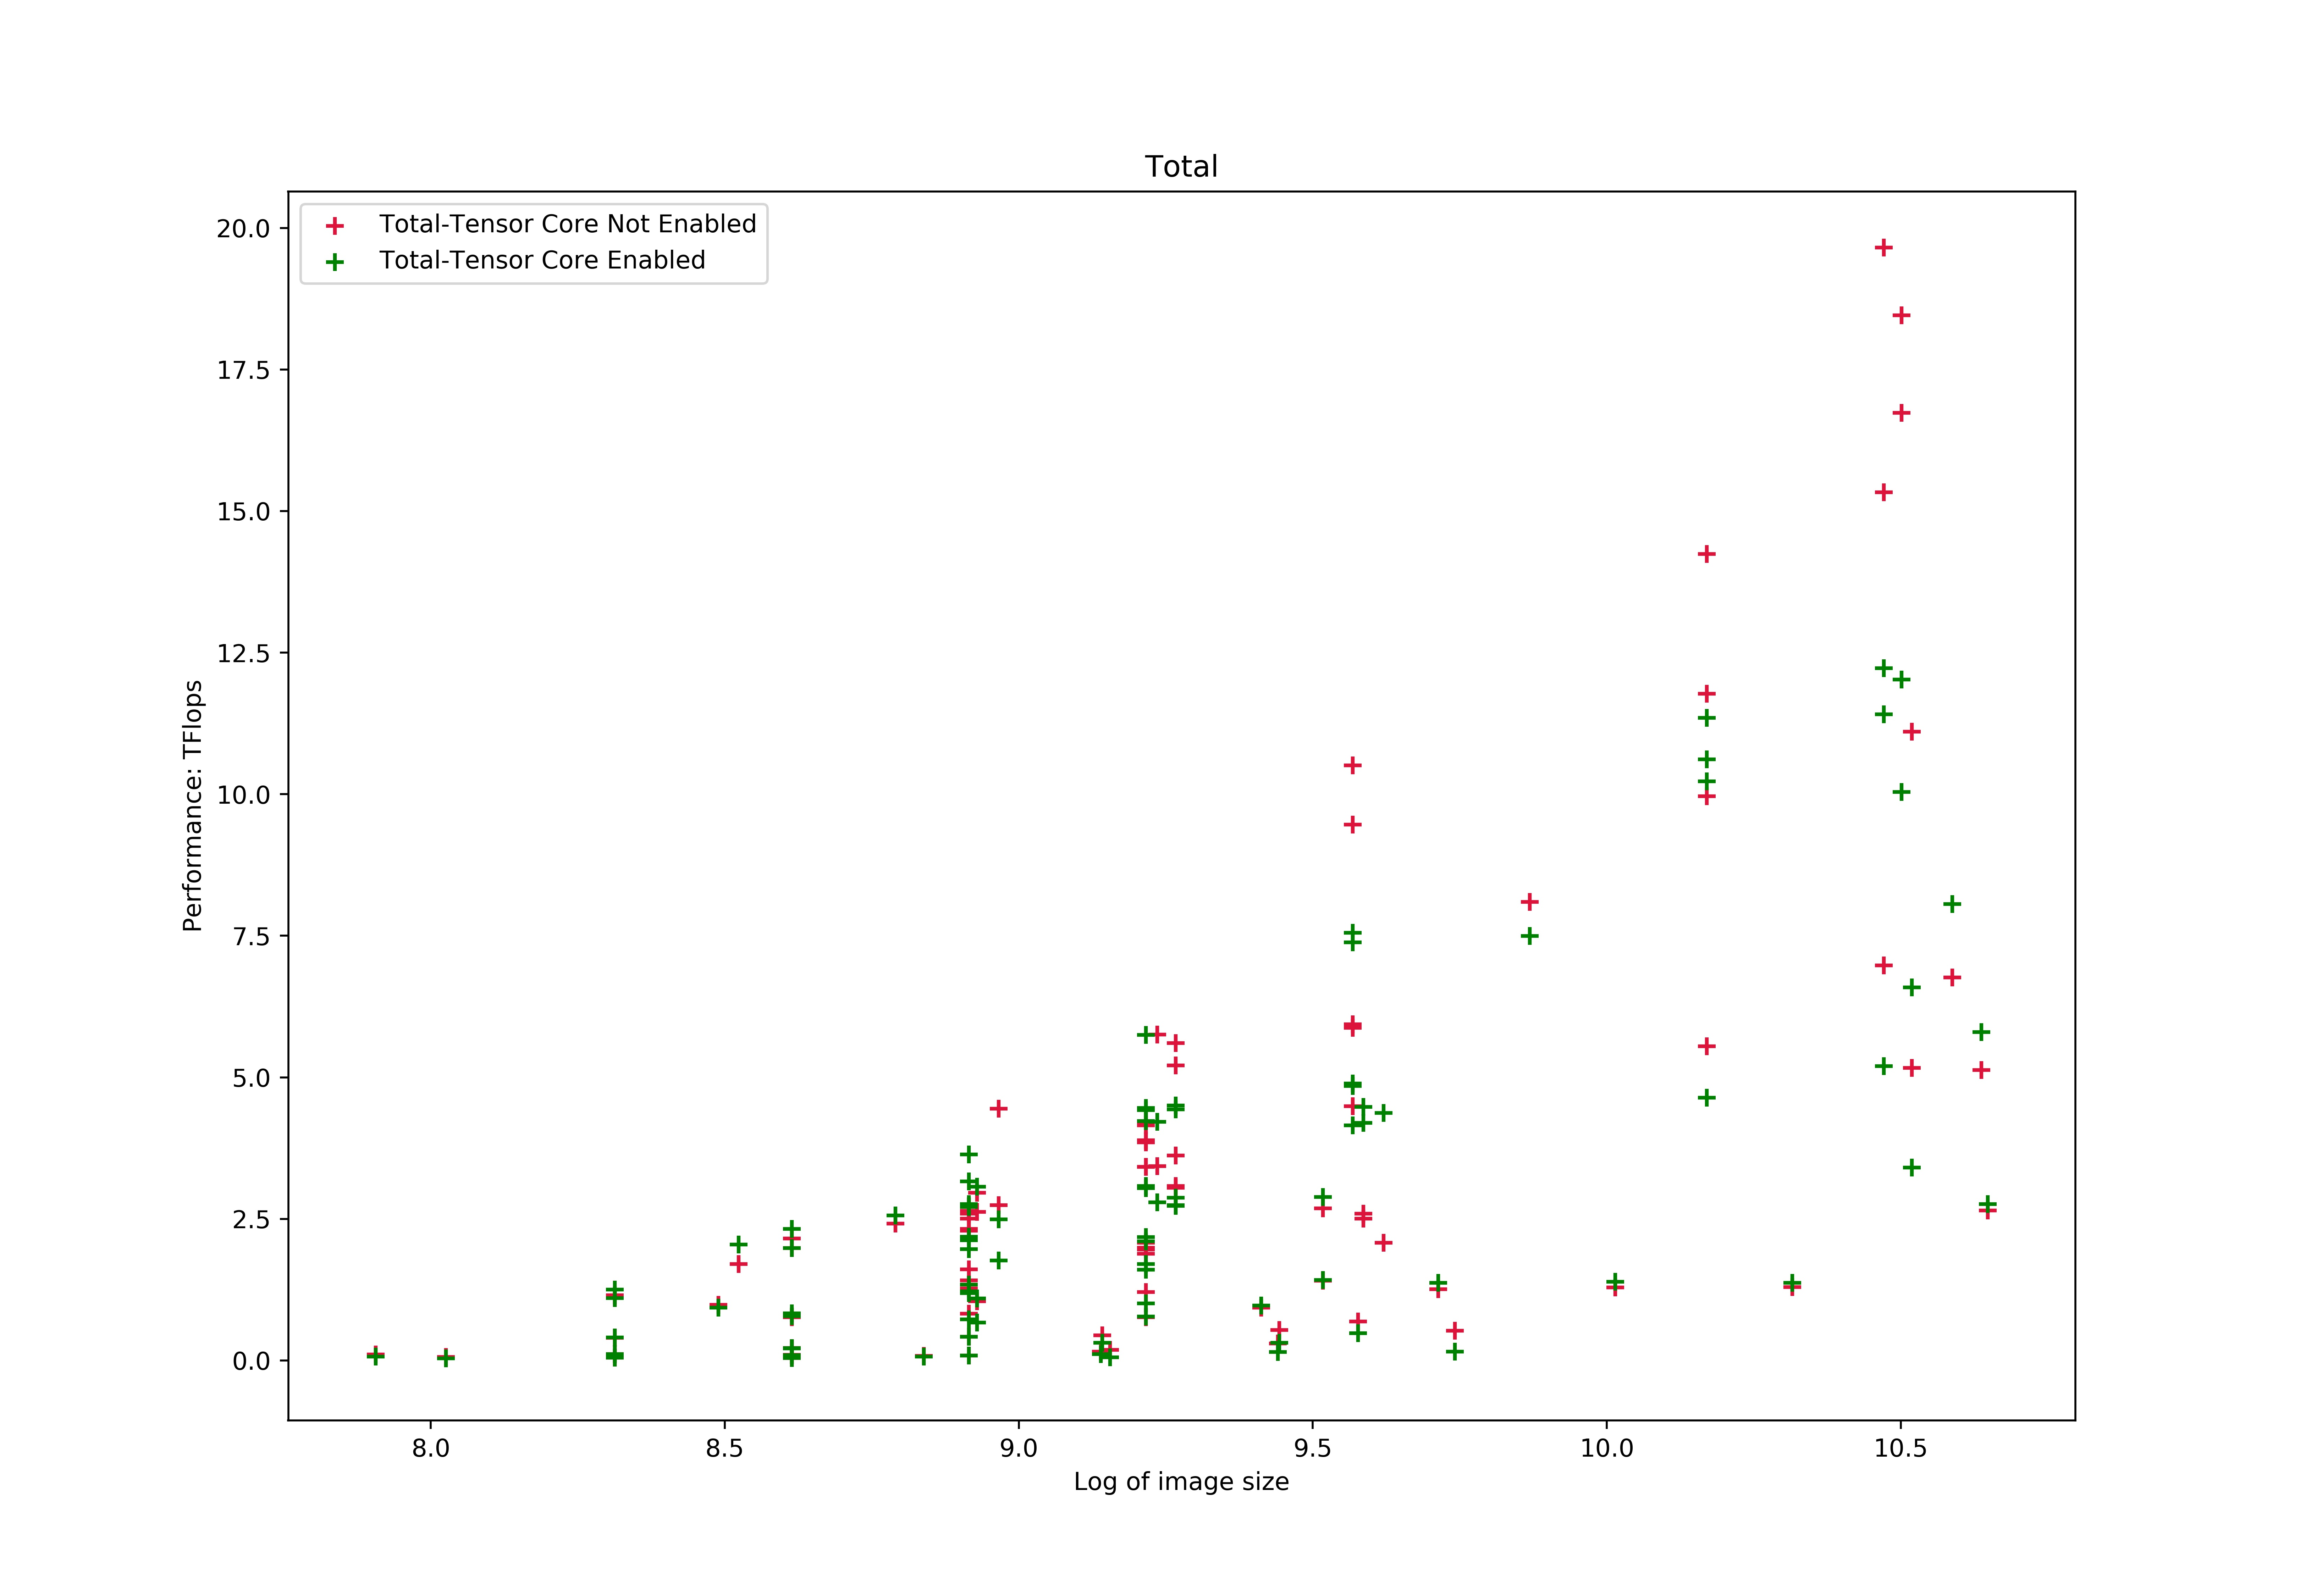
\includegraphics[width=15cm]{figures/CNN-HALF-TOTAL.jpg}
	\renewcommand{\thefigure}{\arabic{section}-\arabic{figure} }
	\renewcommand{\figurename}{图}
	\caption{实验中卷积神经网络不同过程性能(第二部分)}
	\addtocounter{figure}{-1}
	\renewcommand{\thefigure}{\arabic{section}-\arabic{figure} }
	\renewcommand{\figurename}{Figure}
	\caption{Performance of different process in CNN in experiment(Part 2)}
	\label{Fig.CNNPerf-2}
\end{figure}
\par 将卷积神经网络中三个部分的计算整合便得到图 \ref{Fig.CNNPerf3Part}。可以发现开启张量核心时前向传播部分的性能相比反向传播中两个部分的性能高50\%-100\%,而关闭张量核心时三个部分性能相近。
\begin{figure}
	\centering
	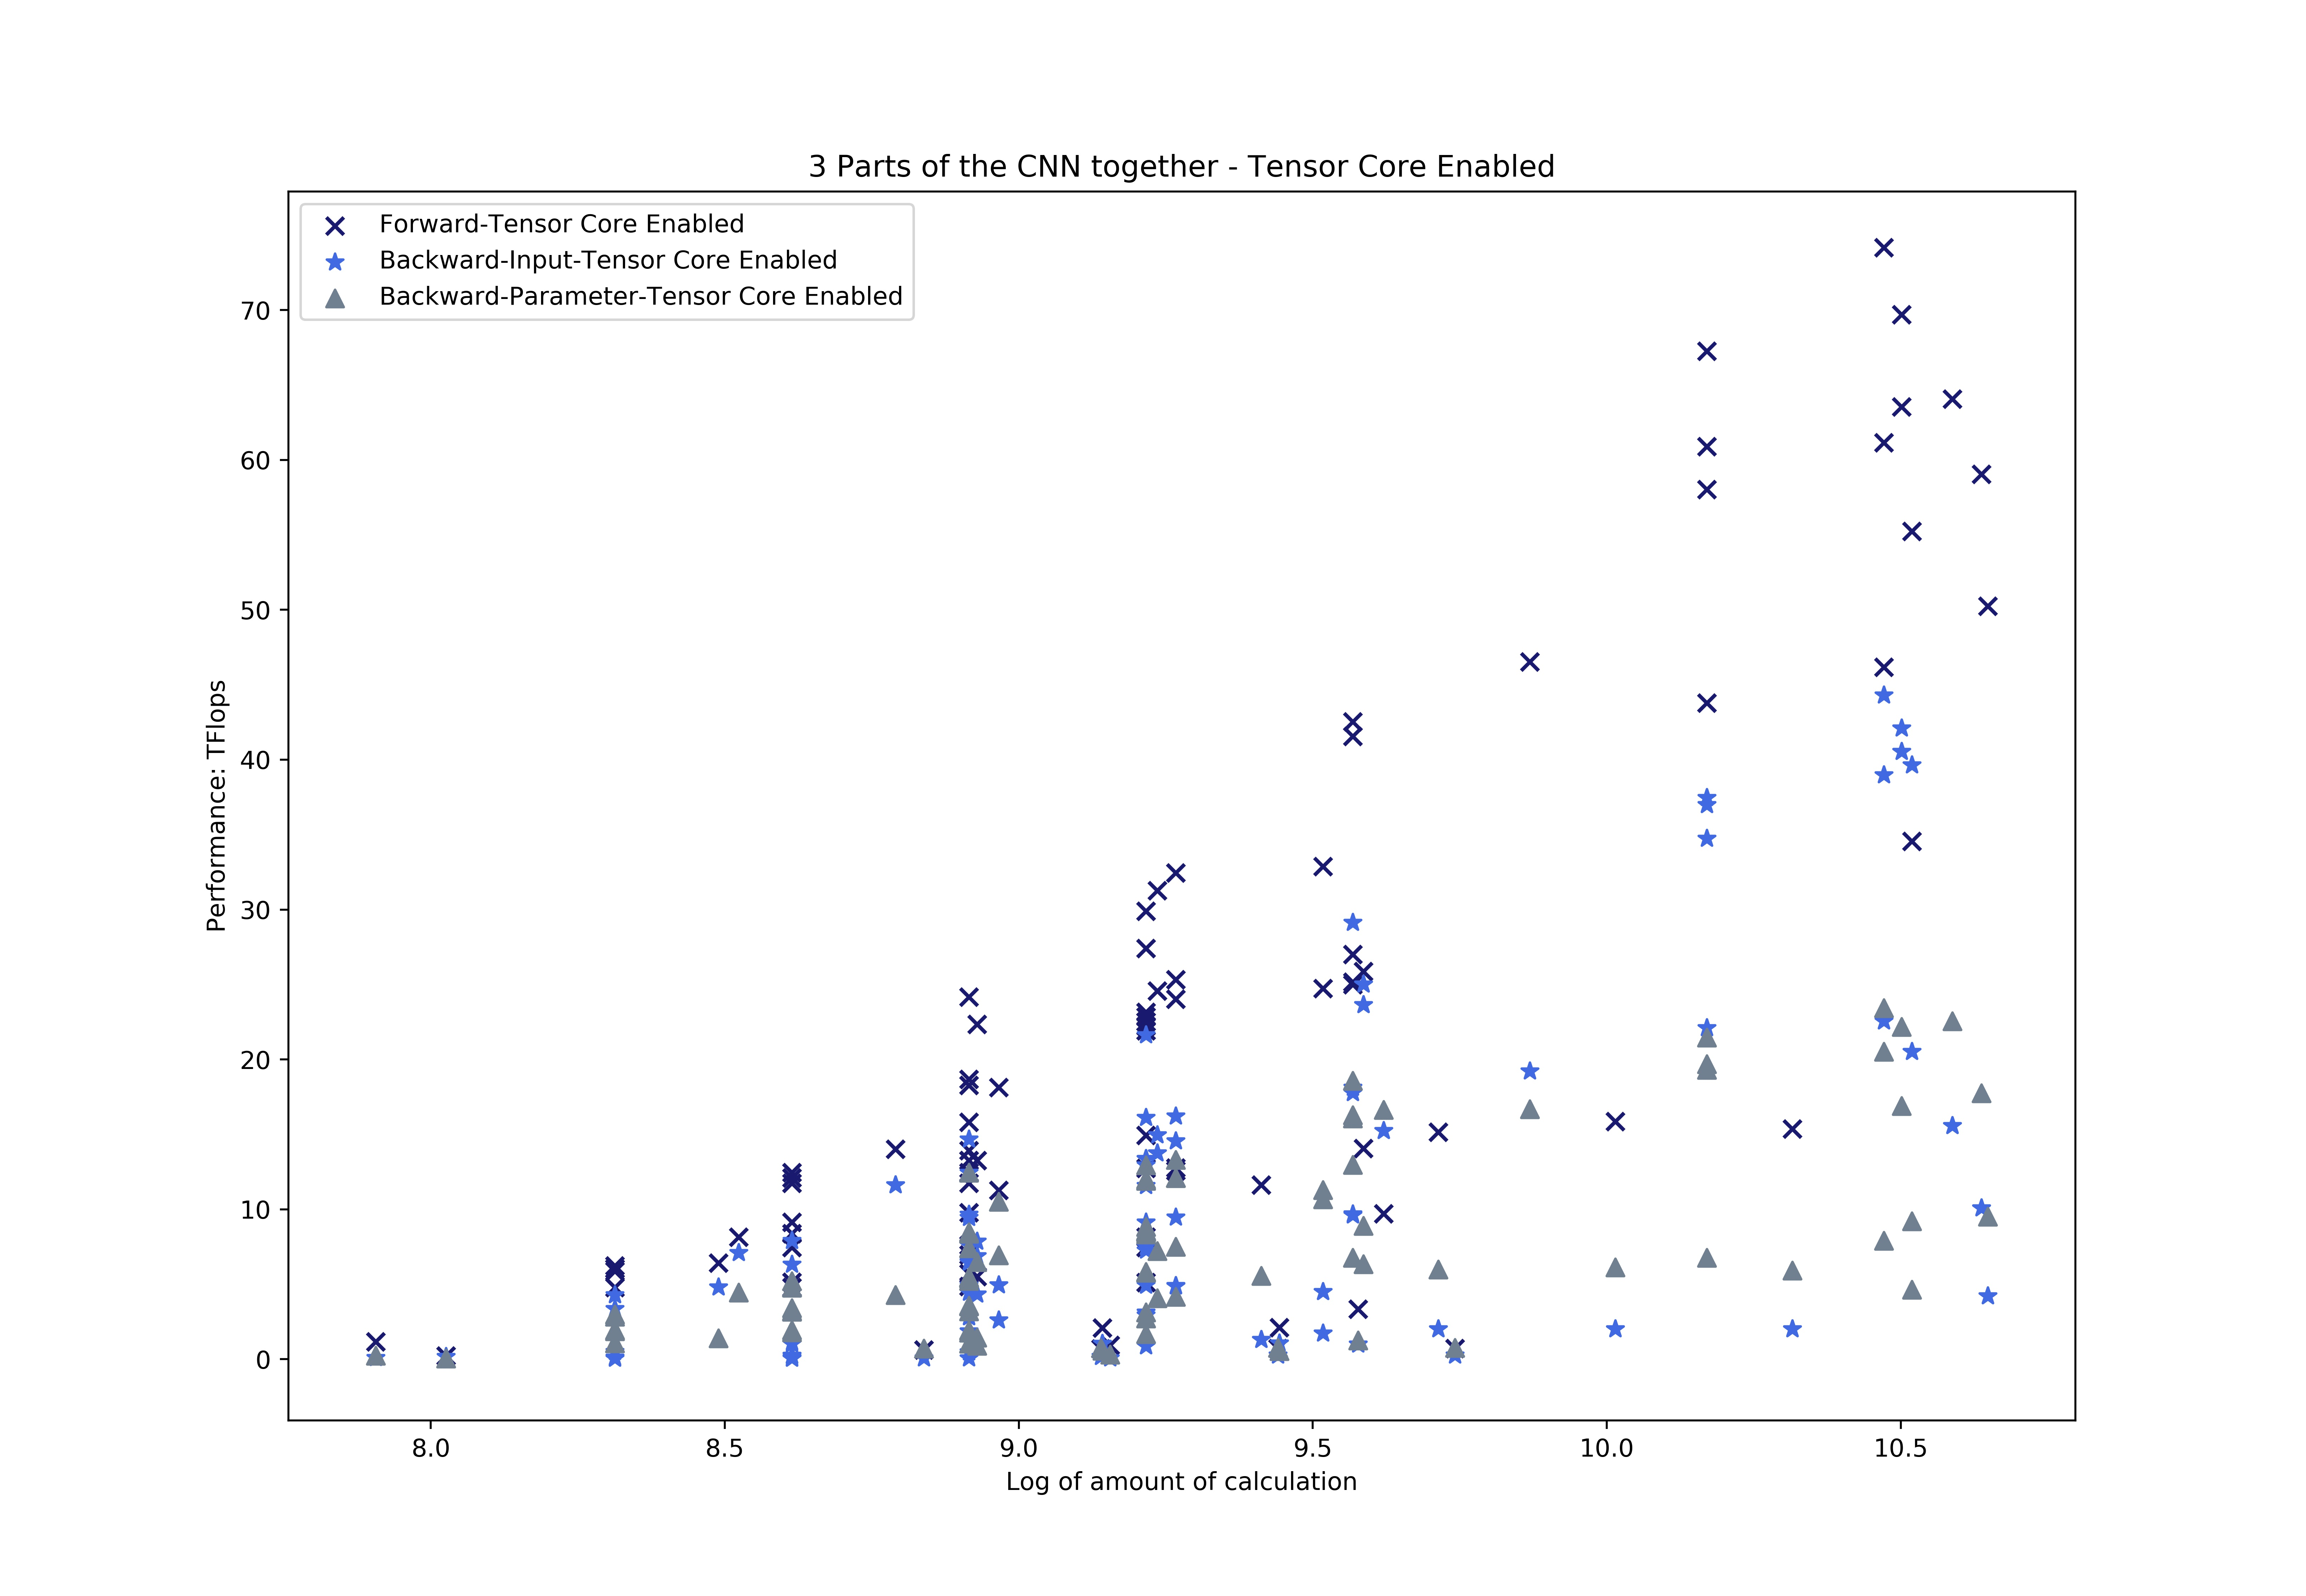
\includegraphics[width=15cm]{figures/CNN-HALF-3PART-TF.jpg}\\
	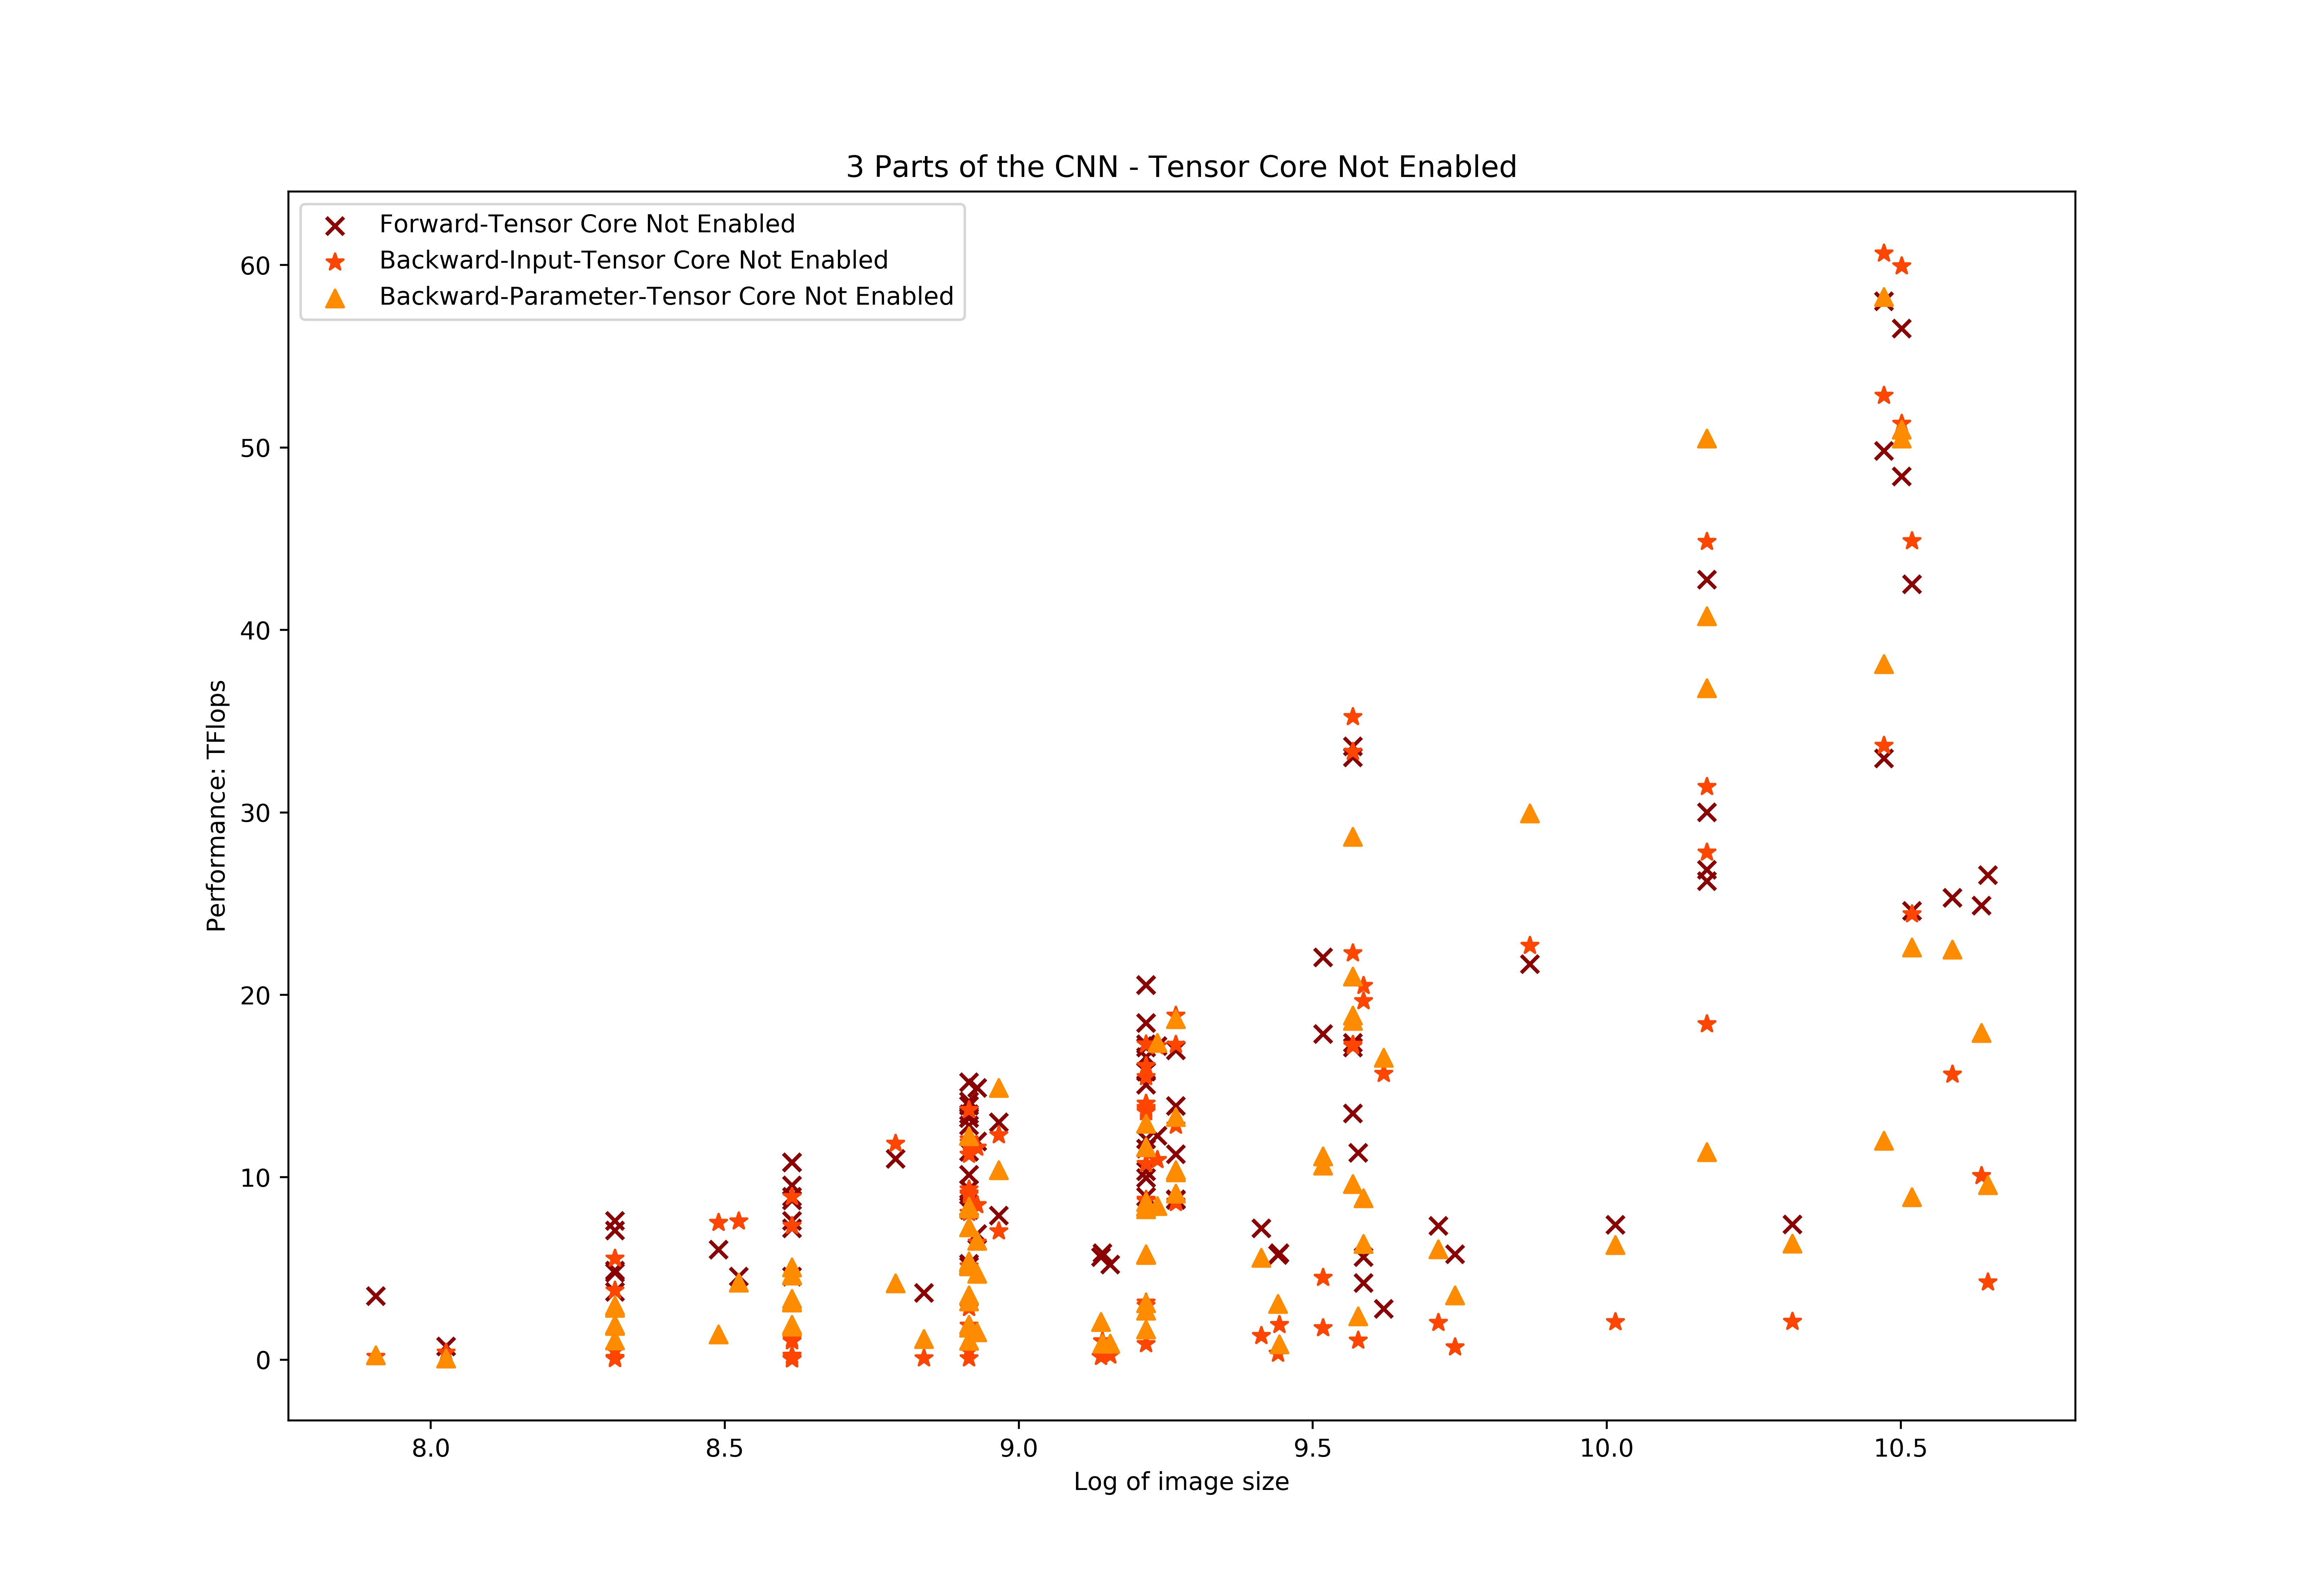
\includegraphics[width=15cm]{figures/CNN-HALF-3PART-NOTF.jpg}
	\renewcommand{\thefigure}{\arabic{section}-\arabic{figure} }
	\renewcommand{\figurename}{图}
	\caption{实验中卷积神经网络不同过程性能整合}
	\addtocounter{figure}{-1}
	\renewcommand{\thefigure}{\arabic{section}-\arabic{figure} }
	\renewcommand{\figurename}{Figure}
	\caption{Collection of performance of different process in CNN in experiment}
	\label{Fig.CNNPerf3Part}
\end{figure}
\paragraph{结果分析}
\par 根据实验结果可以发现,在卷积神经网络中张量核心所能加速的部分较为有限。且尽管根据Benchmark实验中的结果表明计算卷积时,卷积核的尺寸并不会对加速性能造成显著影响,然而神经网络涉及多层卷积,卷积层间需要相连接,从而存在大量参数传播。若开启张量核心对参数传播过程进行加速,由于在卷积神经网络的前向传播中,每一层图像尺寸、神经元连接规模都会被输入图像尺寸、卷积核尺寸、边缘填充尺寸、卷积核步进等因素影响,即使原始输入尺寸满足张量核心的理想需求,在卷积之后也很难保证,故开启张量核心后前向传播部分提升也有限。而如图 \ref{Fig.CNNPerf3Part}中所示,开启张量核心后三部分性能差距较大,这也是导致图 \ref{Fig.CNNPerf-2}中总体性能较差的原因。
\par 而在反向传播的两个部分的实验中,采用了NSight与nvprof对其运行进行观察。由于是一个完整的神经网络,nvprof所得的报告条目较多,且有些条目并不必要。这里选取神经网络中典型的操作:ReLU作为除卷积、矩阵乘加运算外其他运算的代表,考察开启和不开启张量核心时该操作花费的时间,如表 \ref{table-RELU}所示。开启张量核心后,会使用针对新架构的API(turing)进行运算,然而,不仅调用的API数量明显增加,基于图灵架构的API的运行时间仍更长。可以推断出,由于完整神经网络中存在的其他运算较多,而在第二章提到过张量核心使用的指令流水线(M-pipe)与其他算术指令的流水线是互斥的,这就导致张量核心指令与一般算数指令在同一流多处理器中无法同时执行,张量核心在以较低效率执行不适合它的操作的同时还阻塞了其他算术运算的进行。
\begin{table}
	\centering
	\renewcommand{\thetable}{\arabic{section}-\arabic{table} }
	\renewcommand{\tablename}{表}
	\caption{ReLU相关运算API及耗时}
	\addtocounter{table}{-1}
	\renewcommand{\thetable}{\arabic{section}-\arabic{table} }
	\renewcommand{\tablename}{Table}
	\caption{APIs and time spent on ReLU related calculation}
	\begin{tabular}{clc}
		\toprule
		张量核心 & API	&	时间(ms)\\
		\midrule
		ON & turing\_h1688cudnn\_256x64\_sliced1x2\_ldg8\_relu\_exp\_interior\_nhwc\_tn & 514.85\\
		   & turing\_h1688cudnn\_256x64\_sliced1x2\_ldg8\_relu\_exp\_small\_nhwc\_tn & 158.85\\
		   & turing\_h1688cudnn\_256x128\_ldg8\_relu\_exp\_small\_nhwc\_tn & 88.135\\
		   & turing\_h1688cudnn\_128x128\_ldg8\_relu\_exp\_small\_nhwc\_tn & 53.434\\
		   & turing\_h1688cudnn\_128x128\_ldg8\_relu\_exp\_interior\_nhwc\_tn & 32.362\\
		   & turing\_h1688cudnn\_256x64\_sliced1x2\_ldg8\_relu\_exp\_medium\_nhwc\_tn & 29.385\\
		   & volta\_hcudnn\_128x128\_relu\_small\_nn\_v1 & 27.248\\
		   & volta\_hcudnn\_128x128\_relu\_interior\_nn\_v1 & 19.293\\
		   & turing\_h1688cudnn\_256x128\_ldg8\_relu\_exp\_interior\_nhwc\_tn & 2.5632\\
		   & volta\_hcudnn\_128x128\_relu\_medium\_nn\_v1 & 0.7397\\
		\midrule
		OFF& volta\_hcudnn\_128x128\_relu\_interior\_nn\_v1 & 307.43\\
		   & volta\_hcudnn\_128x128\_relu\_small\_nn\_v1 & 292.25\\
		   & volta\_hcudnn\_128x128\_relu\_medium\_nn\_v1 & 10.183\\
		\bottomrule
	\end{tabular} \label{table-RELU} 
\end{table}
\par 结合上文对卷积性能的评估,又考虑到实验中使用的数据集中有大量$ 10^2 $规模的图像,而cudnn中选择的卷积方式中包括直接方法均并不使用纹理内存。由于cuDNN将底层运算进行了封装,故无法在cudnn上将直接方法调整为使用纹理内存。故首先本文选择将cuDNN卷积计算方法更换为直接方法。之后采用原生CUDA代码而不包含cuDNN库的方式搭建卷积神经网络,考察使用纹理内存优化的直接方法相比不适用纹理内存优化的直接方法的运算速度提升幅度,原生CUDA代码参考了Eric Yuan的实现\cite{ERICYUAN}。
\par 将cuDNN中卷积计算方法更换为直接方法后的性能如图 \ref{Fig.CNNDIRECT}所示。可以发现在图像尺寸较小的情况下,使用直接方法优于使用快速傅里叶变换的方法。然而使用张量核心的方法性能优势依旧明显,仅在图像尺寸极小的情况下落后于直接方法,这也与上文提实验中的现象相符。其原因为卷积神经网络前向传播过程中,除卷积计算,根据权重进行前向传播也是主要计算。这一部分使用张量核心优势较大。在实际使用中,若硬件支持张量核心,应尽可能选用张量核心进行前向传播计算;然而,若设备不支持张量核心,在图像尺寸较小时可以选用直接方法进行计算,所以在反向传播过程中开启张量核心反而会导致性能下降。
\begin{figure}
	\centering
	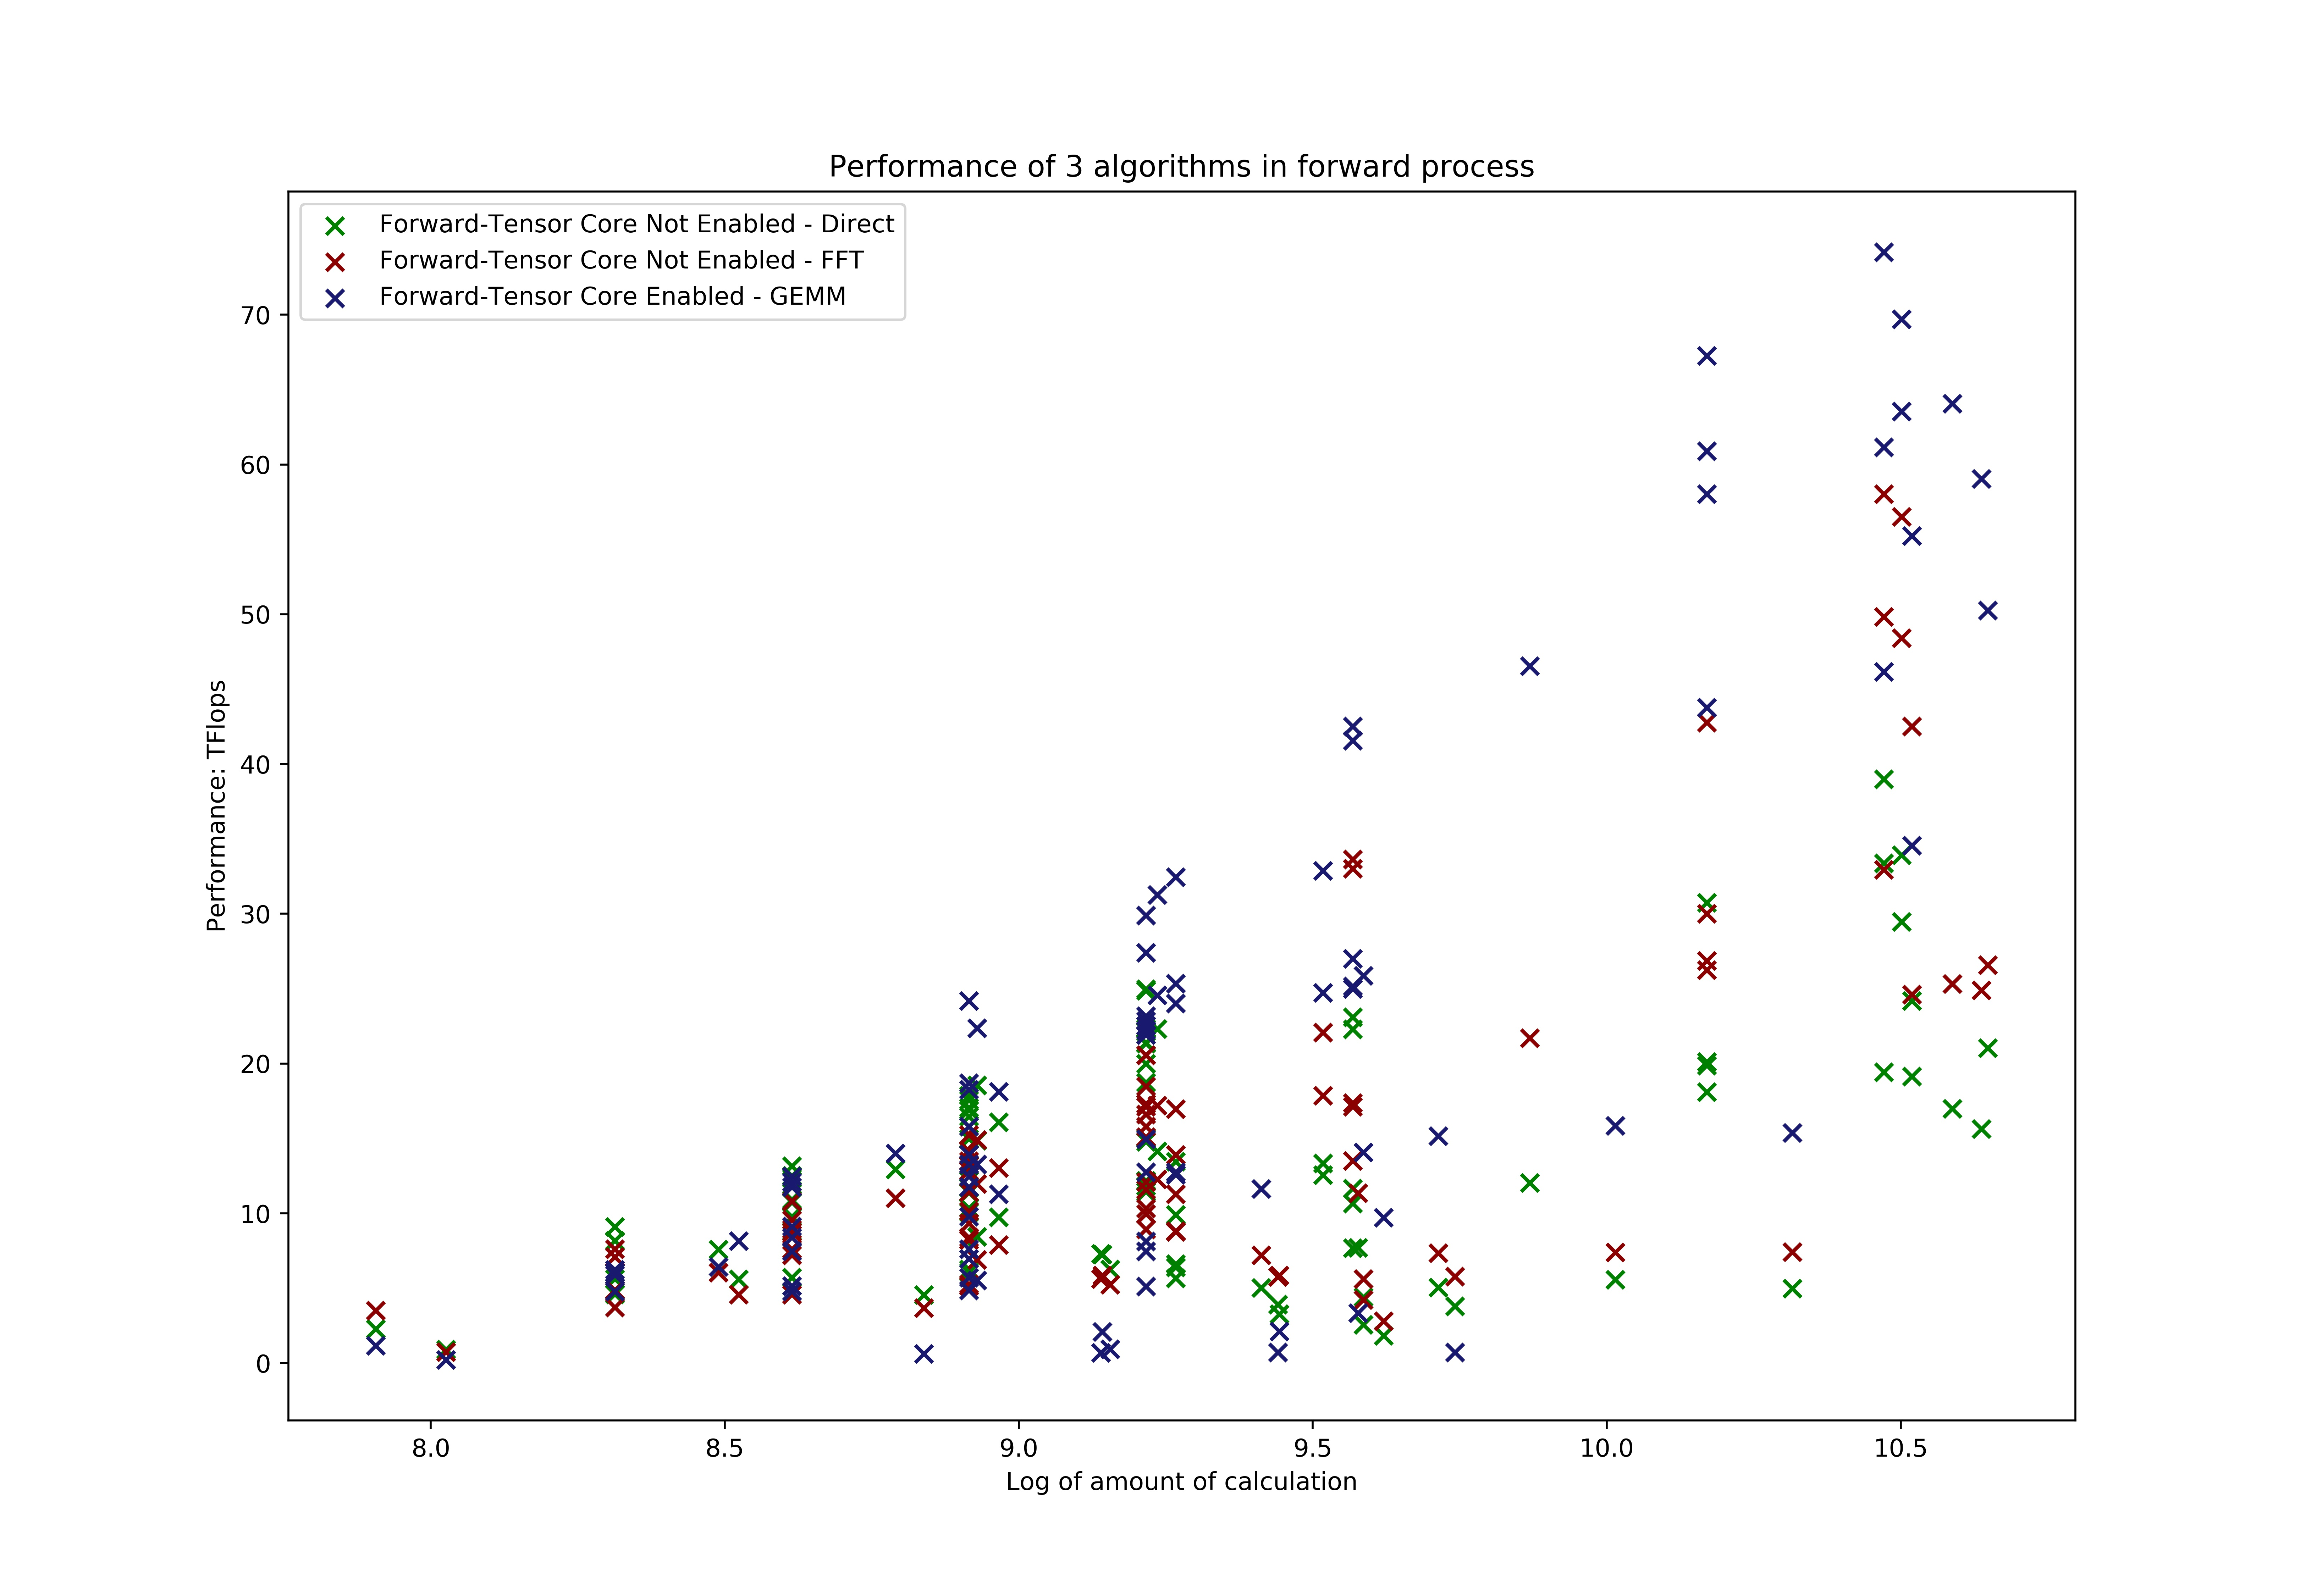
\includegraphics[width=15cm]{figures/CNN-HALF-3ALGOFWD.jpg}
	\renewcommand{\thefigure}{\arabic{section}-\arabic{figure} }
	\renewcommand{\figurename}{图}
	\caption{使用cuDNN中直接计算方法的性能对比}
	\addtocounter{figure}{-1}
	\renewcommand{\thefigure}{\arabic{section}-\arabic{figure} }
	\renewcommand{\figurename}{Figure}
	\caption{Performance of DIRECT algorithm in cuDNN}
	\label{Fig.CNNDIRECT}
\end{figure}
\par 在基于原生CUDA代码搭建的卷积神经网络中,图 \ref{Fig.TEXVSSHARED}显示了使用纹理内存优化后的网络前向传播性能与原始代码的前向传播性能比较。根据前文的实验结果,纹理内存仅在小尺寸图像优势较大,故这里仅考察小图像时两者的性能,且由于未使用cuDNN,代码无法使GPU设备满载,故有意义的实验结果仅为比较两者的性能提升幅度。根据图中实验结果所示,在图像尺寸极小时,使用纹理内存和全局内存区别不大,而随着图像尺寸增加,纹理内存优化后的前向传播性能稳定在使用全局内存的1.5-1.7倍,而全局内存仍有增长的趋势,这也与上文实验中稍大的图像上全局内存表现逐渐优于纹理内存相符;同时,上文卷积实验中使用纹理内存的性能在小尺寸图像相对全局内存能够超过2倍,约2.5倍,然而由于前向传播中还有其他运算,这一结果也符合预期。
\par 图 \ref{Fig.TexCode}是对卷积部分使用纹理内存优化替代原代码中的g\_ConvCFM\_feedforward\_shared()函数后的代码片段。由于行列卷积在上文的实验中差别不大,且代码重复率高,故只展示行卷积代码段。
\begin{figure}
	\centering
	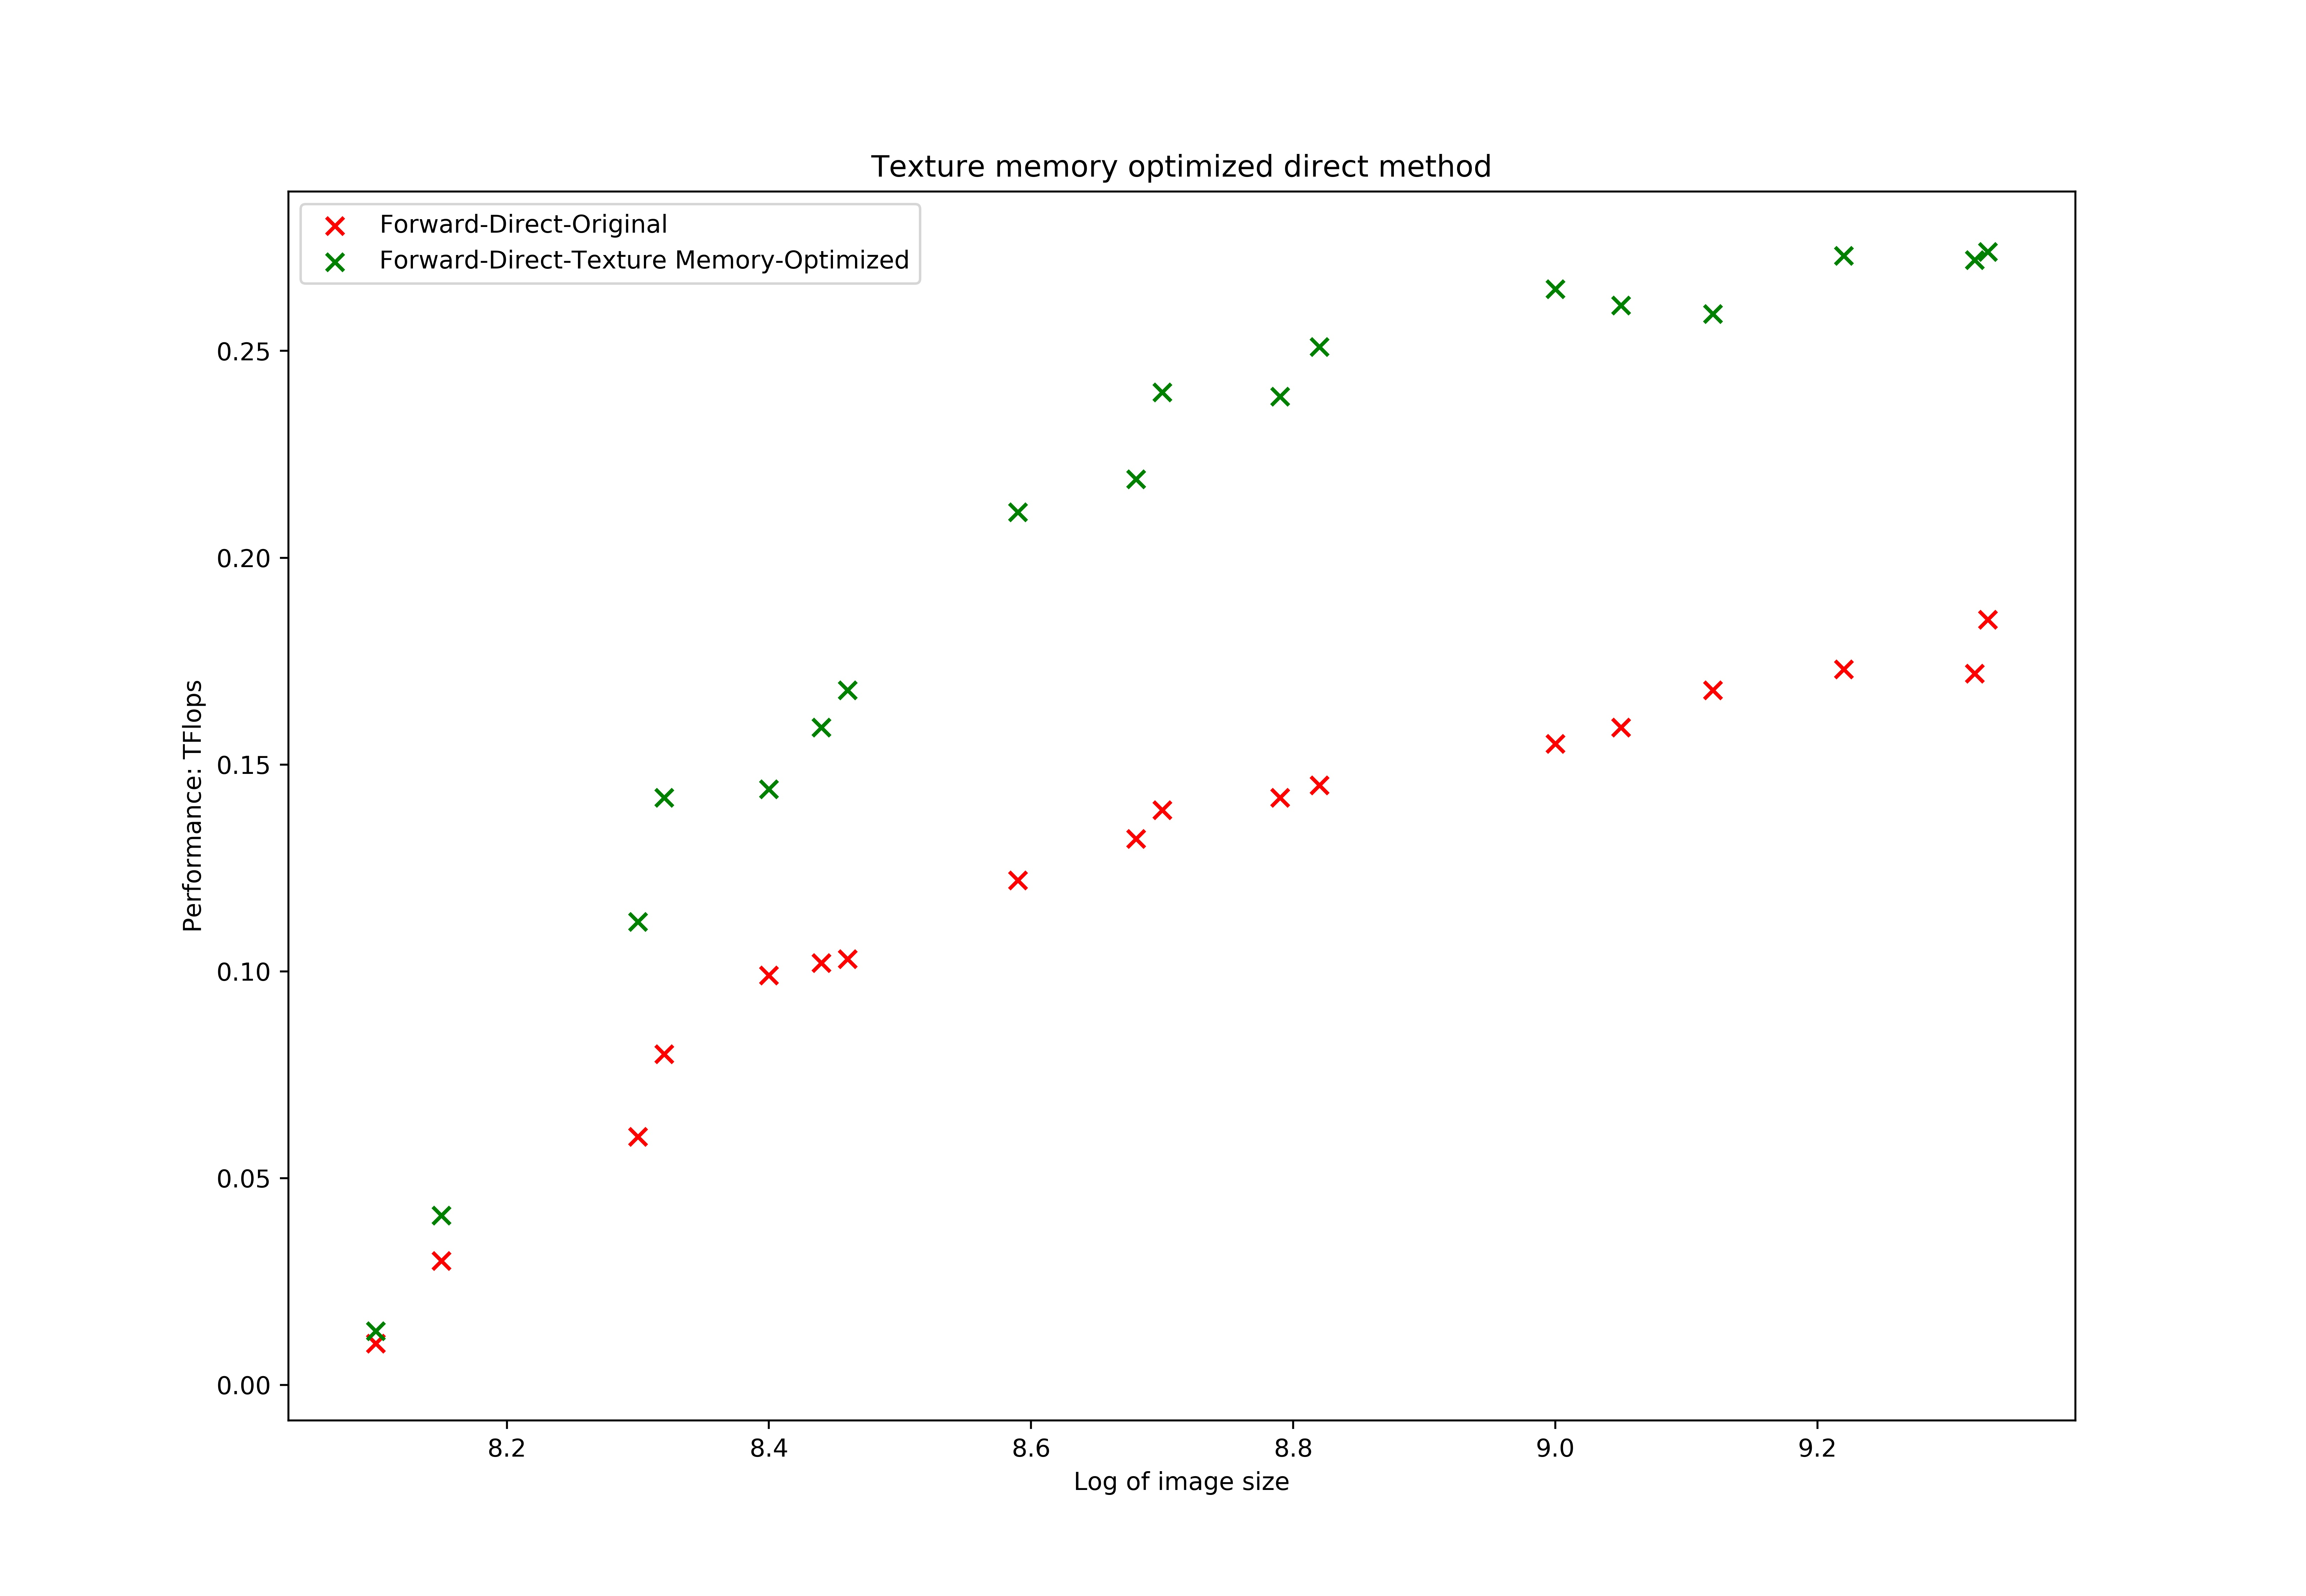
\includegraphics[width=15cm]{figures/CNN-HALF-TEXOPT.jpg}
	\renewcommand{\thefigure}{\arabic{section}-\arabic{figure} }
	\renewcommand{\figurename}{图}
	\caption{使用纹理内存优化的小尺寸图象前向传播性能}
	\addtocounter{figure}{-1}
	\renewcommand{\thefigure}{\arabic{section}-\arabic{figure} }
	\renewcommand{\figurename}{Figure}
	\caption{Performance of forward on small image optimized by texture memory}
	\label{Fig.TEXVSSHARED}
\end{figure}
\begin{figure}
	\centering
	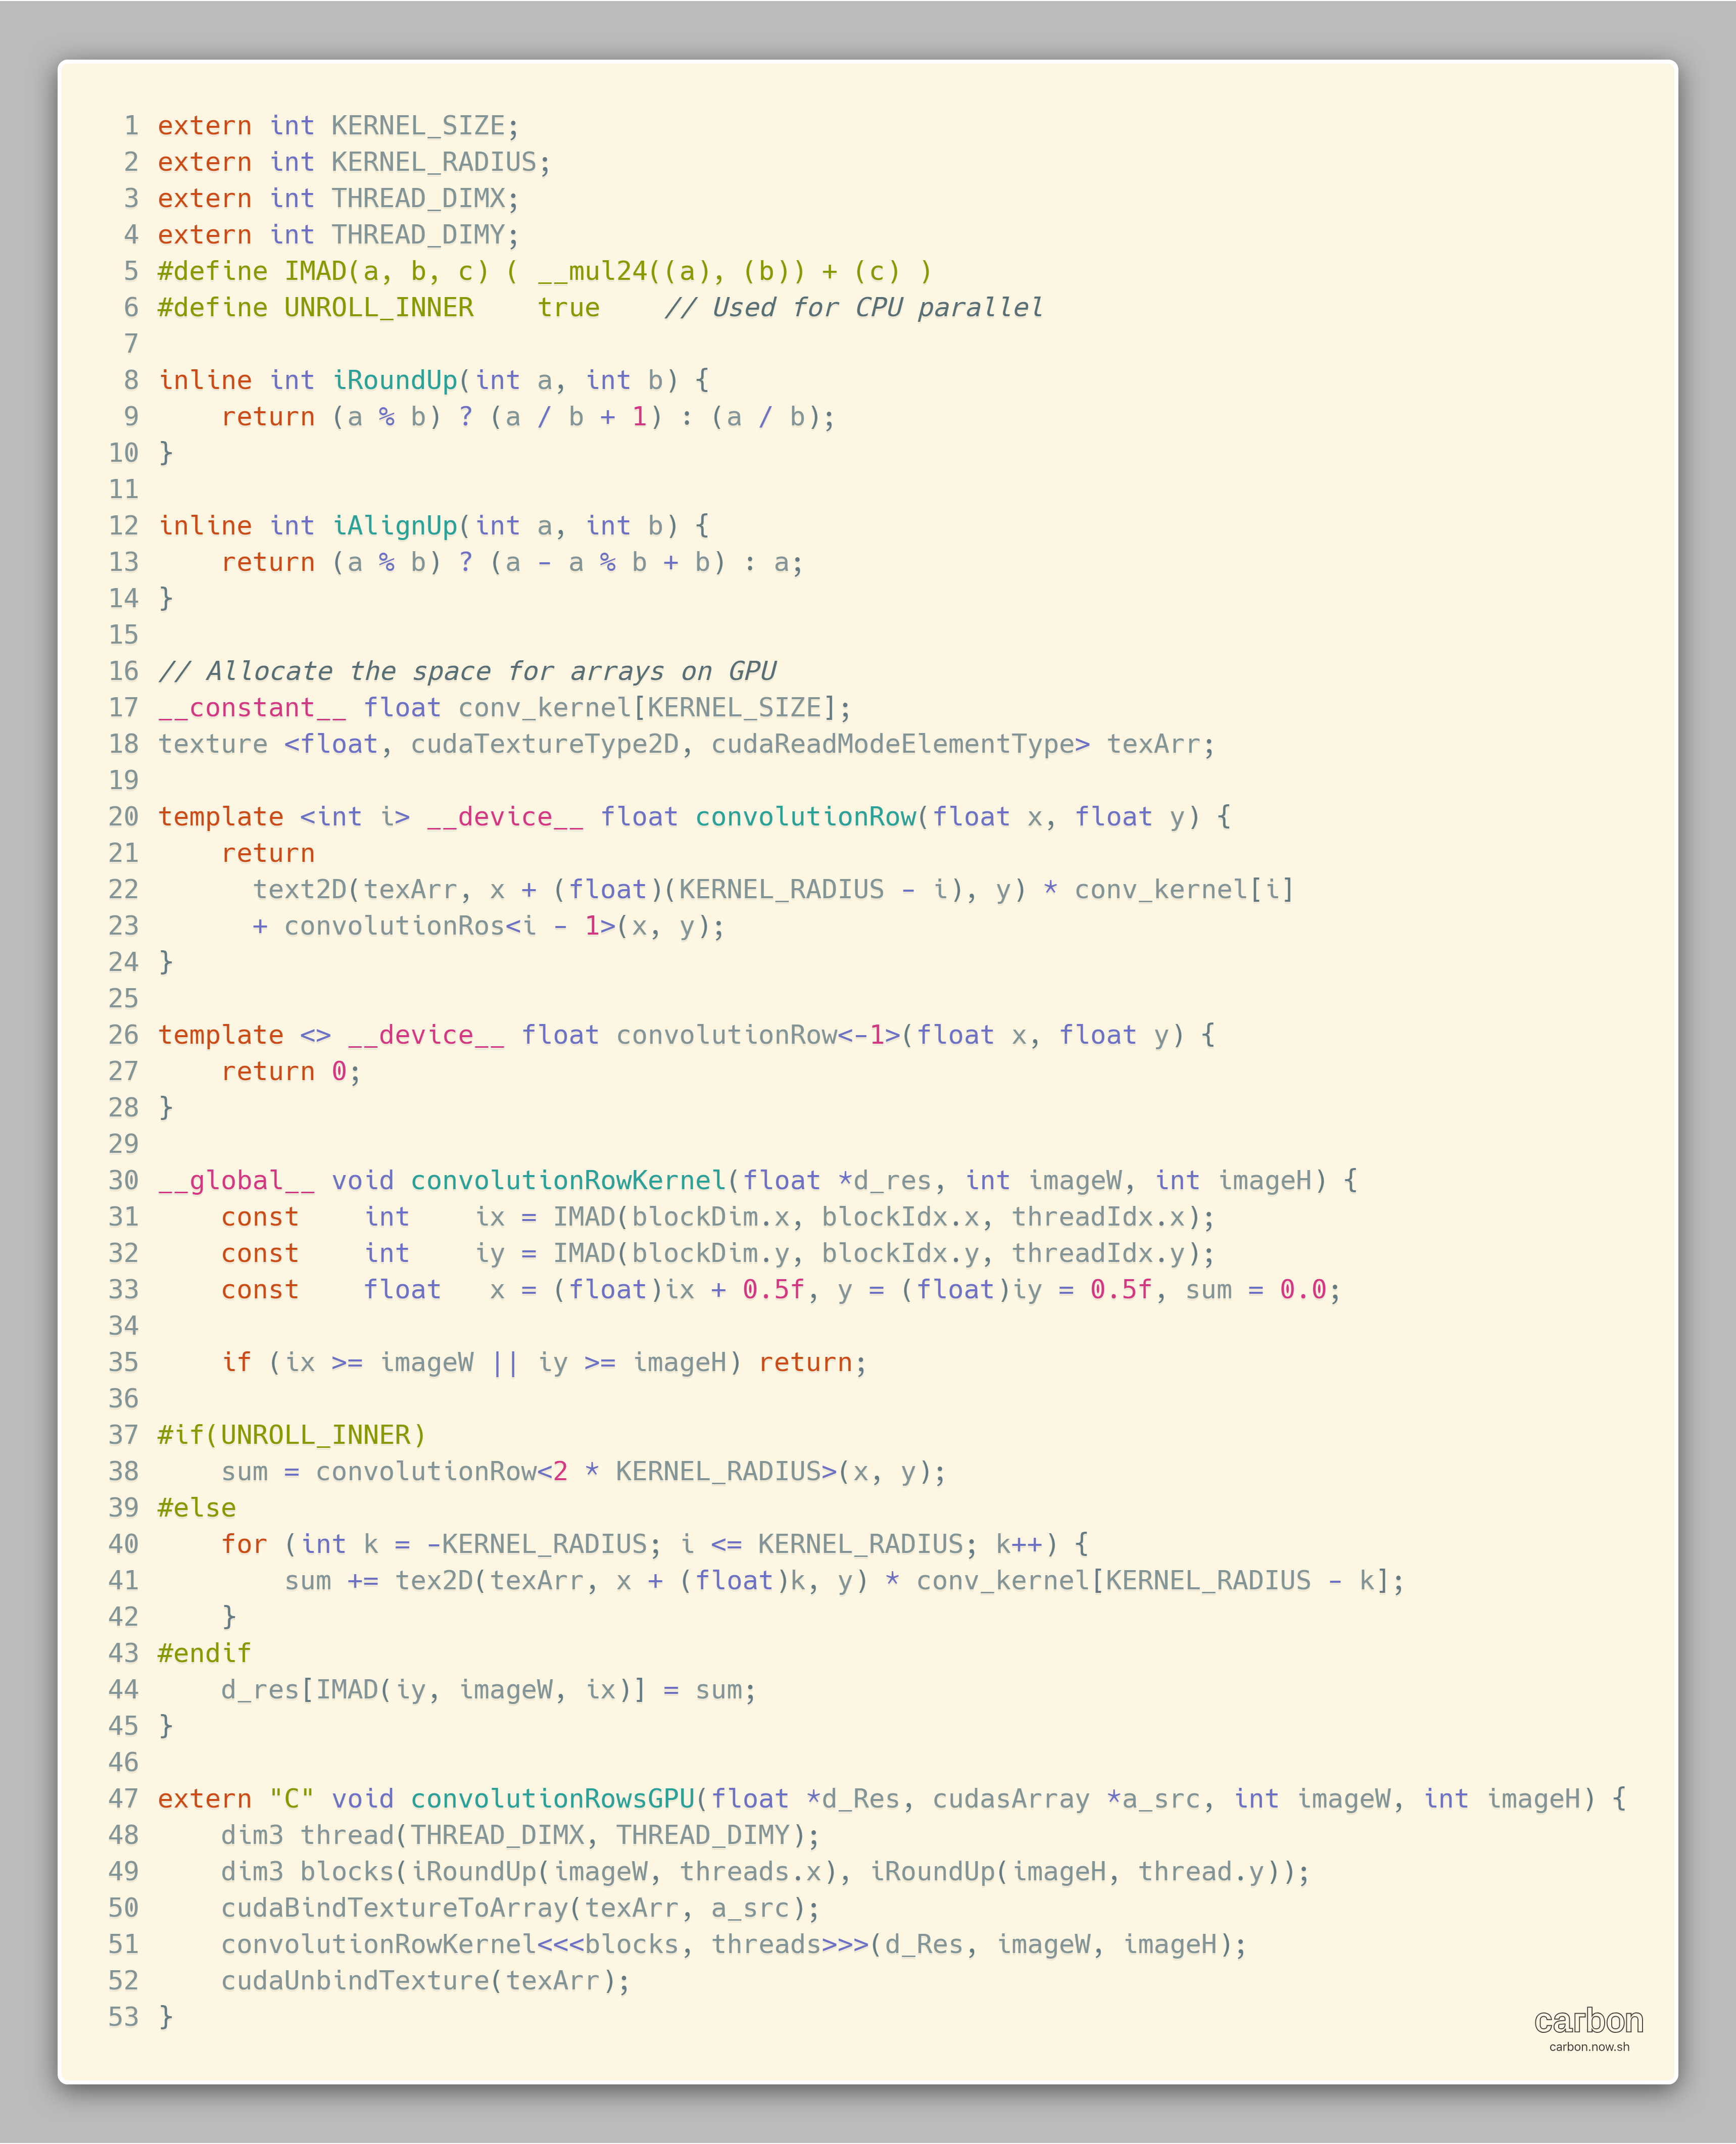
\includegraphics[width=15cm]{figures/TEXSRC.jpg}
	\renewcommand{\thefigure}{\arabic{section}-\arabic{figure} }
	\renewcommand{\figurename}{图}
	\caption{使用纹理内存计算卷积的代码段}
	\addtocounter{figure}{-1}
	\renewcommand{\thefigure}{\arabic{section}-\arabic{figure} }
	\renewcommand{\figurename}{Figure}
	\caption{Part of the code of calculating convolution by texture memory}
	\label{Fig.TexCode}
\end{figure}
\par 需要注意的是,在神经网络中还有一个极为重要的部分便是超参数,在完成对存储系统的研究、优化后,仍将进行对于卷积神经网络中超参数的研究,研究方法与矩阵乘加一节的方式相似。这里挑选了图像通道、卷积核数量、输入批大小等参数进行研究,结果如图 \ref{Fig-CNNMNK}所示。从图中可以直观看出在本实验中的卷积神经网络上,当输入批大小控制在8-16,输入图像的通道数控制在64-512,卷积核数量控制在64-1024个时,前向传播性能的提升尤为明显,进而提升整体性能。需要注意的是由于硬件调度、缓存访问等特性,在该范围内选用2的指数幂能带来较好的性能,然而在实际问题中超参数的选择很大程度上需要为准确性服务,取决于问题本身,所以在实际应用中很难在超参数方面完美地满足硬件地特性。
\begin{figure}
	\centering
	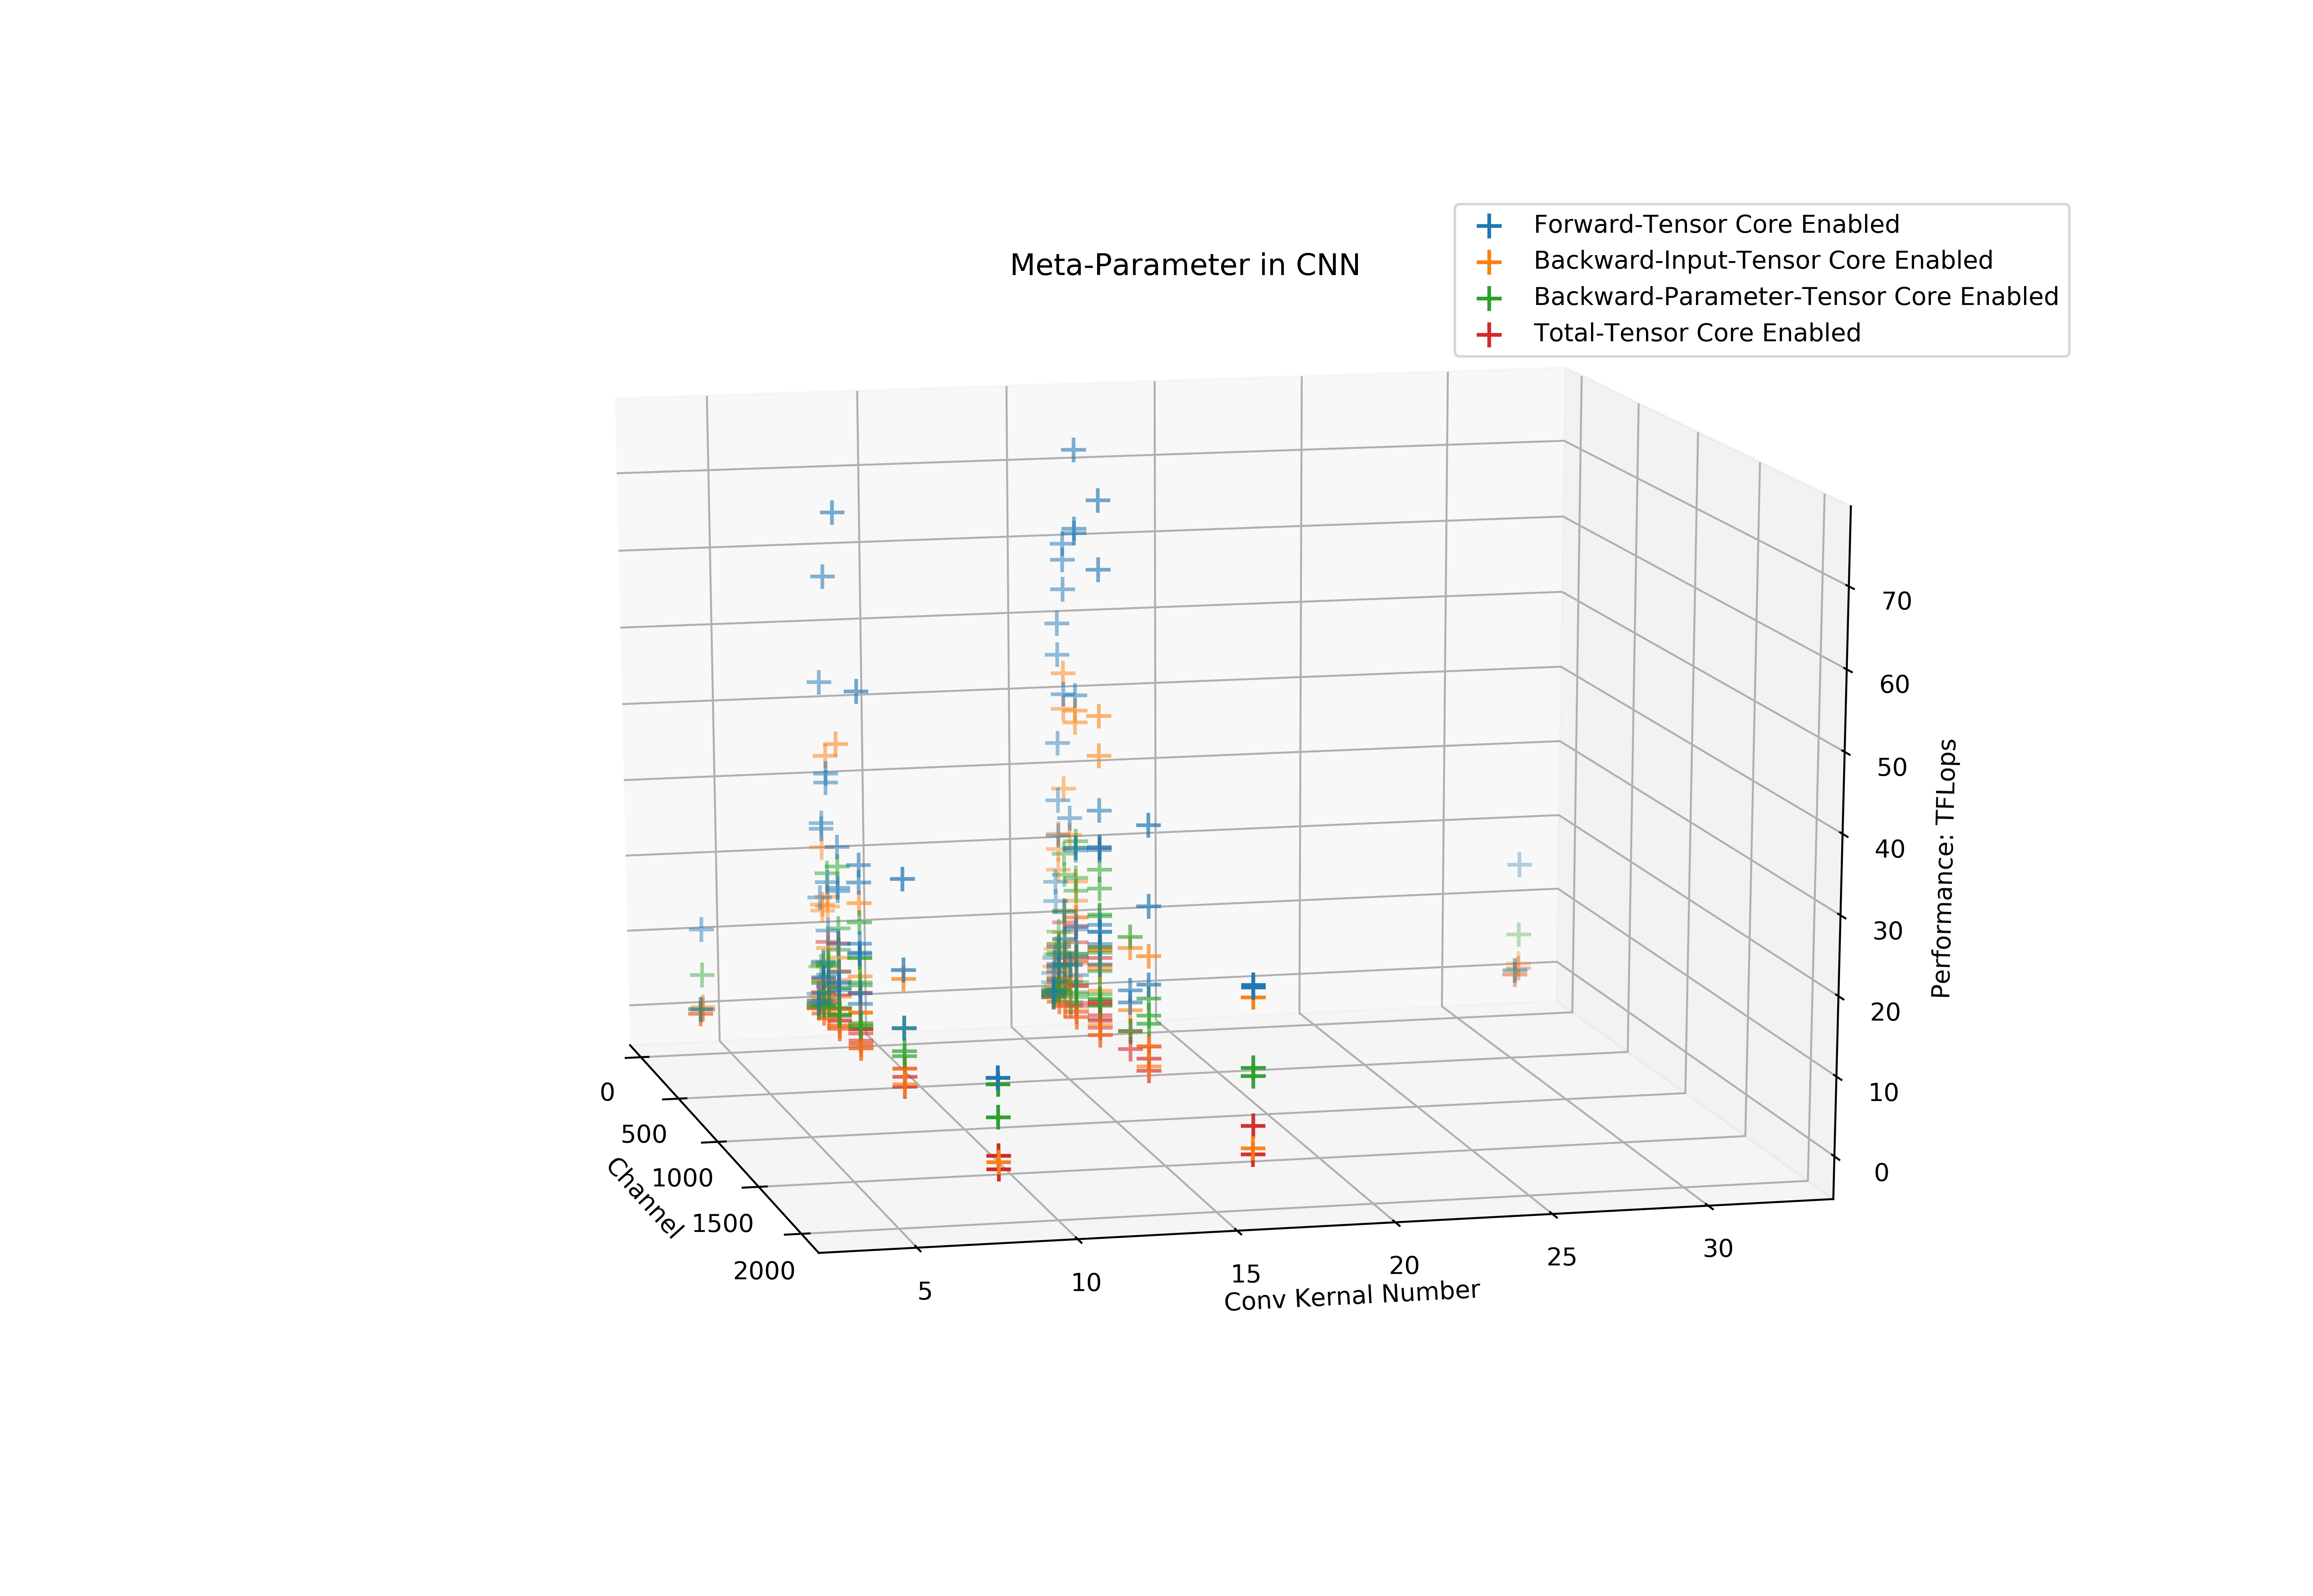
\includegraphics[height=7.2cm]{figures/CNN-CONVN-CH.jpg}\\
	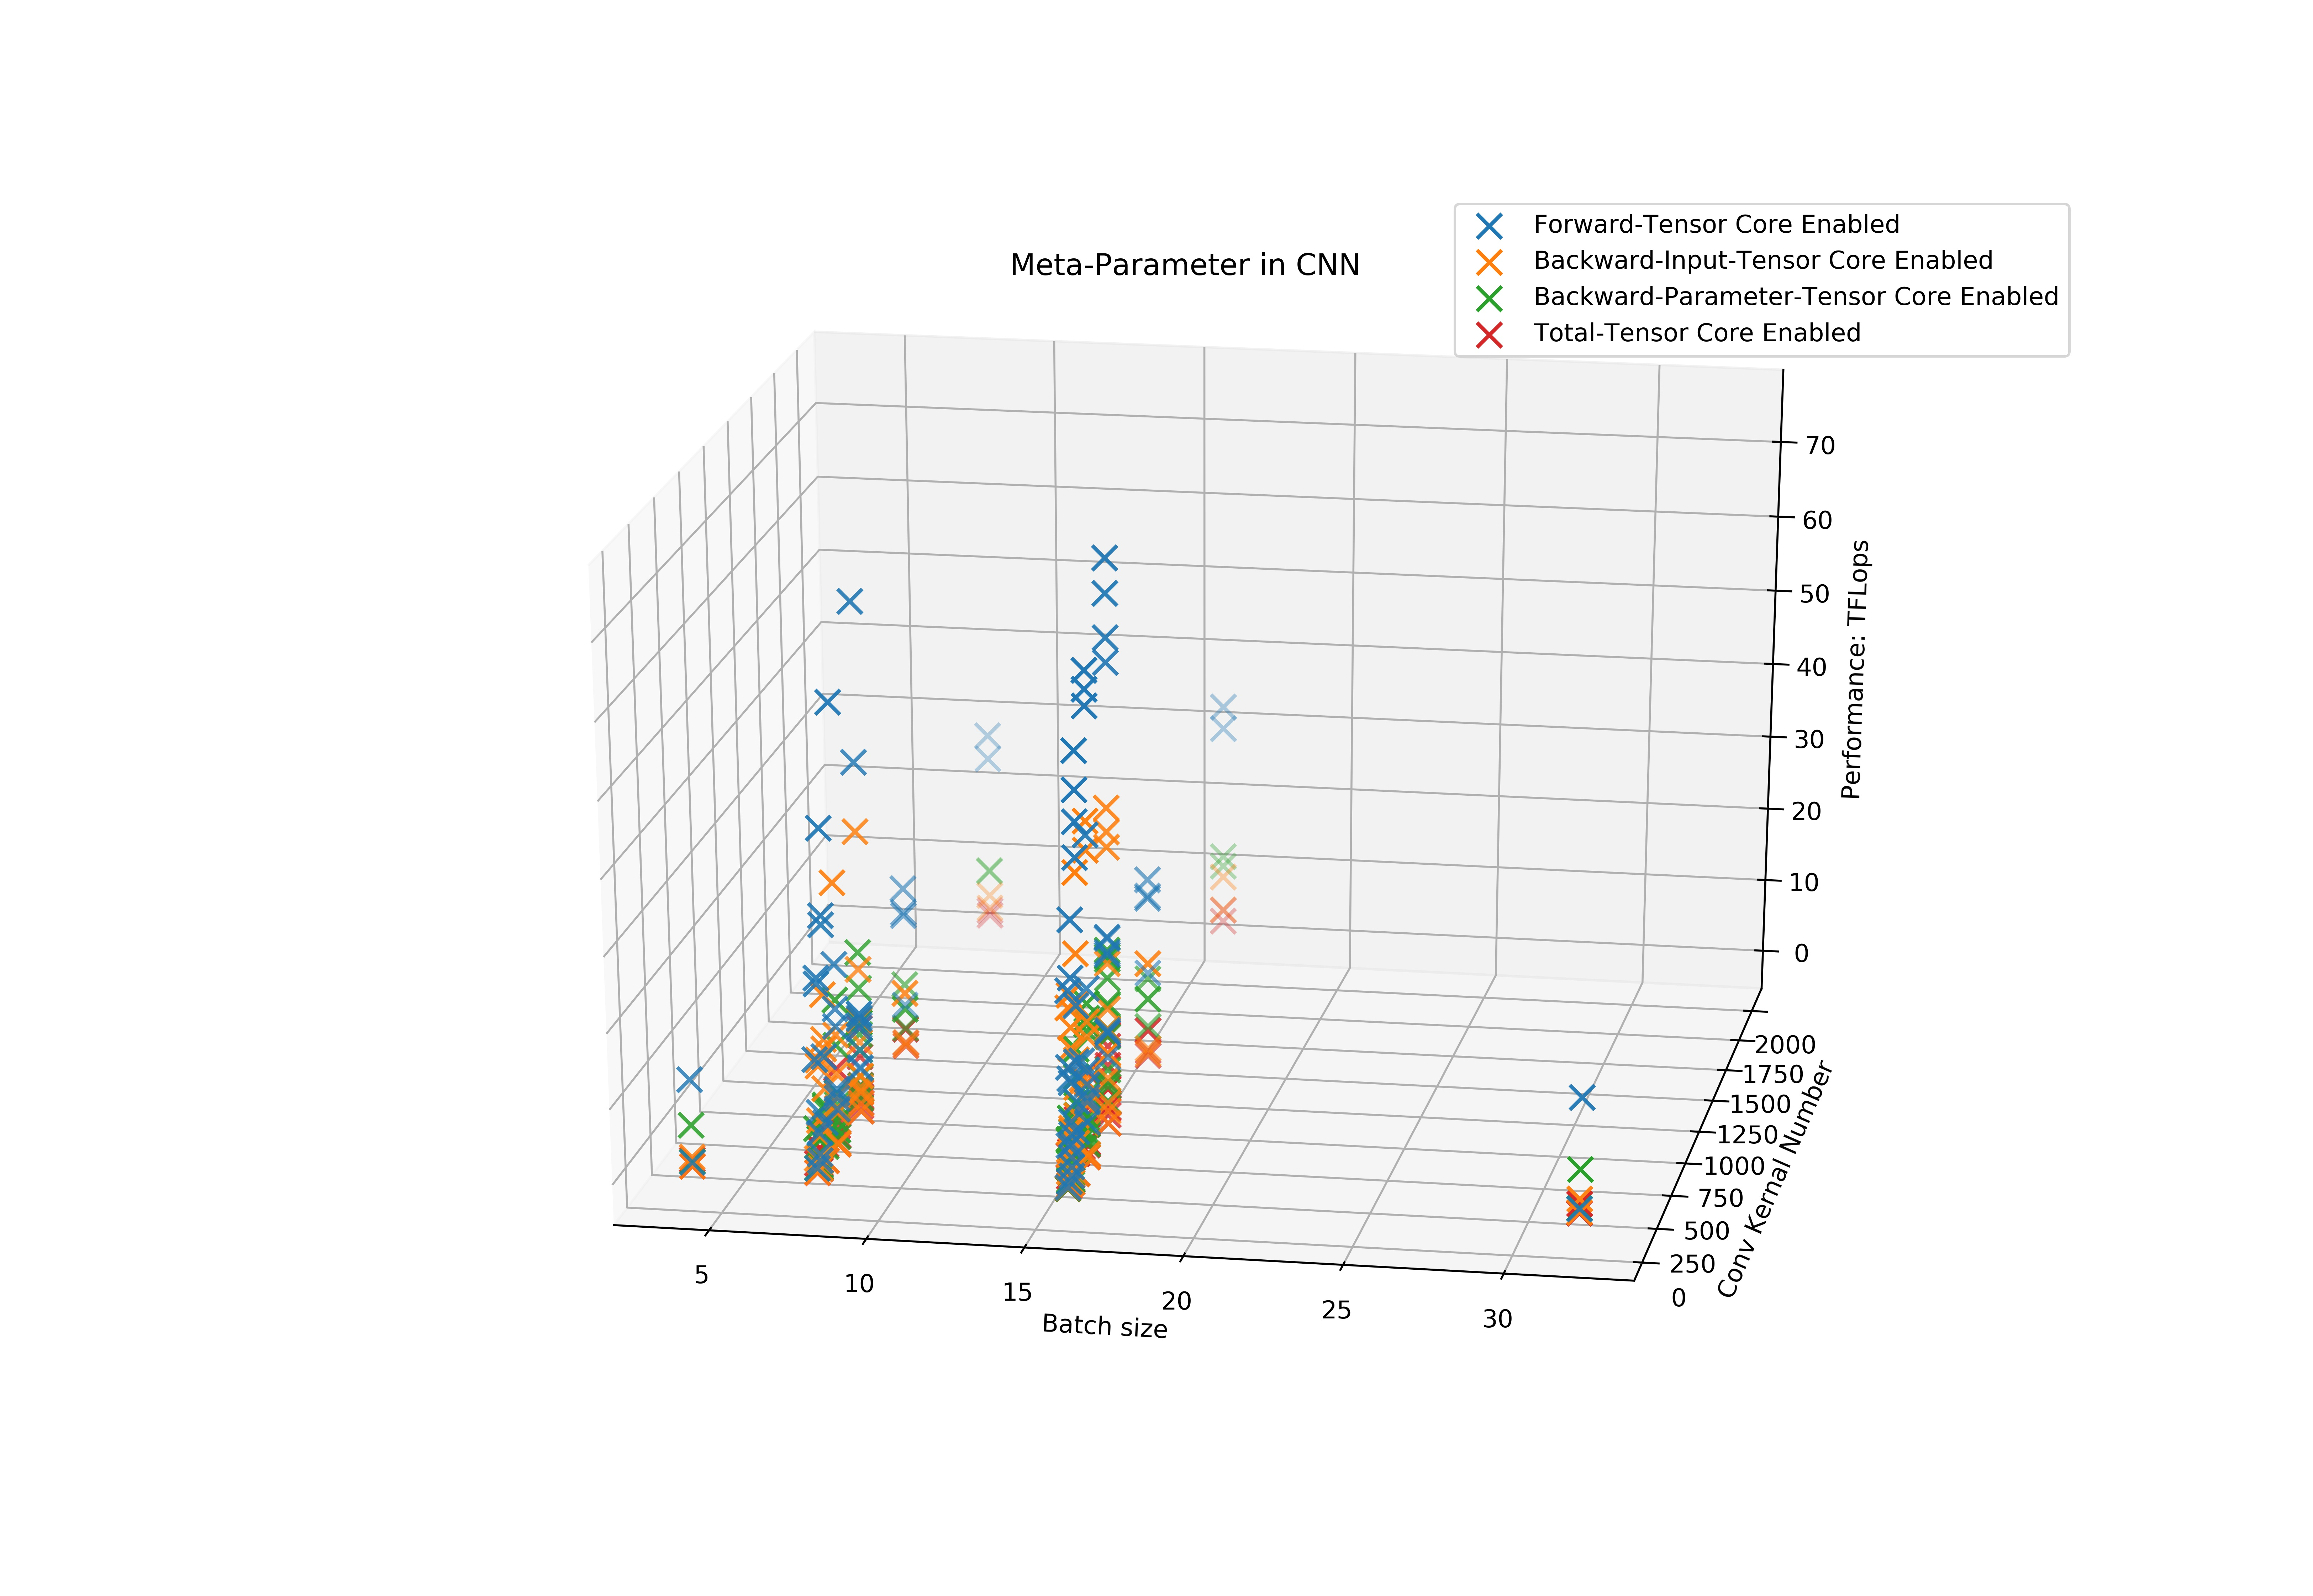
\includegraphics[height=7.2cm]{figures/CNN-CONVN-BS.jpg}\\
	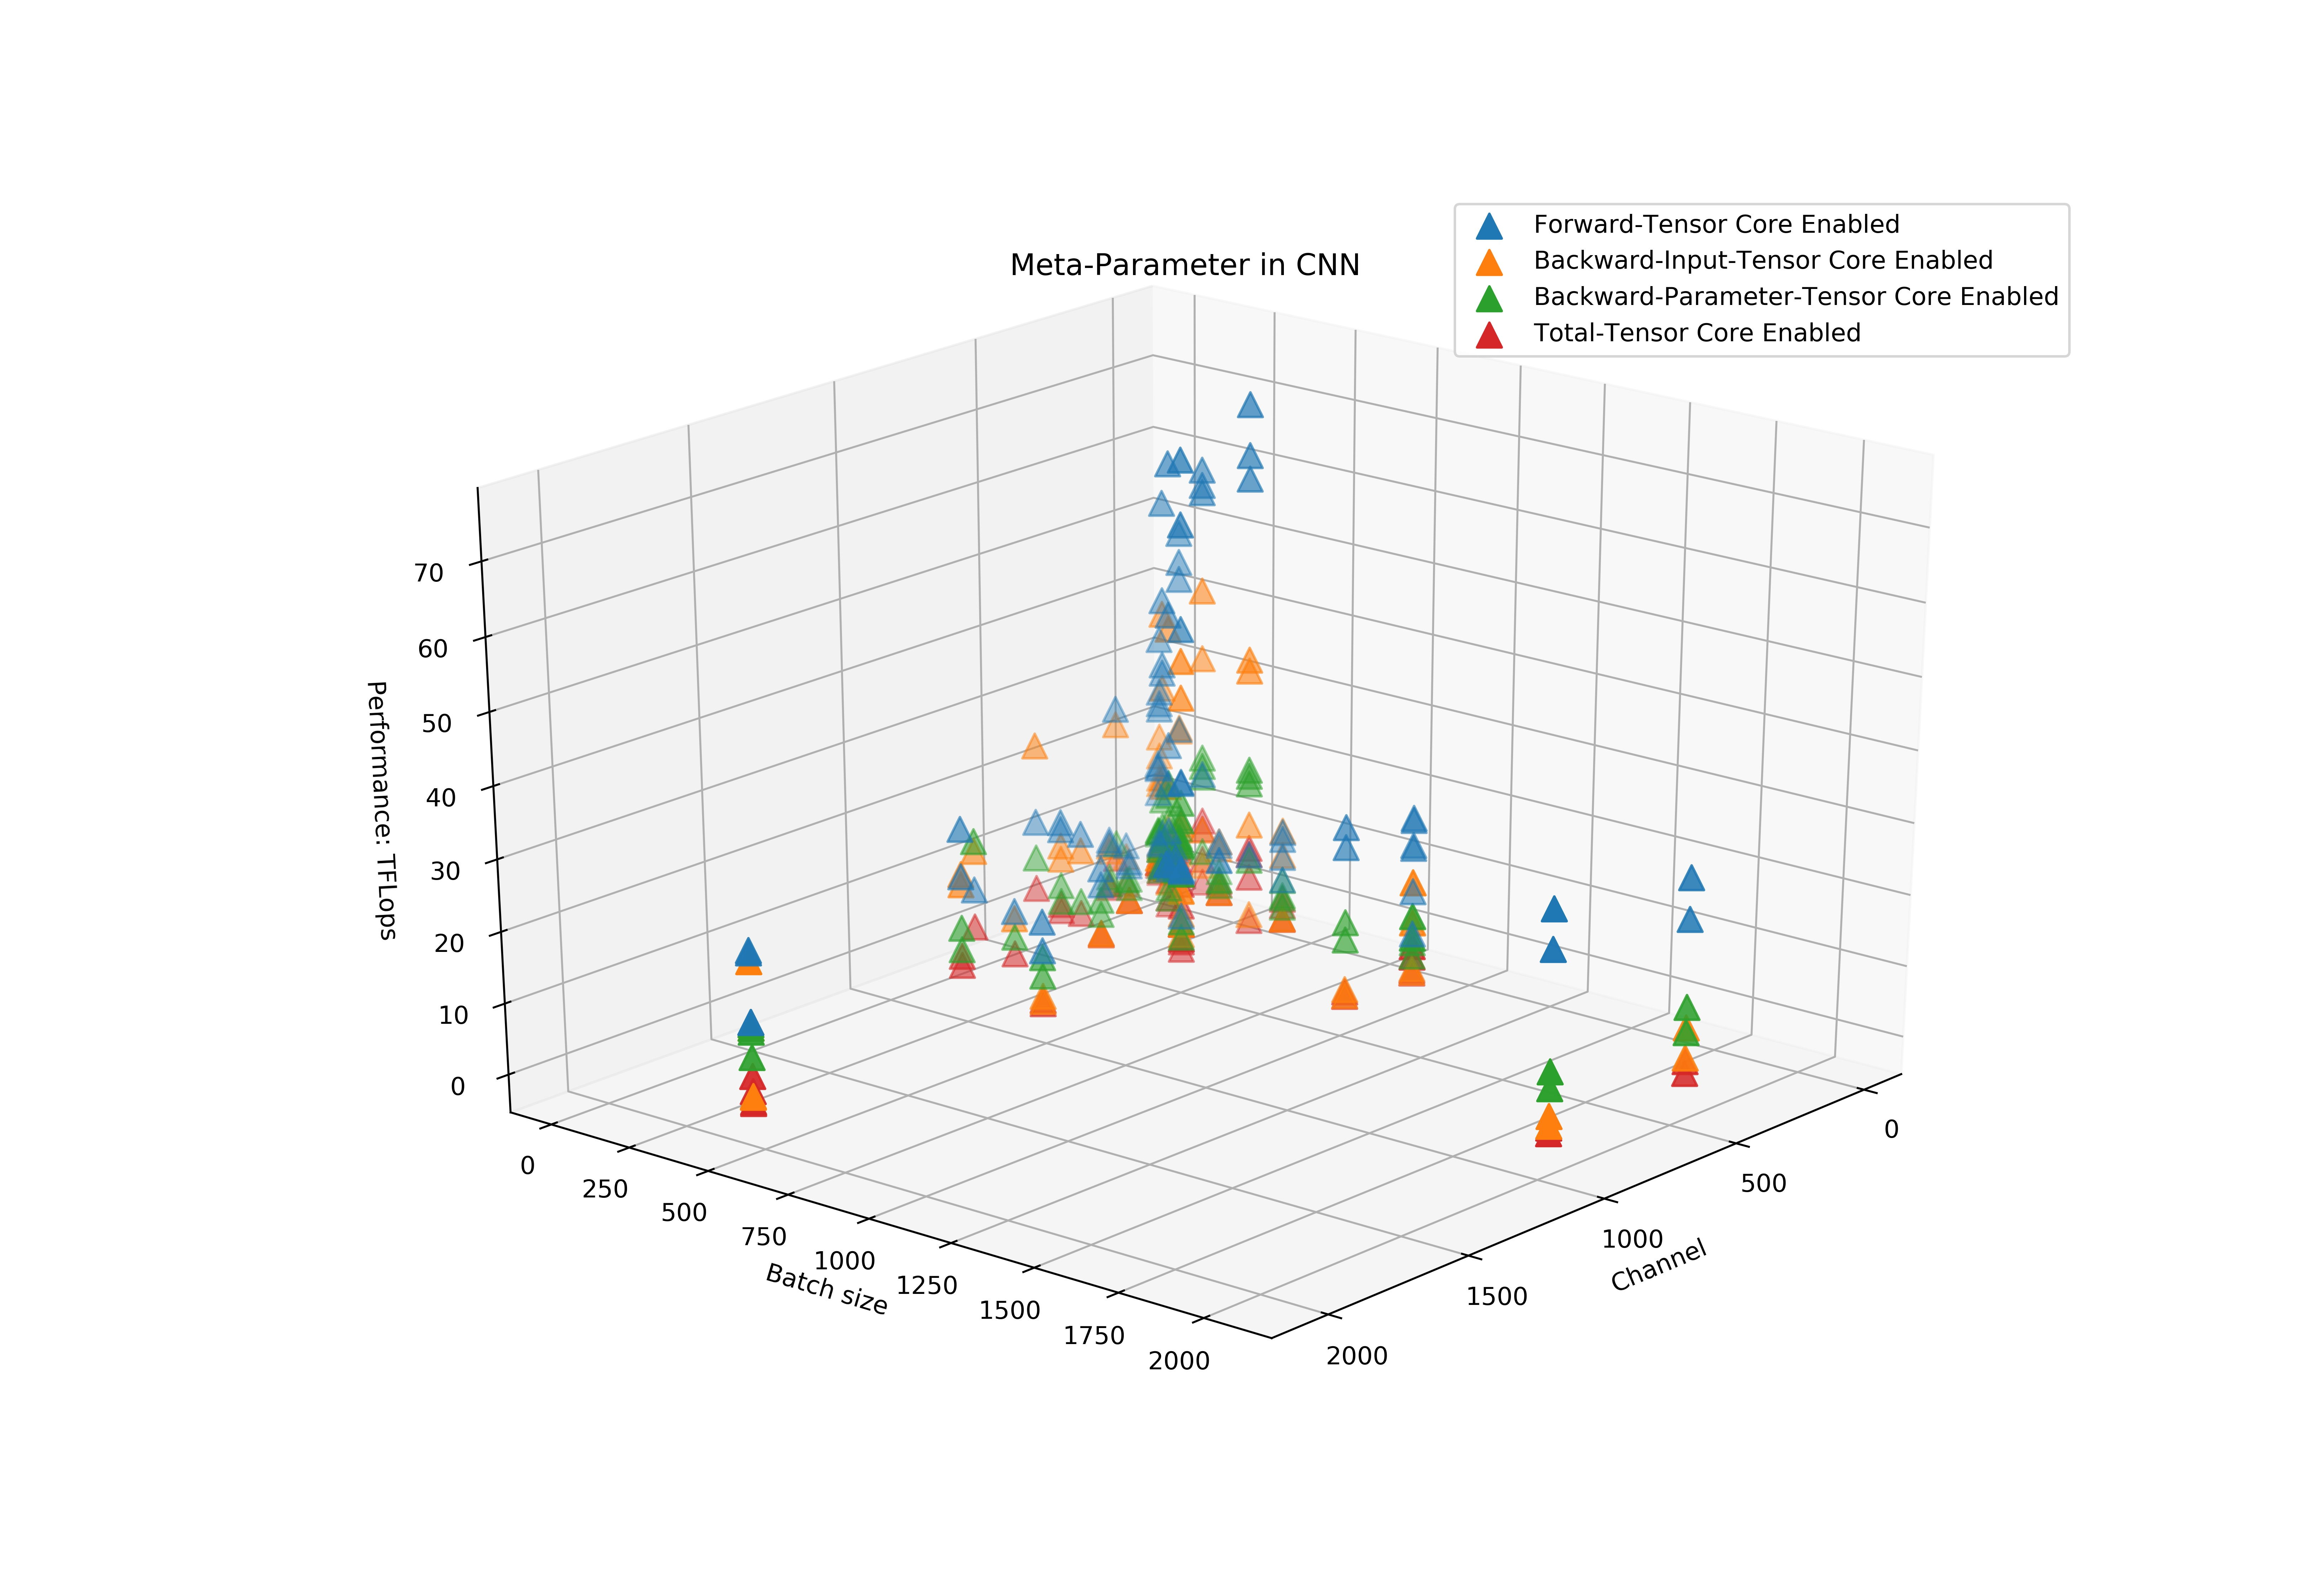
\includegraphics[height=7.2cm]{figures/CNN-CH-BS.jpg}
	\renewcommand{\thefigure}{\arabic{section}-\arabic{figure} }
	\renewcommand{\figurename}{图}
	\caption{卷积神经网络中图像通道、卷积核个数、输入批大小的影响}
	\addtocounter{figure}{-1}
	\renewcommand{\thefigure}{\arabic{section}-\arabic{figure} }
	\renewcommand{\figurename}{Figure}
	\caption{Performance and Channel, amount of Conv kernel, batch size of CNN}
	\label{Fig-CNNMNK}
\end{figure}
\par 由于完整的卷积神经网络结构、运算较复杂,在计算时难免引入许多控制依赖/数据以来,导致无法完美发挥新架构在矩阵运算方面地优势。这种依赖需要通过同步机制解决,然而正如上文所提到的,被组织为线程束地32个线程时同步操作的基本单位,这就意味着在复杂网络中被阻塞的线程数量十分可观,因此可以提出合理的猜想,即在下一代硬件中将会引入更小粒度、更灵活的同步机制,使CUDA的同步机制更加完善。
\subsubsection{并行最小序列优化支持向量机(SMO-SVM)}
\par 前文中出现的评测、研究都是针对深度学习应用的,如网络推理、卷积神经网络等。然而在实际应用中,传统机器学习方法凭借其易于部署、响应时间快、占用资源小、模型本身较小等特点仍然占有很大时长。故本节中选用非常经典的支持向量机算法(Support Vector Machine, SVM),基于SMO并行化。旨在全方位评估实际应用场景中新架构所能带来的性能提升。实验代码和数据集方面选用了并行SVM库thunderSVM,并根据事前得到的实验结果中的结论对源代码进行调整、优化。
\par 支持向量机本质上是求解一个凸优化问题,如公式 (\ref{eqn.SVMRAW})所示,而常见的解决方法为将该优化问题使用拉格朗日函数法转化为对偶问题,如公式 (\ref{eqn.SVMDUAL})所示。在转化后的对偶问题中,需要优化的变量为$ \alpha $,需要注意的是这是一个序列,为SVM的优化,序列最小优化(Sequential Minimal Optimization, SMO)出现了\cite{SMO}。SMO算法的核心思路为通过将原问题分解为一些列小规模凸二次规划问题而获得原问题的解,以$ \alpha $中的两个维度作为迭代时的最小工作集;在每次迭代中,固定除选定的两个维度以外的其他维度,同时采用启发式方式对选定的两个维度进行优化,直至到达停止条件。既然需要将问题分解成子问题,那么其中就有可并行的部分。且优化过程中也涉及矩阵运算,可以利用新硬件中的张量核心进行。
\begin{equation}
\begin{aligned}
&\max_{w, b} \quad \frac{2}{||w||^2} \\
&s.t.\quad y_{i}(w^{T}X_{i}+b) \geq 1
\end{aligned}
\label{eqn.SVMRAW}
\end{equation}
\begin{equation}
\begin{aligned}
&\max_{\alpha} \quad \sum_{i=1}^{N}\alpha_{i} - \frac{1}{2}\sum_{i=1}^{N}\sum_{j=1}^{N}\lbrack \alpha_{i}y_{i}X_{i}^{T}X_{j}y_{j}\alpha_{j} \rbrack \\
&s.t.\quad \sum_{i=1}^{N}\alpha_{i}y_{i}=0, 0 \leq \alpha_{i} \leq C
\end{aligned}
\label{eqn.SVMDUAL}
\end{equation}
\paragraph{实验结果}
\par 实验采用ThunderSVM的支持向量机分类任务和自带的数据集。因任务较为复杂,不方便直接使用TFlops进行性能统计,故直接采用训练时间进行评估。为了延长训练时间,提高时间统计的精确度,本节中的实验简单地扩展了不同规模的数据集,数据集分别包含3000、30000个条目,可被分为3个类。由于支持向量机中仍然存在矩阵运算,故本节仍会开启和关闭张量核心考察性能。需要注意的是,由于样本特征的关系,支持向量机中会涉及较多稀疏矩阵运算,而CUDA有一套专为稀疏矩阵编写的库cuSPARSE,本实验中也会进行评估。表 \ref{table-SMOSVM}列出了四种训练时矩阵的计算方法。选用两种不使用张量核心的GEMM方法的目的在于评估新/老SDK是否会为浮点数值计算的性能带来差距
\begin{table}
	\centering
	\renewcommand{\thetable}{\arabic{section}-\arabic{table} }
	\renewcommand{\tablename}{表}
	\caption{SMO-SVM中使用的矩阵计算方法}
	\addtocounter{table}{-1}
	\renewcommand{\thetable}{\arabic{section}-\arabic{table} }
	\renewcommand{\tablename}{Table}
	\caption{Matrix calculation algorithm in SMO-SVM}
	\begin{tabular}{cc}
		\toprule
		矩阵计算方法 & 描述	\\
		\midrule
		GEMM Legacy & 基于老架构、老SDK的GEMM实现方式\\
		GEMM & 基于新架构、新SDK的不使用张量核心的实现方式\\
		GEMM Tensor Core& 基于新架构、新SDK的使用张量核心的实现方式\\
		cuSPARSE & 基于稀疏矩阵库的实现方式\\
		\bottomrule
	\end{tabular} \label{table-SMOSVM} 
\end{table}
\par 根据图 \ref{Fig-SMOSVMRES}中的实验结果主要有三点发现。一是同样在新架构上,不使用张量核心的两种GEMM方法在数据集较大时,使用新SDK会有5\%-10\%的提升,而数据集较小时提升不明显。可见新SDK在浮点数值计算方面针对新硬件做出了优化,但总体差距不大。二是使用张量核心的GEMM方法能够较明显缩短训练时间,幅度大约在30\%左右。三,也是最重要的结论,在数据集较大时使用稀疏矩阵库cuSPARSE优化后的性能超过了使用张量核心的GEMM的性能。
\begin{figure}
	\centering
	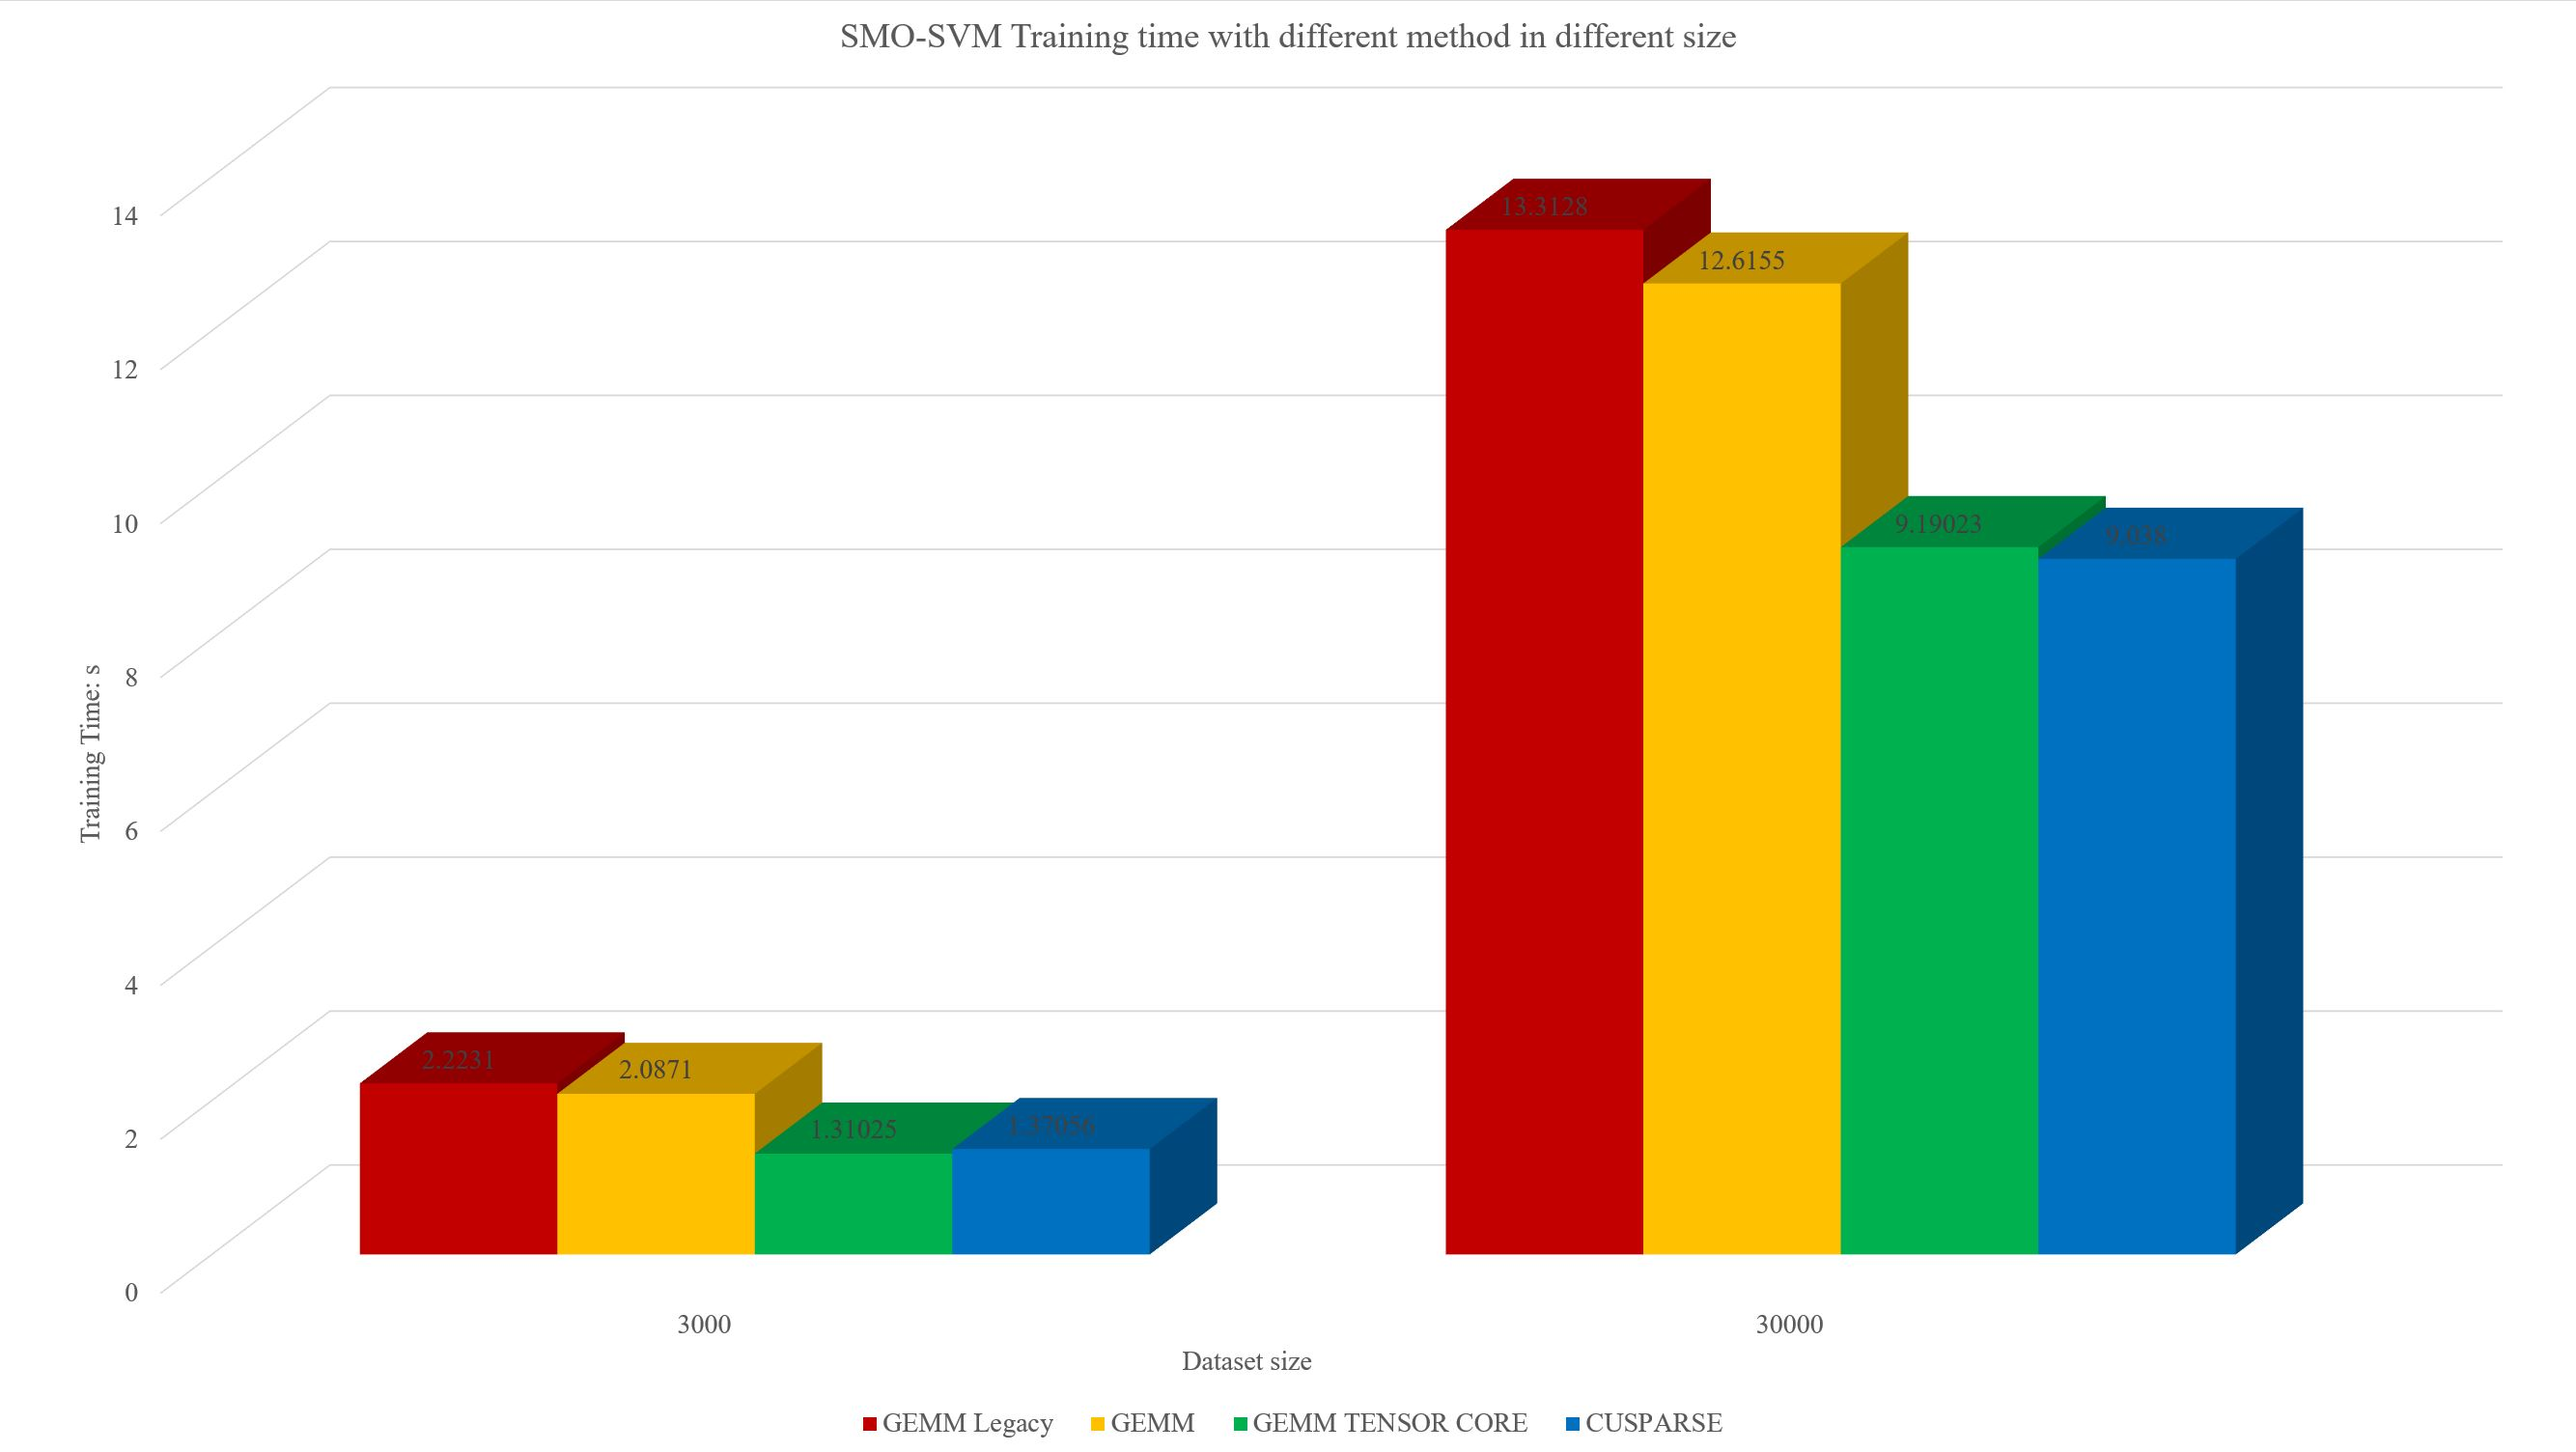
\includegraphics[width=15cm]{figures/SMOSVMRES.jpg}
	\renewcommand{\thefigure}{\arabic{section}-\arabic{figure} }
	\renewcommand{\figurename}{图}
	\caption{SMO-SVM训练时间}
	\addtocounter{figure}{-1}
	\renewcommand{\thefigure}{\arabic{section}-\arabic{figure} }
	\renewcommand{\figurename}{Figure}
	\caption{Training time of SMO-SVM}
	\label{Fig-SMOSVMRES}
\end{figure}
\paragraph{结果分析}
\par 针对实验结果中使用张量核心的GEMM的性能提升幅度,因支持向量机中除去算术运算,还存在诸多逻辑、分支和大量模板库,复杂、多样的计算无法避免,故提升幅度远小于Benchmark中使用张量核心的性能提升幅度。针对稀疏矩阵库cuSPARSE,随着数据集的增大,特征矩阵更为稀疏,采用CSR压缩存储的稀疏矩阵压缩比更高,故cuSPARSE表现较好。而数据集较小时CSR压缩存储的矩阵压缩比较小,节省的运算资源也较少,故性能不如使用张量核心的GEMM。在原始的ThunderSVM库中,采用的是cuSPARSE优化的稀疏矩阵计算方法。本实验中将源代码改为使用张量核心的GEMM方法,并取得了一些性能上的提升。
\par 该结论给出一个启发,在实际编写传统机器学习应用时,涉及到分类、回归等任务时,由于特征抽取中二元特征的存在,其特征矩阵在很多情况下会较为稀疏。在这种情况下不应一味地使用基于张量核心的GEMM,这种情况下将稀疏矩阵转化为CSR矩阵并使用cuSPARSE计算会带来极大的性能提升,尤其是在数据量较大时。而数据量较小、单次矩阵计算粒度较小时,应使用基于张量核心的GEMM。
\subsection{基于TensorFlow框架的应用}
\par 本节选用Tensor Flow作为实验框架,在实验开始进行时,Tensor Flow最新版本为1.12.0,基于CUDA SDK 9.2与cuDNN 7.2进行编译,若要使用CUDA SDK 10.0则需要从源码对框架进行编译。而截至目前,Tensor Flow已经跟新1.13.0版本,该版本支持CUDA SDK 10.0,可以直接通过pip进行安装。在2019年第一季度,NVIDIA发布了CUDA SDK 10.1以及cuDNN 7.5,然而在10.1版本的SDK中主要是对部署时模型大小、特定矩阵运算的精度进行了优化,相关矩阵哭的改动也仅为cuBLASt轻量级库,性能差距不大,故本节仍选用10.0版本的SDK。然而,由于需要针对纹理内存做出优化,故对Tensor Flow底层C++源码进行调整并重新编译是无法避免的。编译方式较为繁琐,已在第二章中介绍,此处不再赘述。
\paragraph{实验结果}
\par 本节使用Tensor Flow框架搭建了基于LeNet-5模型的卷积神经网络,基本结构为数据输入卷积层、进行池化、再卷积、再池化、接入全连接采用Softmax进行分类。数据集采用cifar-10,包含50000张$ 32 \times 32 $像素的RGB图像,可被分为十个不同的类。相对于网络精确度,本文更关心网络的训练、推理速度,故这里采用这种结构简单但是完整,能全方位体现Tensor Flow使用GPU加速性能的网络结构,该网络结构能在cifar-10数据集上达到69\%的预测准确率。在考察基本性能后,将根据上文实验得到的结论对网络Python级别代码、Tensor Flow的C++级别源码进行更改,力求再保证精度的情况下达到更快的训练、推理速度。
\par 根据上文的实验结果,对于深度学习模型,主要可改进如下方面:再训练部分使用张量核心加速矩阵乘加运算,使用较低的精度换更快的速度,在使用张量核心的情况下优化超参数使其适合张量核心进行运算,在输入图像尺寸较小时使用直接方法并借助纹理内存计算卷积以及在推理部分使用TensorRT对网络推理进行加速。由于最新版本的Tensor Flow默认开启张量核心,故本节实验不再对是否开启张量核心进行评估。具体评估条目如表 \ref{table-TFList}所示。
\begin{table}
	\centering
	\renewcommand{\thetable}{\arabic{section}-\arabic{table} }
	\renewcommand{\tablename}{表}
	\caption{基于Tensor Flow框架的CNN的改进}
	\addtocounter{table}{-1}
	\renewcommand{\thetable}{\arabic{section}-\arabic{table} }
	\renewcommand{\tablename}{Table}
	\caption{Improvment in CNN based on Tensor Flow}
	\begin{tabular}{cc}
		\toprule
		项目 & 说明\\
		\midrule
		低精度代替高精度 & 训练中使用FP16、INT8代替FP32\\
		优化超参数 & 网络中超参数包括批大小、卷积核尺寸等\\
		改进卷积方式 & 在Tensor Flow源码中(eigen\_spatial\_convolutions.h)更改卷积计算方式\\
		TensorRT加速推理 & 在网络推理阶段使用Jetson TX2与TensorRT加速推理\\
		\bottomrule
	\end{tabular} \label{table-TFList} 
\end{table}
\par 该实验涉及各方面的运算,很难使用TFlops等指标进行评估,故直接采用网络训练、推理时间,使用时间也比较直观。因变量过多,这里采用控制变量的方法,每次实验只更改一种项目,并计算与基准时间的差别。下表为实验结果,其中被标记为蓝色的为原始代码中的数值,作为基准;被标记为红色的会带来极大的网络准确率下降;被标记为黄色的会带来较小的准确率下降,所有数据均为相对于原训练时间的倍数,故越小代表训练时间越短。实验结果如表 \ref{table-TFRES}所示,表中蓝色条目为原始网络的参数,橙色条目为使网络分类准确率小幅下降的调节参数,而红色条目则为使网络分类准确率大幅下降的调节参数。
\begin{table}
	\centering
	\renewcommand{\thetable}{\arabic{section}-\arabic{table} }
	\renewcommand{\tablename}{表}
	\caption{基于Tensor Flow框架的CNN的优化结果}
	\addtocounter{table}{-1}
	\renewcommand{\thetable}{\arabic{section}-\arabic{table} }
	\renewcommand{\tablename}{Table}
	\caption{Optimization result in CNN based on Tensor Flow}
	\begin{tabular}{cccccccc}
		\toprule
		基准时间 &  超参数更改 &更改方式 &时间倍率 & 计算精度 &时间倍率 & 卷积方式 &时间倍率 	\\
		\midrule
		54.016(s) & 批大小 & 16 & $ \times17.07 $ & \color[rgb]{0.3,0.4,1.0}{FP32} & \color[rgb]{0.3,0.4,1.0}{$ \times 1 $ } & \color[rgb]{0.3,0.4,1.0}{原始(GEMM)} &\color[rgb]{0.3,0.4,1.0}{$ \times 1 $} \\
		 & & 32 & $ \times 5.21 $ & \color[rgb]{0.9,0.7,0.01}{FP16} & \color[rgb]{0.9,0.7,0.01}{$ \times 0.86 $} & 纹理$ ** $ & $ \times 0.94 $\\
		 & & 64 & $ \times 2.10 $ & \color[rgb]{0.9,0.7,0.01}{INT8} & \color[rgb]{0.9,0.7,0.01}{$ \times 0.82 $} & FFT & $ \times 1.11 $\\
		 & & \color[rgb]{0.3,0.4,1.0}{128} & \color[rgb]{0.3,0.4,1.0}{$ \times 1 $}& & & & \\
		 & & 256 & $ \times 0.51 $ & & & & \\
		 & & 512 & $ \times 0.31 $ & & & & \\
		 & & \color[rgb]{0.9,0.7,0.01}{1024} & \color[rgb]{0.9,0.7,0.01}{$ \times 0.21 $}& & & & \\
		 & 卷积核 & \color[rgb]{0.3,0.4,1.0}{$ 5\times 5 $} & \color[rgb]{0.3,0.4,1.0}{$ \times 1 $} & & & & \\
		 & & \color{red}{$ 8\times 8 * $} & \color{red}{$ \times 0.97 $} & & & & \\
		\bottomrule
	\end{tabular} \label{table-TFRES} 
$ * $卷积核尺寸修改会牵连到整个网络的连接结构\\
$ ** $直接方式计算卷积辅以纹理内存在kernel\_op.h与eigen\_spatial\_convolution.h中修改
\end{table}
\par 以上是训练部分的结果,在网络推理部分,使用TensorRT优化前的模型在Jetson TX2上的推理速度是每张图片由输入至输出分类信息花费59毫秒,而优化后的模型推理时间缩减为32毫秒。
\paragraph{结果分析}
\par 根据实验结果可以得出如下结论:
\begin{itemize}
	\item 从理论上来说,使用GPU进行大规模计算时应尽可能增加一次处理同时处理的数据量,在本实验中即为批大小。然而过大的批大小会减少迭代次数,对网络准确率造成一定影响。故实际应用中应权衡批大小与准确率,在保证精度的情况下尽可能加大批大小。
	\item 关于卷积核大小的调整,在卷积神经网络相关论文中有详细的讨论,其调整需要基于输入图像特征、任务特征等算法、软件层面的因素,这里不做过多讨论;仅根据结果分析,调整卷积核大小后性能提升较小,这也与上文中实验结果吻合:卷积核大小对于同一图像尺寸在卷积计算速度上影响不大。然而因为网络结构的更爱、特征提取的变化,网络准确率大幅下降,大于10\%,故不推荐对确定好的模型中的卷积核大小进行更改。
	\item 关于网络精度,使用更低的精度能为性能带来显著提升,但是会稍稍降低网络准确率,故实际应用中应柑橘需求权衡是否要“用精度换速度”。
	\item 关于卷积的计算方式,由于本实验中数据集图像大小仅为$ 32\times 32\times 3 $,根据对于卷积性能的实验结果,在小图片中使用纹理内存的直接方法计算卷积能显著提升性能。然而在输入图像较大时这一方法渐渐丧失优势,且随着CUDA SDK的更新,纹理内存的使用逐渐被共享内存的应用取代。尤其是采用这种方式涉及对Tensor Flow底层源码的更改以及再编译,在实际应用中不推荐进行这样的更改。
	\item 在网络推理部分,使用TensorRT优化后推理速度提升显著,这也是因为本实验中网络结构较为简单,计算流合成后效率较高。原先59毫秒的推理延迟意味着在实时视频处理中的帧数不满20帧,这无疑无法满足当前需求;而优化后的推理延迟降为32毫秒,在实时视频处理中帧数达到20帧以上,基本能够满足需求。故在网络的实际部署阶段,条件允许的情况下应尽量使用TensorRT进行优化。其主要障碍是目前只有有限的硬件能使用TensorRT优化并运行模型。
\end{itemize}